%%%%%%%%%%%%%%%%%%%%%%%%%%%%%%%%%%%%%%%%%%%%%%
%
%       Exact Sampling for Classical and Quantum Many-Body Systems
%
%       Based on the EPFL EDOC Template
%       2024
%
%%%%%%%%%%%%%%%%%%%%%%%%%%%%%%%%%%%%%%%%%%%%%%

% LTeX: enabled=false

\documentclass[a4paper,11pt]{book}

\usepackage{iftex}
\ifxetex
\else
    \pdfoutput=1
    \usepackage[T1]{fontenc}
    \usepackage[utf8]{inputenc}
\fi

% Load setspace before hyperref https://github.com/schlcht/microtype/issues/11
\usepackage{setspace} % increase interline spacing slightly
\setstretch{1.1}

\usepackage{doi}
\usepackage[autostyle]{csquotes}
\usepackage[
    backend=biber,
    style=numeric-comp,
    date=year,
    giveninits=true,
    sorting=none,
    url=false,
    doi=true,
    eprint=true,
]{biblatex}
\addbibresource{tail/bibliography.bib}

\usepackage[french,english]{babel}

%%%%%%%%%%%%%%%%%%%%%%%%%%%%%%%%%%%%%%%%%%%%%%%
%% EDOC THESIS TEMPLATE: Variant 1.0 -> Latin modern, large text width & height
%%%%%%%%%%%%%%%%%%%%%%%%%%%%%%%%%%%%%%%%%%%%%%%
% \usepackage{lmodern} % use this to fix blurry typewriter text font
% \usepackage[a4paper,top=22mm,bottom=28mm,inner=35mm,outer=25mm]{geometry}
%%%%%%%%%%%%%%%%%%%%%%%%%%%%%%%%%%%%%%%%%%%%%%%

%%%%%%%%%%%%%%%%%%%%%%%%%%%%%%%%%%%%%%%%%%%%%%
% EDOC THESIS TEMPLATE: Variant 2.0 -> Utopia, Gabarrit A (lighter pages)
%%%%%%%%%%%%%%%%%%%%%%%%%%%%%%%%%%%%%%%%%%%%%%
\ifxetex
    \usepackage{mathtools}
    \usepackage{unicode-math}
    \setmathfont{Erewhon Math}
    \usepackage{erewhon}
\else
    \usepackage{fourier} % Utopia font-typesetting including mathematical formula compatible with newer TeX-Distributions (> 2010)
    % \usepackage{utopia} % on older systems -> use this package instead of fourier in combination with mathdesign for better looking results
    % \usepackage[adobe-utopia]{mathdesign}
\fi
\setlength{\textwidth}{146.8mm} % = 210mm - 37mm - 26.2mm
\setlength{\oddsidemargin}{11.6mm} % 37mm - 1in (from hoffset)
\setlength{\evensidemargin}{0.8mm} % = 26.2mm - 1in (from hoffset)
\setlength{\topmargin}{-2.2mm} % = 0mm - 1in + 23.2mm
\setlength{\textheight}{221.9mm} % = 297mm - 29.5mm - 31.6mm - 14mm (12 to accomodate footline with pagenumber)
\setlength{\headheight}{14mm}
%%%%%%%%%%%%%%%%%%%%%%%%%%%%%%%%%%%%%%%%%%%%%%

\makeatletter
\setlength{\@fptop}{0pt} % for aligning all floating figures/tables etc... to the top margin
\makeatother

\usepackage{graphicx}
\usepackage{xcolor}
\graphicspath{{images/}}

\usepackage{booktabs}
\usepackage{lipsum}
\ifxetex
\else
    \usepackage{microtype}
\fi
\usepackage{subfig}
\usepackage{url}

\usepackage{fancyhdr}
\renewcommand{\sectionmark}[1]{\markright{\thesection\ #1}}
\pagestyle{fancy}
    \fancyhf{}
    \renewcommand{\headrulewidth}{0.4pt}
    \renewcommand{\footrulewidth}{0pt}
    \fancyhead[OR]{\bfseries \nouppercase{\rightmark}}
    \fancyhead[EL]{\bfseries \nouppercase{\leftmark}}
    \fancyfoot[EL,OR]{\thepage}
\fancypagestyle{plain}{
    \fancyhf{}
    \renewcommand{\headrulewidth}{0pt}
    \renewcommand{\footrulewidth}{0pt}
    \fancyfoot[EL,OR]{\thepage}
}
\fancypagestyle{addpagenumbersforpdfimports}{
    \fancyhead{}
    \renewcommand{\headrulewidth}{0pt}
    \fancyfoot{}
    \fancyfoot[RO,LE]{\thepage}
}

\usepackage{listings}
\lstset{
    language=[LaTeX]Tex,
    tabsize=4,
    basicstyle=\scriptsize\ttfamily,
    showstringspaces=false,
    numbers=left,
    numberstyle=\tiny,
    numbersep=10pt,
    breaklines=true,
    breakautoindent=true,
    breakindent=10pt,
}

\usepackage{hyperref}
\hypersetup{
    pdfborder={0 0 0},
    colorlinks=true,
    linkcolor=black,
    citecolor=black,
    urlcolor=black,
}
\urlstyle{same}
\ifxetex
\else
    \ifpdf
        \usepackage[final]{pdfpages}
    \else
        \usepackage{breakurl}
        \usepackage{calc}
        \usepackage[nlwarning=false]{hypdvips}
        \usepackage{backref}
        \renewcommand*{\bacref}[1]{}
    \fi
\fi
\usepackage{bookmark}

\makeatletter
\renewcommand\@pnumwidth{20pt}
\makeatother

\makeatletter
\def\cleardoublepage{
    \clearpage
    \if@twoside
        \ifodd
            \c@page
        \else
            \hbox{}
            \thispagestyle{empty}
            \newpage
            \if@twocolumn
                \hbox{}
                \newpage
            \fi
        \fi
    \fi
}
\makeatother
\clearpage{\pagestyle{plain}\cleardoublepage}

%%%%% CHAPTER HEADER %%%%
\usepackage{color}
\usepackage{tikz}
\usepackage[explicit]{titlesec}
\newcommand*\chapterlabel{}
% \renewcommand{\thechapter}{\Roman{chapter}}
\titleformat{\chapter}[display] % type (section, chapter, etc...) to vary, shape (eg display-type)
    {\normalfont\bfseries\Huge} % format of the chapter
    {\gdef\chapterlabel{\thechapter\ }} % the label
    {0pt} % separation between label and chapter-title
    {
    \ifxetex
        \setlength{\unitlength}{9mm}
    \else
        \setlength{\unitlength}{0mm}
    \fi
    \begin{tikzpicture}[remember picture,overlay]
        \node[yshift=-8cm] at (current page.north west)
        {\begin{tikzpicture}[remember picture,overlay]
            \draw[fill=black] (0,0) rectangle(35.5mm,15mm);
            \node[anchor=north east,yshift=-7.2cm-\unitlength,xshift=34mm,minimum height=30mm,inner sep=0mm] at (current page.north west)
                {\parbox[top][30mm][t]{15mm}{\raggedleft \rule{0cm}{0.6cm}\color{white}\chapterlabel}}; % the empty rule is just to get better base-line alignment
            \node[anchor=north west,yshift=-7.2cm-\unitlength,xshift=37mm,text width=\textwidth,minimum height=30mm,inner sep=0mm] at (current page.north west)
                {\parbox[top][30mm][t]{\textwidth}{\rule{0cm}{0.6cm}\color{black}#1}};
        \end{tikzpicture}};
    \end{tikzpicture}
    \gdef\chapterlabel{}
    } % code before the title body
\titlespacing*{name=\chapter,numberless}{-3.7cm}{83.2pt-\parskip}{-3.2pt+\parskip}
\titlespacing*{\chapter}{-3.7cm}{50pt-\parskip-\parskip}{30pt+\parskip+\parskip}

\titlespacing*{\section}{0pt}{13.2pt}{1em-\parskip} % 13.2pt is line spacing for a text with 11pt font size
\titlespacing*{\subsection}{0pt}{13.2pt}{1em-\parskip}
\titlespacing*{\subsubsection}{0pt}{13.2pt}{1em-\parskip}
\titlespacing*{\paragraph}{0pt}{13.2pt}{1em-\parskip}

\newcounter{myparts}
\newcommand*\partlabel{}
\titleformat{\part}[display] % type (section, chapter, etc...) to vary, shape (eg display-type)
    {\normalfont\bfseries\Huge} % format of the part
    {\gdef\partlabel{\thepart\ }} % the label
    {0pt} % separation between label and part-title
    {
    \ifxetex
        \setlength{\unitlength}{20mm}
    \else
        \ifpdf
            \setlength{\unitlength}{20mm}
        \else
            \setlength{\unitlength}{0mm}
        \fi
    \fi
    \addtocounter{myparts}{1}
    \begin{tikzpicture}[remember picture,overlay]
        \node[anchor=north west,xshift=-65mm,yshift=-6.9cm-\value{myparts}*20mm] at (current page.north east) % for unknown reasons: 3mm missing -> 65 instead of 62
        {\begin{tikzpicture}[remember picture,overlay]
            \draw[fill=black] (0,0) rectangle(62mm,20mm); % -\value{myparts}*\unitlength
            \node[anchor=north west,yshift=-6.1cm-\value{myparts}*\unitlength,xshift=-60.5mm,minimum height=30mm,inner sep=0mm] at (current page.north east)
                {\parbox[top][30mm][t]{55mm}{\raggedright \color{white}Part \partlabel \rule{0cm}{0.6cm}}}; % the empty rule is just to get better base-line alignment
            \node[anchor=north east,yshift=-6.1cm-\value{myparts}*\unitlength,xshift=-63.5mm,text width=\textwidth,minimum height=30mm,inner sep=0mm] at (current page.north east)
                {\parbox[top][30mm][t]{\textwidth}{\raggedleft \rule{0cm}{0.6cm}\color{black}#1}};
        \end{tikzpicture}};
    \end{tikzpicture}
    \gdef\partlabel{}
    } % code before the title body
\titlespacing*{\part}{11.06cm}{26.4pt-\parskip-\parskip}{0pt}

\ifxetex
\else
    \usepackage{amsfonts}
    \usepackage{amsmath}
    \usepackage{amssymb}
    \usepackage{mathtools}
    % Fix the problem with delimiter size caused by fourier and amsmath packages.
    \makeatletter
    \def\resetMathstrut@{%
        \setbox\z@\hbox{%
            \mathchardef\@tempa\mathcode`\(\relax
            \def\@tempb##1"##2##3{\the\textfont"##3\char"}%
            \expandafter\@tempb\meaning\@tempa \relax
        }%
        \ht\Mathstrutbox@1.2\ht\z@ \dp\Mathstrutbox@1.2\dp\z@
    }
    \makeatother
\fi

\ifxetex
    \newcommand{\bm}[1]{\symbfit{#1}}
\else
    \usepackage{bm}
\fi

\usepackage[capitalize]{cleveref}
\usepackage{physics}

\usepackage{algorithm}
\usepackage{algorithmic}
\usepackage{makecell}
\usepackage[framemethod=TikZ]{mdframed}
\usepackage{pdflscape}

\DeclareFieldFormat[article,inbook,incollection,inproceedings,patent,thesis,unpublished,techreport,misc,book]{title}{\mkbibquote{#1}}

\mdfdefinestyle{summarybox}{
    roundcorner=10pt,
    innertopmargin=0.5\topskip,
    frametitle={Summary},
    frametitlerule=true,
    frametitlebackgroundcolor=gray!20,
}
\mdfdefinestyle{paperbox}{
    roundcorner=10pt,
    innertopmargin=0.5\topskip,
    frametitle={Note},
    frametitlerule=true,
    frametitlebackgroundcolor=gray!20,
}

\newcommand{\summary}[1]{
    \begin{mdframed}[style=summarybox]
    #1
    \end{mdframed}
}
\newcommand{\paper}[1]{
    \begin{mdframed}[style=paperbox]
    #1
    \end{mdframed}
}
\newcommand{\comment}[1]{}
\newcommand{\printpublication}[1]{\AtNextCite{\defcounter{maxnames}{99}}\fullcite{#1}}

\renewcommand{\algorithmiccomment}[1]{\hfill\textcolor{gray}{// #1}}
\renewcommand{\algorithmicrequire}{\textbf{Input:}}
\renewcommand{\algorithmicensure}{\textbf{Output:}}

% use nice, default version of mathcal
\DeclareMathAlphabet{\mathcal}{OMS}{cmsy}{m}{n}

\DeclareSourcemap{
    \maps[datatype=bibtex]{
        \map{
            \step[fieldsource=doi,final]
            \step[fieldset=isbn,null]
        }
    }
}
\DeclareSourcemap{
    \maps[datatype=bibtex]{
        \map{
            \step[fieldsource=doi,final]
            \step[fieldset=issn,null]
        }
    }
}
\DeclareSourcemap{
    \maps[datatype=bibtex]{
        \map{
            \pertype{incollection}
            \step[fieldset=address,null]
            \step[fieldset=publisher,null]
        }
    }
}
\DeclareSourcemap{
    \maps[datatype=bibtex]{
        \map{
            \pertype{inproceedings}
            \step[fieldset=address,null]
            \step[fieldset=publisher,null]
            \step[fieldset=location,null]
            \step[fieldset=series,null]
        }
    }
}

\AtEveryBibitem{\clearfield{pages}}

%%%%%%%%%%%%%%%%%%%%%%%%%%%%%%%%%%%%%%%%%%%%%%
%%%%% HEAD: Book-Begin
%%%%%%%%%%%%%%%%%%%%%%%%%%%%%%%%%%%%%%%%%%%%%%
\begin{document}
\frontmatter
\newcommand{\note}[1]{\textit{\textbf{note:} #1}}
\newcommand{\citneeded}{$^\text{[citation needed]}$}

\newcommand{\todo}[1]{{\color{red} (TODO: #1)}}
\newcommand{\dwcomment}[1]{{\color{blue} (Dian: #1)}}

\newcommand{\mat}[1]{{\bm{#1}}}
\renewcommand{\vec}[1]{{\bm{#1}}}

\newcommand{\bbC}{\mathbb{C}}
\newcommand{\bbE}{\mathbb{E}}
\newcommand{\bbR}{\mathbb{R}}
\newcommand{\bbZ}{\mathbb{Z}}
\newcommand{\calB}{\mathcal{B}}
\newcommand{\calC}{\mathcal{C}}
\newcommand{\calE}{\mathcal{E}}
\newcommand{\calG}{\mathcal{G}}
\newcommand{\calO}{\mathcal{O}}
\newcommand{\calU}{\mathcal{U}}
\newcommand{\calV}{\mathcal{V}}
\newcommand{\diag}{\mathrm{diag}}
\newcommand{\edth}{\rme^{-\Delta \tau \hat{H}}}
\newcommand{\edthp}{\left( \edth \right)}
\newcommand{\llangle}{\langle\!\langle}
\newcommand{\mga}{\mat{\gamma}}
\newcommand{\mH}{\mat{H}}
\newcommand{\mI}{\mat{I}}
\newcommand{\mJ}{\mat{J}}
\newcommand{\mK}{\mat{K}}
\newcommand{\mM}{\mat{M}}
\newcommand{\mS}{\mat{S}}
\newcommand{\mT}{\mat{T}}
\newcommand{\mU}{\mat{U}}
\newcommand{\mV}{\mat{V}}
\newcommand{\mW}{\mat{W}}
\newcommand{\mX}{\mat{X}}
\newcommand{\psiinit}{\psi}
\newcommand{\ptri}{\left( \frac{\partial}{\partial \thetar} + \rmi \frac{\partial}{\partial \thetai} \right)}
\newcommand{\rme}{\mathrm{e}}
\newcommand{\rmi}{\mathrm{i}}
\newcommand{\rrangle}{\rangle\!\rangle}
\newcommand{\sign}{\mathrm{sign}}
\newcommand{\spindown}{{\downarrow}}
\newcommand{\spinup}{{\uparrow}}
\newcommand{\svs}{\mathfrak{s}}
\newcommand{\thetai}{{\theta_\text{I}}}
\newcommand{\thetar}{{\theta_\text{R}}}
% \newcommand{\transpose}{\mathrm{T}}
\newcommand{\transpose}{\top}
\renewcommand{\va}{\vec{a}}
\newcommand{\Var}{\mathrm{Var}}
\renewcommand{\vb}{\vec{b}}
\newcommand{\vD}{\vec{D}}
\newcommand{\vet}{\vec{\eta}}
\newcommand{\vf}{\vec{f}}
\newcommand{\vh}{\vec{h}}
\newcommand{\vn}{\vec{n}}
\newcommand{\vS}{\vec{S}}
\newcommand{\vs}{\vec{s}}
\newcommand{\vsi}{\vec{\sigma}}
\newcommand{\vt}{\vec{t}}
\newcommand{\vv}{\vec{v}}
\newcommand{\vw}{\vec{w}}
\newcommand{\vx}{\vec{x}}
\newcommand{\vxi}{\vec{\xi}}
\newcommand{\vy}{\vec{y}}

% LTeX: enabled=false

\begin{titlepage}
\begin{otherlanguage}{french}

\sffamily

\begin{flushleft}
\parbox{0.3\textwidth}{
\includegraphics[width=4cm]{images/epfl}}
\end{flushleft}

% TODO: Add thesis number
\begin{flushright}
\phantom{Thèse n.~TODO}
\end{flushright}

\null\vspace{2cm}

\begin{minipage}{4cm}
% nothing
\end{minipage}
\hfill
\begin{minipage}{11cm}
{\Large Exact Sampling for Classical and Quantum \\[8pt] Many-Body Systems} \\

\vspace{2cm}

\small
Présentée le 13 octobre 2024 \\[8pt]
Faculté des sciences de base \\
Laboratoire de sciences quantiques numériques \\
Programme doctoral en physique \\

pour l'obtention du grade de Docteur ès Sciences \\[8pt]
par \\ [12pt]
{\Large \textbf{Dian WU}} \\[9pt]

Acceptée sur proposition du jury \\[5pt]
\setlength{\tabcolsep}{1.5pt}
\begin{tabular}{@{}lcl}
Prof. & F. & Mila, président du jury \\
Prof. & G. & Carleo, directeur de thèse \\
Prof. & F. & Krzakala, rapporteur \\
Prof. & G. & Biroli, rapporteur \\
Prof. & D. & Poletti, rapporteur \\
\end{tabular}
\end{minipage}
\vspace{2.33cm}
\begin{flushright}
2024
\end{flushright}

\end{otherlanguage}
\end{titlepage}

% \cleardoublepage
\thispagestyle{empty}

\vspace*{3cm}

\begin{raggedleft}
``Nature imitates Art.'' \\
--- Oscar Wilde, \textit{The Decay of Lying}, 1889 \\
\end{raggedleft}

\vspace{4cm}

\begin{center}
\textit{To my parents.}
\end{center}

\setcounter{page}{0}
% % English abstract
\cleardoublepage
\chapter*{Abstract}
\markboth{Abstract}{Abstract}
\addcontentsline{toc}{chapter}{Abstract (English/Français)} % adds an entry to the table of contents

Many-body systems at low temperature have revealed non-trivial phases of materials, such as spin liquids, which have found applications in the evolving fields of superconductivity, nanoelectronics, and quantum computing.
Their exponentially large state spaces generally forbid us to obtain their exact solutions, and motivate us to develop sampling methods instead.
The Markov chain Monte Carlo (MCMC) method is the traditional way to sample from complicated many-body distributions, but it suffers from issues such as autocorrelation time and critical slowing down.
Exact sampling methods with variational ansatzes are preferred to overcome these issues, but it had been difficult to construct ansatzes that are both expressive enough to capture the rich physical phenomena and efficient enough to sample from.

The recent development of neural networks sheds new light on this area.
In this thesis, we present autoregressive neural networks (ARNNs) as a powerful family of variational ansatzes, which share the same framework as the modern large language models.
They can be modularly constructed with higher expressiveness than previous ansatzes, while support exact sampling and efficient evaluation.

For classical systems, we present the sparse two-body (TwoBo) ansatz to incorporate the sparsity of the physical system in ARNN.
It substantially improves the computational efficiency and the convergence of variational optimization compared to the conventional dense ARNN, without loss of expressiveness.
Then we present the sampling method of neural cluster updates with symmetries (NCUS), which finds a balance between the local updates of MCMC and the global updates of conventional exact sampling methods.
It removes the bias in variational approximation and substantially reduces the autocorrelation time.

For quantum systems, we present the tensor-RNN ansatz, which combines the strengths of tensor networks (TNs) and recurrent neural networks (RNNs).
It captures the desired analytical properties of entanglement entropy and spatial correlations in two-dimensional systems, and produces systematically improved accuracy as the computational budget increases.
These advantages are supported by both theoretical and numerical evidence.
Lastly, we present the results of VarBench, an extensive project to benchmark the performances of variational methods on quantum many-body systems, which witnesses the development of this field and identifies certain targets for the demonstration of quantum advantage in the future.
The metric used in these benchmarks is the V-score, a universal quantity to measure the accuracy of any variational approximation, as well as the hardness of simulating any Hamiltonian.
These techniques together enable more accurate approximation of systems with larger size and higher complexity.

% French abstract
\begin{otherlanguage}{french}
\cleardoublepage
\chapter*{Résumé}
\markboth{Résumé}{Résumé}

À basse température, les systèmes à plusieurs corps ont révélé des phases non triviales de matériaux, tels que les liquides de spin, qui ont trouvé des applications dans les domaines de la supraconductivité, la nanoélectronique et l'informatique quantique, en constante évolution. Leur espace de Hilbert de taille exponentielle nous empêche généralement d'obtenir des solutions exactes et nous incitent en conséquence à développer des méthodes d'échantillonnage. La méthode de Monte Carlo par chaîne de Markov (MCMC) est le moyen traditionnel d'échantillonner des distributions complexes de systèmes à N corps, mais elle est affectée de problèmes tels que le temps d'autocorrélation et le phénomène de ralentissement critique. Les méthodes d'échantillonnage exact appliquées à des ansatzes variationnels sont à privilégier afin de surmonter ces difficultés. Cependant, la conception de tels ansatzes, à la fois suffisamment expressifs pour capturer une phénoménologie riche et à l'échantillonnage suffisamment efficace, est longtemps restée un défi.

Le développement récent des réseaux neuronaux apporte un éclairage nouveau sur ce domaine. Dans cette thèse, nous présentons les réseaux neuronaux autorégressifs (ARNN) comme une famille puissante de modèles variationnels, qui s'insère dans le même cadre que les grands modèles de langage modernes. Ces derniers peuvent être construits de manière modulaire avec une plus grande expressivité que les ansatzes précédemment utilisés, tout en permettant un échantillonnage exact et une évaluation efficace.

Pour les systèmes classiques, nous présentons l'ansatz sparse à deux corps (TwoBo) pour incorporer dans l'ARNN la structure faiblement dense du système physique. Ceci améliore considérablement l'efficacité numérique et la convergence de l'optimisation variationnelle par rapport à l'ARNN dense conventionnel, sans perte d'expressivité. Par la suite, nous présentons la méthode neurale d'échantillonnage par mise à jour de clusters avec symétries (NCUS), qui concilie les mises à jour locales du MCMC et les mises à jour globales des méthodes conventionnelles d'échantillonnage exact. Cela supprime le biais de l'approximation variationnelle et réduit considérablement le temps d'autocorrélation.

Pour les systèmes quantiques, nous présentons l'ansatz tenseur-RNN, qui combine les atouts des réseaux tensoriels (TN) et des réseaux neuronaux récurrents (RNN).
Il capture les propriétés analytiques souhaitées de l'entropie d'enchevêtrement et des corrélations spatiales dans les systèmes bidimensionnels, et produit une précision systématiquement accrue au fur et à mesure que le budget de calcul est augmenté. Ces avantages sont étayés par des preuves théoriques et numériques. Enfin, nous présentons les résultats de VarBench, un vaste projet visant à comparer les performances des méthodes variationnelles sur les systèmes quantiques à multiples corps en interaction et qui témoigne du développement de ce domaine tout en identifiant certains objectifs pour la démonstration de l'avantage quantique à l'avenir. La métrique utilisée dans ces benchmarks est le V-score, une quantité universelle permettant de mesurer la précision de toute approche variationnelle, ainsi que le degré de difficulté de la simulation pour tout hamiltonien. Dans l'ensemble, ces techniques permettent une approximation plus précise de systèmes de plus grande dimension et de plus grande complexité.

\end{otherlanguage}
 % TODO
\cleardoublepage
\chapter*{Publications}
% \markboth{Publications}{Publications}
\addcontentsline{toc}{chapter}{Publications} % adds an entry to the table of contents

The following publications are covered in this thesis:
\begin{itemize}
\item \printpublication{wu2021unbiased}
\item \printpublication{vicentini2022netket}
\item \printpublication{wu2023variational}
\item \printpublication{wu2023tensor}
\item \printpublication{biazzo2024sparse}
\end{itemize}

The following research has been conducted during the thesis, but is not explicitly covered:
\begin{itemize}
\item \printpublication{wu2024unveiling}
\end{itemize}

% \chapter*{Acknowledgements}
\markboth{Acknowledgements}{Acknowledgements}
\addcontentsline{toc}{chapter}{Acknowledgements}

First and foremost, I would like to thank my thesis director Giuseppe Carleo, who has always been a pioneering figure in the field of neural quantum states and guided me through the four years of PhD study.
This journey would have been impossible to complete without the generous help from my postdoc colleagues --- Riccardo Rossi, who can always ask questions; Filippo Vicentini, who knows NetKet and typography; Indaco Biazzo, who knows replica symmetry breaking; Fan Yang, who knows solid-state theory; and the valuable experiences from Jannes Nys, Friederike Metz, and Zakari Denis.
I am equally thankful to the joyful discussions with my PhD colleagues and office mates --- Stefano Barison, Julien Gacon, Gabriel Pescia, Imelda Romero, Alessandro Sinibaldi, Gian Gentinetta, Linda Mauron, David Linteau, Douglas Hendry, Sara Santos, and particularly --- Clemens Giuliani, who is a bit less quiet than me and has helped me a lot with the hardware problems of my workstation in the office.
Moreover, I am thankful to Svetlana Mashkina, who has kindly handled all the secretary works for us.

I would also like to thank the collaborators I have met, and more researchers from whom I have learned.
Juan Carrasquilla, Mohamed Hibat-Allah, and Or Sharir have shown me different routes in the search space of neural quantum states.
Federico Becca has led me a thoughtful discussion on resonating valence bonds states, and Luciano Viteritti has given me latest insights on vision transformers.
Tom Westerhout's \texttt{lattice-symmetries} is the fastest exact diagonalization library I have seen. It is written in Haskell, and it is hard for one to write a program with ever a bug in Haskell.
I am also thankful to the friends I have made in EPFL --- Jin Jiang, Yifei Guan, and Longdi Zhu, who have helped me solve the problem that the dishes in Chinese restaurants are too much for one person.

Finally, I would like to thank my parents, with whom I spend most time on video calling rather than text messaging.
I am thankful as well to the indie game dev group Lunatic Works and the indie AI dev group ChatGal, who have fulfilled my spare time and have proven that friendship is not hindered by geographical distance.

\begin{flushright}
Dian Wu \\
\today
\end{flushright}
 % TODO

\cleardoublepage
\pdfbookmark{\contentsname}{toc}
\tableofcontents

\cleardoublepage
\phantomsection
\addcontentsline{toc}{chapter}{List of Figures}
\listoffigures

% \cleardoublepage
% \phantomsection
% \addcontentsline{toc}{chapter}{List of Tables} % TODO
% \listoftables

%%%%%%%%%%%%%%%%%%%%%%%%%%%%%%%%%%%%%%%%%%%%%%
%%%%% BODY: The chapters of the thesis
%%%%%%%%%%%%%%%%%%%%%%%%%%%%%%%%%%%%%%%%%%%%%%
\mainmatter
\part{Introduction}
\chapter{Introduction}

\todo{General intro to many-body classical and quantum systems}

\chapter{Many-body physical systems}

\todo{For now only some notations are written down}

\section{Classical systems}

In this thesis, we mainly focus on systems consisting of spin-$\frac{1}{2}$ particles, and most results are generalizable to higher spins, fermions, and bosons.

To study a classical system of $N$ spins, we first characterize its microscopic properties using the Hamiltonian function $H(\vs)$, which defines the microscopic energy given the system configuration $\vs$. Here $\vs$ is a vector of $N$ entries $(s_1, s_2, \ldots, s_N)$, and each entry $s_i$ can be either $+1$ or $-1$, representing spin up and down respectively.

Then we consider an ensemble of many possible configurations of the system following the distribution $p(\vs)$. When the system is at the temperature $T$ in thermal equilibrium, $p(\vs)$ is given by the Boltzmann distribution
\begin{equation}
p_\text{B}(\vs) = \frac{\rme^{-\beta H(\vs)}}{Z},
\label{eq:boltzmann}
\end{equation}
where $\beta = \frac{1}{T}$ is the inverse temperature, and
\begin{equation}
Z = \sum_\vs \rme^{-\beta H(\vs)}
\end{equation}
is the partition function that normalizes the distribution.

Knowing the distribution of the configurations, we can obtain the macroscopic expectation value of any physical observable $O$ by
\begin{equation}
\bar{O} = \sum_\vs p(\vs) O(\vs).
\label{eq:cl-obs}
\end{equation}

The observables of common interest include the energy $E$, the heat capacity $\calC_V$, the magnetization $M$, the magnetic susceptibility $\chi_M$, and the spin correlations $C_{i, j}$.

Free energy $F = -T \ln Z = E - T S$

Entropy $S = -\sum_\vs p(\vs) \ln p(\vs)$

Ground state $\vs_0 = \arg\min_\vs H(\vs)$

Ground state energy $E_0 = \min_\vs H(\vs) = \lim_{T \to 0} E$

The analytical method to calculate the observable is known only in some cases of simple systems. Many 1D classical systems are solvable using the transfer matrix method~\cite{chaikin1995principles5}, with a few 2D classical and 1D quantum results such as the celebrated Onsager's solution for the 2D Ising model~\cite{onsager1944crystal, baxter1995solvable,march2016exactly, caravelli2022some}. In the remaining cases that constitute rich and unknown physical phenomena, numerical methods are required to compute them.

The summation in \cref{eq:cl-obs} runs over $2^N$ possible configurations of the system in total, which is exponentially large and quickly becomes intractable as $N$ increases. As of this writing, the largest supercomputers in the world have peak computational power in the order of $10^{18}$ floating point operations per second ($1$ exaFLOPS)~\cite{kogge2022frontier}, which can sum over only $81$ spins in the ``reasonable'' time budget of a month, even if optimizing the summation to take only one floating point operation for each configuration and ignoring other costs such as the storage. Therefore, we resort to approximation methods to compute the expectation in practice, which we will discuss in the following chapters.

\subsection{Classical Ising model}

\begin{equation}
H(\vs) = J \sum_{\langle i, j \rangle} s_i s_j,
\label{eq:cl-ising}
\end{equation}
where $\langle i, j \rangle$ runs over nearest neighbors.

We can also consider interactions beyond nearest neighbors, but still local:
\begin{equation}
H(\vs) = J_1 \sum_{\langle i, j \rangle} s_i s_j + J_2\!\sum_{\llangle i, j \rrangle}\!s_i s_j + J_3\!\!\sum_{\langle\!\langle\!\langle i, j \rangle\!\rangle\!\rangle}\!\!s_i s_j \ldots
\label{eq:cl-ising-nnn}
\end{equation}

Square lattice and triangular lattice, geometrical frustration

Open boundary conditions (OBC) and periodic boundary conditions (PBC) 

Disorder in $J$

\section{Quantum systems}

In the quantum case, we start from studying the ground state, or zero temperature properties of a system. The quantum state $\ket{\psi}$ of the system can be represented in the computational basis by
\begin{equation}
\ket{\psi} = \sum_\vs \psi(\vs) \ket{\vs},
\end{equation}
where $\vs$ is a vector of $N$ classical spin values, which is a possible outcome if we measure the quantum system along a chosen $z$ direction. The basis states $\{\ket{\vs}\}$ satisfy the orthonormal relation $\ip{\vs}{\vs'} = \delta_{\vs, \vs'}$, so we can project the state $\ket{\psi}$ onto a basis state $\ket{\vs}$ and obtain the corresponding wave function value $\psi(\vs) = \ip{\vs}{\psi}$, which is a complex number in general. Therefore, the state $\ket{\psi}$ is a complex vector in the Hilbert space of $2^N$ dimensions. Moreover, it needs to satisfy the normalization condition $\ip{\psi}{\psi} = \sum_{\vs} |\psi(\vs)|^2 = 1$.

When the system is at the ground state, it is characterized by the Hamiltonian operator $\hat{H}$:
\begin{equation}
\ket{\psi_0} = \arg\min_{\ket{\psi}} \mel{\psi}{\hat{H}}{\psi}.
\label{eq:gs}
\end{equation}
In contrast to the classical case, even if the quantum system is at the ground state and is non-degenerate, it can still be a superposition of exponentially many basis states.

Knowing the quantum state of the system, we can obtain the expectation value of any physical observable $\hat{O}$ by
\begin{equation}
\bar{O} = \mel{\psi}{\hat{O}}{\psi} = \sum_{\vs, \vs'} \psi^*(\vs) O(\vs, \vs') \psi(\vs),
\label{eq:qu-obs}
\end{equation}
where $O(\vs, \vs') = \mel{\vs}{\hat{O}}{\vs'}$. Like the classical case, the summation in \cref{eq:qu-obs} also contains exponentially many terms and is intractable. Worse still, to exactly compute the ground state vector in \cref{eq:gs} in general, one needs to diagonalize the $2^N \times 2^N$ Hamiltonian matrix and take even higher-exponentially growing time~\cite{weisse2008exact}. Therefore, we again need approximation methods to study the system in practice.

Beyond the ground state, the quantum system can be a mixed state characterized by a density matrix, and represented in the eigenbasis by
\begin{equation}
\hat{\rho} = \sum_i p_i \ket{\psi_i}\bra{\psi_i},
\end{equation}
where $\ket{\psi_i}$ is the $i$-th lowest eigenstate of the Hamiltonian, and $p_i$ is the corresponding probability of measuring this state. When the system is at the temperature $T$ in thermal equilibrium, $p_i$ is given by the Boltzmann distribution. Knowing the density matrix, we can obtain the expectation value of any physical observable $\hat{O}$ by
\begin{equation}
\bar{O} = \tr[\hat{O} \hat{\rho}].
\label{eq:dm-obs}
\end{equation}
The density matrix pose extra difficulties of computing both the states $\ket{\psi_i}$ and their probabilities $p_i$. In this thesis, we mainly focus on the ground state.

\subsection{Quantum Ising model}

\begin{equation}
\hat{H} = J \sum_{\langle i, j \rangle} \hat{\sigma}^z_i \hat{\sigma}^z_j + \Gamma \sum_i \hat{\sigma}^x_i,
\end{equation}
where the Pauli operators for spin-$\frac{1}{2}$ particles are represented by
\begin{equation}
\hat{\sigma}^x = \begin{pmatrix} 0 & 1 \\ 1 & 0 \end{pmatrix}, \quad
\hat{\sigma}^y = \begin{pmatrix} 0 & -i \\ i & 0 \end{pmatrix}, \quad
\hat{\sigma}^z = \begin{pmatrix} 1 & 0 \\ 0 & -1 \end{pmatrix}.
\end{equation}
\dwcomment{Let's use $\sigma$ rather than $S$, and plus sign before $J$ and $\Gamma$, to be consistent with the VarBench paper.}

Stoquasticity, Marshall sign rule

\subsection{Quantum Heisenberg model}

\begin{equation}
\hat{H} = J \sum_{\langle i, j \rangle} \hat{\vec{\sigma}}_i \cdot \hat{\vec{\sigma}}_j,
\end{equation}
where $\hat{\vec{\sigma}}_i \cdot \hat{\vec{\sigma}}_j = \hat{\sigma}^x_i \hat{\sigma}^x_j + \hat{\sigma}^y_i \hat{\sigma}^y_j + \hat{\sigma}^z_i \hat{\sigma}^z_j$ is the dot product of two 3D vectors of Pauli operators.

\part{Computational techniques for classical systems}
\chapter{Markov chain Monte Carlo (MCMC)}
\label{ch:mcmc}

As seen from the previous part, many-body systems exhibit a rich variety of physical phenomena emerged from statistics of microscopic configurations. Their exponentially large configuration spaces prohibit us from evaluating observables by exact enumerations, and motivate us to use numerical approximation methods in the studies of their properties. In this part, we focus on such techniques for classical systems, which are relatively simpler than quantum ones. We first review the traditional method of Markov chain Monte Carlo (MCMC) and the variational method, list some commonly used ansatzes to approximate the Boltzmann distribution, and discuss their limitations. Then we introduce the autoregressive models with the advantage of exact sampling, and combine the strengths of the exact sampling and the Markov chain sampling to remove the bias in the variational method.

\section{Monte Carlo method}
\label{sec:monte-carlo}

When studying an observable of a classical many-body system in \cref{eq:cl-obs}, we have seen that it consists of a summation over all configurations of the system, which costs an exponentially large amount of computation if performed by an exact enumeration. Instead, to obtain the result within a practical computation budget, a general method is to generate many random samples of configuration $\{\vs^{(1)}, \vs^{(2)}, \ldots, \vs^{(M)}\}$ following the target distribution $p(\vs)$, where $M$ is the sample size, then estimate the $p$-weighted summation over all configurations by the uniform average over only the samples:
\begin{equation}
\bbE_\text{MC}[O] = \frac{1}{M} \sum_{i = 1}^M O\left( \vs^{(i)} \right).
\label{eq:monte-carlo}
\end{equation}
This method is named Monte Carlo, after the casino that would later become famous to every computational physicist~\cite{metropolis1949monte, landau2021guide1}. It is proven that~\cite{feller1968extention}
\begin{equation}
\Var\big[ \bbE_\text{MC}[O] \big] = \frac{1}{M} \Var[\bar{O}],
\label{eq:monte-carlo-var}
\end{equation}
where the sample variance of the estimator $\Var\big[ \bbE_\text{MC}[O] \big] = \bbE_\text{MC}\left[ \left( O - \bbE_\text{MC}[O] \right)^2 \right]$ and the true variance of the observable $\Var[\bar{O}] = \overline{(O - \bar{O})^2}$. Therefore, the sample variance vanishes and the estimator converges to the true value as $M$ increases, given that the true variance is finite, and all samples are independently drawn from the true distribution.
% \rrc{This is not true in any MCMC algorithm: you always have a finite autocorrelation time. Maybe add a comment and a revised formula for that.} \dwcomment{Even if there is a finite autocorrelation time, the sample variance still goes to $0$ as the sample size goes to infinity. The finite autocorrelation time is equivalent to a multiplicative factor on the sample size, as in \cref{eq:eff-sample-size}.}

\section{Exact sampling}

The Monte Carlo method requires randomly generating independent samples from a given distribution, but this is not always straightforward. In computational physics, the so-called ``random numbers'' are produced by pseudorandom number generators (PRNGs)~\cite{press2007numerical}, which are designed to generate statistically random values from the univariate uniform distribution $\calU$ over an interval, such as $[0, 1)$. In some simple cases, we can transform every sample from the PRNG to the target distribution in a deterministic way: Univariate distributions can be sampled by a change of variable, also known as reparameterization. For example, the exponential distribution $p(x) = \rme^{-x}$, $x \in [0, +\infty)$ can be sampled by $x = -\ln u$, where $u$ is randomly generated from $\calU[0, 1)$, as the probability density function (PDF) satisfies
\begin{equation}
p(x) = q(u) \left| \frac{\partial u}{\partial x} \right| = 1 \cdot \left| \frac{\partial}{\partial x} \rme^{-x} \right| = \rme^{-x}.
\end{equation}
Multivariate distributions can be sampled by first generating multiple independent values from $\calU[0, 1)$ and then changing the variables. For example, the 2D unit Gaussian distribution
$p(x, y) = \frac{1}{2 \pi} \rme^{-\frac{1}{2} (x^2 + y^2)}$ can be sampled by the Box--Muller transform~\cite{box1958note}:
\begin{gather}
p(x, y) = q(u) q(v) \begin{Vmatrix}
\frac{\partial u}{\partial x} & \frac{\partial u}{\partial y} \\
\frac{\partial v}{\partial x} & \frac{\partial v}{\partial y}
\end{Vmatrix}, \label{eq:reparam} \\
x = r \cos \theta, \quad y = r \sin \theta, \\
r = \sqrt{-2 \ln u}, \quad \theta = 2 \pi v,
\end{gather}
where $u$ and $v$ are independently sampled from $\calU[0, 1)$, and $\lVert \cdot \rVert$ denotes the absolute value of the determinant of the matrix. Discrete distributions can be obtained by discretizing continuous distributions. For example, the Bernoulli distribution $p(x) = (1 - p_1) \delta_{x, 0} + p_1 \delta_{x, 1}$ with the parameter $p_1 \in [0, 1]$ can be sampled by \cref{alg:bernoulli}. In this thesis, we refer to this kind of sampling methods as exact sampling, also known as direct sampling or perfect sampling.

\vfill

\begin{algorithm}[H]
\caption[Discrete Bernoulli distribution from continuous uniform distribution]{
Discrete Bernoulli distribution from continuous uniform distribution.
}
\label{alg:bernoulli}
\begin{algorithmic}[1]
\STATE Sample $u$ from $\calU[0, 1)$
\IF{$u < p_1$}
    \STATE Output $x = 0$, $p(x) = 1 - p_1$
\ELSE
    \STATE Output $x = 1$, $p(x) = p_1$
\ENDIF
\end{algorithmic}
\end{algorithm}

\vfill

\section{Markov chain sampling}

In the case of Boltzmann distributions for many-body systems with complicated energy landscapes, an analytical transformation for exact sampling is generally impossible to find, and we can only resort to indirect methods for sampling these distributions. A common method is to construct a Markov chain of samples, whose equilibrium distribution converges to the target one, therefore this sampling method is known as Markov chain Monte Carlo (MCMC)~\cite{gelfand1990sampling, robert2020markov}. For spin systems, such a Markov chain is usually constructed by the Metropolis--Hastings algorithm~\cite{hastings1970monte}. In each sampling step, we propose to update the current configuration $\vs$ to a new one $\vs'$ with the proposal distribution $g(\vs' \mid \vs)$, where $\sum_{\vs'} g(\vs' \mid \vs) = 1$ for all $\vs$. Then we accept $\vs'$ to become the current configuration by an acceptance probability\footnote{The acceptance probability depends on the configurations $\vs$ and $\vs'$, not to be confused with the acceptance rate defined over the whole Markov chain.} defined by
\begin{equation}
A(\vs \to \vs') = \min\left( 1, \frac{p(\vs') g(\vs \mid \vs')}{p(\vs) g(\vs' \mid \vs)} \right).
\label{eq:metropolis}
\end{equation}
Otherwise, we reject it and rollback to $\vs$. It can be checked that the target distribution $p(\vs)$ is exactly an equilibrium distribution of the Markov transition matrix:
\begin{gather}
M_{\vs_j \vs_i} = A(\vs_i \to \vs_j) g(\vs_j \mid \vs_i), \label{eq:markov-matrix} \\
\sum_{\vs_i} M_{\vs_j \vs_i} p(\vs_i) = p(\vs_j).
\end{gather}
If we want to sample the target distribution using a single Markov chain, i.e., the target distribution is the only equilibrium distribution, then the proposals must be ergodic, which allows the initial configuration to transition to all configurations in a finite number of samples. The simplest method to propose an update is to randomly select a spin and flip it, therefore $g(\vs' \mid \vs) = g(\vs \mid \vs')$ for all $\vs$ and $\vs'$, and \cref{eq:metropolis} simplifies to
\begin{equation}
A(\vs \to \vs') = \min\left( 1, \frac{p(\vs')}{p(\vs)} \right).
\end{equation}
More advanced choices of $g(\vs' \mid \vs)$ will be discussed in \cref{sec:more-sampling}.

When $p(\vs)$ is the Boltzmann distribution in \cref{eq:boltzmann}, the acceptance probability further simplifies to
\begin{equation}
A(\vs \to \vs') = \min\left( 1, \rme^{\,\beta \left( H(\vs) - H(\vs') \right)} \right).
\end{equation}
It avoids computing the partition function $Z$, which consists of a summation over exponentially many configurations. In the case of locally interacting systems, such as the Ising model in \cref{eq:cl-ising-general} where each site only interacts with a fixed number of neighbors, the energy difference of flipping a spin $s_i$ simplifies to
\begin{equation}
H(\vs) - H(\vs') = 2 s_i \left( \sum_{\text{$j$ that interacts with $i$}} J_{i j} s_j \right),
\end{equation}
so the time to compute the acceptance probability, and therefore the total time of a sampling step to propose and accept a sample, only depends on the number of neighbors rather than the whole system size. This advantage makes MCMC a feasible method to study large systems.

After collecting many samples from the Markov chain, we estimate the observables using \cref{eq:monte-carlo}. Care should be taken when generating these samples, as we will discuss the caveats in the following.

\section{Autocorrelation time}
\label{sec:iat}

\subsection{Autocorrelation in Markov chain}

\begin{figure}[htb]
\centering
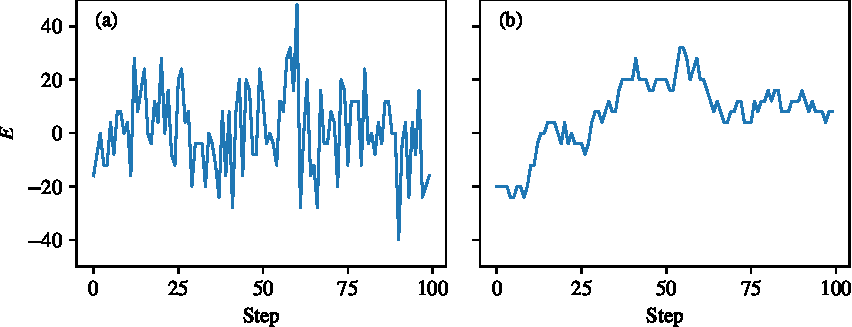
\includegraphics[width=\linewidth]{ch3/rand_autocorr.pdf}
\caption[Energy of Ising model from independent and autocorrelated samples]{
Energies of $100$ samples for the Ising model on the $10 \times 10$ square lattice.
(a) The samples are independently generated from the uniform distribution.
(b) The samples are generated by single-spin updates with $\beta = 0$, thus have autocorrelation.
}
\label{fig:rand-autocorr}
\end{figure}

Although MCMC allows us to estimate the observables from complicated distributions where an exact sampling method cannot be easily constructed, it breaks the assumption of \cref{eq:monte-carlo} that the samples should be independent. In each sampling step, we propose a new configuration $\vs'$ that depends on the current configuration $\vs$, such as flipping a single spin. Moreover, we may reject $\vs'$ and keep using $\vs$ to evaluate the observable for this step. The visual difference between a sequence of independent samples and a Markov chain is shown in \cref{fig:rand-autocorr}. Quantitatively, the samples in the Markov chain $\{\vs^{(1)}, \vs^{(2)}, \ldots, \vs^{(M)}\}$ produce autocorrelation in the observable values~\cite{muller1973dynamic}:
\begin{equation}
C_{O, M}(t) = \left( \frac{1}{M - t} \sum_{i = 1}^{M - t} O\left( \vs^{(i)} \right) O\left( \vs^{(i + t)} \right) \right) - \bbE_\text{MCMC}^2[O],
\end{equation}
where $\bbE_\text{MCMC}[O]$ has the same form as \cref{eq:monte-carlo}, but uses the samples from the Markov chain. We mainly consider the large sample size limit
\begin{equation}
C_O(t) = \lim_{M \to \infty} C_{O, M}(t).
\end{equation}
The correlated samples cause $C_O(t) \neq 0$ when $t > 0$. For example, \cref{fig:autocorr} shows the autocorrelation in energy $C_E(t)$ of the $10 \times 10$ Ising model. As the number of steps $t$ between two samples increases, the average autocorrelation between the two samples decays to zero. At the critical point $\beta_\text{c} = \frac{1}{2} \ln(1 + \sqrt{2}) \approx 0.44$~\cite{onsager1944crystal}, the autocorrelation decays particularly slowly, and we can assume that a sample is approximately independent of the original one only after as many as $10^4$ steps, which renders the MCMC sampling inefficient.

\begin{figure}[htb]
\centering
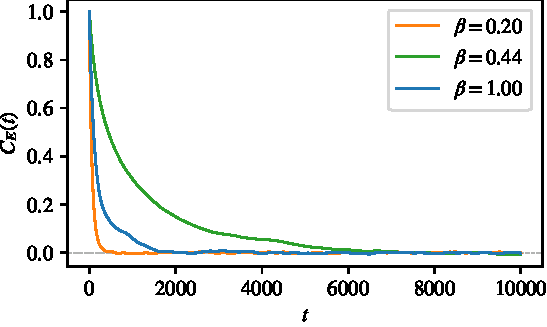
\includegraphics[width=0.7\linewidth]{ch3/autocorr.pdf}
\caption[Autocorrelation in energy for Ising model at different temperatures]{
Autocorrelation in energy $C_E(t)$ of the Ising model on the $10 \times 10$ square lattice at different inverse temperatures $\beta$. The samples are generated by single-spin updates, and the autocorrelation is estimated using $10^7$ samples.
}
\label{fig:autocorr}
\end{figure}

\subsection{Integrated autocorrelation time}

The integrated autocorrelation time~\cite{ambegaokar2010estimating, goodman2010ensemble}, or ``autocorrelation time'' for short, is a metric for MCMC to assess the loss in sample diversity due to autocorrelation, defined by
\begin{align}
\tau = \sum_{t = 1}^\infty r_O(t), \label{eq:iat} \\
r_O(t) = \frac{C_O(t)}{C_O(0)}, \label{eq:rt}
\end{align}
where $r_O(t)$ is the normalized autocorrelation. The value of $\tau$ depends on the complexity of the target distribution, and the method to propose new configurations. It is also known as the relaxation time in analytical studies of the spin dynamics. When estimating it in practice, $C_O(t)$ is replaced by $C_{O, M}(t)$ with a sufficiently large chain length $M$, and we need to verify $M \gg \tau$ after obtaining $\tau$. The summation $\sum_{t = 1}^\infty$ is also replaced by a finite summation $\sum_{t = 1}^{t_\text{cutoff}}$, where $t_\text{cutoff}$ is the first step when $C_{O, M}(t)$ crosses zero~\cite{wu2021unbiased}. It can be efficiently computed using fast Fourier transform (FFT) by the Wiener--Khinchin theorem~\cite{wiener1930generalized}. Other methods to estimate $\tau$ include binning analysis~\cite{wallerberger2018efficient}, and fitting the exponential decay of $C_O(t)$~\cite{bialas2023analysis}. These methods should produce consistent results when the chain length $M$ is sufficiently large.

\begin{figure}[htb]
\centering
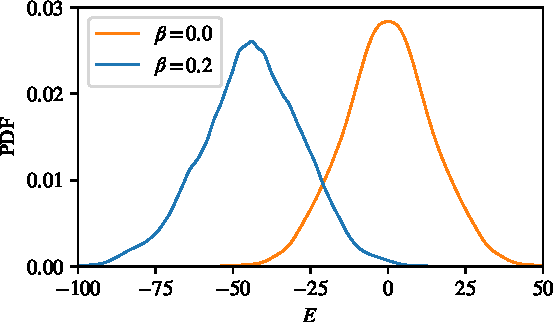
\includegraphics[width=0.7\linewidth]{ch3/energy_hist.pdf}
\caption[Distribution of energy for Ising model at different temperatures]{
Distribution of energy $E$ for the Ising model on the $10 \times 10$ square lattice at inverse temperatures $\beta = 0$ (uniform distribution) and $0.2$ (Boltzmann distribution with moderately high temperature).
The typical energies from the two distributions differ by approximately $50$, and for larger systems and lower temperatures the difference will be even larger, which leads to exponentially low acceptance probability.
The probability density function (PDF) of the distribution is estimated from the samples using Silverman’s method~\cite{silverman1986density}.
}
\label{fig:energy-hist}
\end{figure}

Intuitively, the autocorrelation time takes two factors into account that affect the sample diversity: the correlation between the proposed configuration and the current one, and the acceptance probability. For single-spin updates, the successive samples are almost fully correlated, which leads to high autocorrelation in the observable values. On the other extreme, if we do global updates, i.e., randomly generate a proposed configuration $\vs'$ from the uniform distribution of all configurations in each sampling step, then it is fully uncorrelated with the current one. However, the energy $H(\vs')$ from the uniform distribution is almost always much higher than the current one from the target distribution, as shown in \cref{fig:energy-hist}, which makes the acceptance probability exponentially low, and the collected samples are still almost fully correlated. Between the two extremes of single-spin updates and global updates, a variety of cluster updates have been proposed to balance these two factors, which we will discuss in \cref{sec:cluster-update}.

\subsection{Effective sample size}

The loss in sample diversity is reflected quantitatively in the variance of the Monte Carlo estimator in \cref{eq:monte-carlo-var}. When the Markov chain is in equilibrium, in the presence of autocorrelation, the variance increases to
\begin{equation}
\Var\big[ \bbE_\text{MCMC}[O] \big] = \frac{1}{M_{\text{eff}\,\tau}} \Var[\bar{O}],
\end{equation}
where the effective sample size
\begin{equation}
M_{\text{eff}\,\tau} = \frac{1}{2 \tau + 1} M
\label{eq:eff-sample-size}
\end{equation}
is less than the original sample size $M$.

\section{Critical slowing down}
\label{sec:critical-slow}

\begin{figure}[htb]
\centering
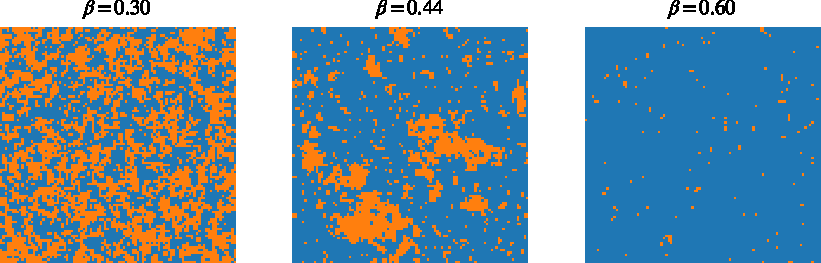
\includegraphics[width=\linewidth]{ch3/ising_samples.pdf}
\caption[Sample of Ising model at different temperatures]{
A typical sample of the Ising model on the $100 \times 100$ square lattice at different inverse temperatures. The blue and the orange plaquettes denote spin up and down respectively. Around the critical point $\beta_\text{c} \approx 0.44$, the clusters of spins are particularly visible, which pose difficulty to MCMC with single-spin updates.
}
\label{fig:ising-samples}
\end{figure}

In many-body systems, the autocorrelation time particularly depends on the physical parameters, such as the inverse temperature $\beta$. It is a long-standing issue with MCMC that the autocorrelation time substantially increases when the system is around its critical point, known as the critical slowing down~\cite{goodman1989multigrid, wolff1990critical}. Intuitively, the collective dynamics of the spins form clusters in the system, which separate from each other by domain walls, as shown in \cref{fig:ising-samples}. Their average diameter is roughly the correlation length $\xi$ of the system. In the case of single-spin update, the Markov chain can be interpreted as a random walk in the configuration space, where it moves from one configuration to an adjacent one with a spin flipped. As a corollary, the time $\tau$ to walk the distance $\xi$ scales by $\tau \sim \xi^2$, regardless of the spatial dimension. Detailed analysis from lattice field theory has shown that $\tau \sim \xi^z$, where $z$ is the dynamical critical exponent, and $z \approx 2$ in many cases~\cite{hohenberg1977theory}. At the critical point, $\xi$ diverges until it is bounded by the system size~\cite{lubetzky2012critical}, therefore the critical slowing down occurs.

From the perspective of statistical complexity~\cite{lopez1995statistical}, the Boltzmann distribution at the critical temperature is difficult to sample from because it has both low entropy and uniformity, which lead to high complexity. It is between the high-temperature distribution with low uniformity but high entropy, and the low-temperature distribution with low entropy but high uniformity. This phenomenon proposes challenge to studies of phase transitions using MCMC, and can be alleviated by cluster updates.

\section{Burn-in stage and Gelman--Rubin statistic}

\begin{figure}[htb]
\centering
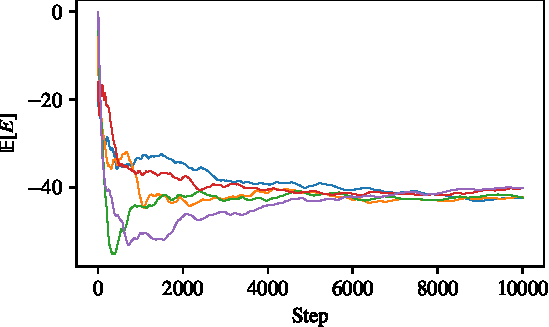
\includegraphics[width=0.7\linewidth]{ch3/multi_chains.pdf}
\caption[Convergence of multiple Markov chains]{
Convergence of five different Markov chains, shown with different colors, for the Ising model on the $10 \times 10$ square lattice at inverse temperature $\beta = 0.2$.
The $y$-axis is the estimated energy using the samples up to the current step.
Although the chains start from different random initializations, they eventually reach the equilibrium distribution and produce consistent estimations of the energy after sufficiently many steps.
}
\label{fig:multi-chains}
\end{figure}

The autocorrelation time $\tau$ is a crucial metric for the efficiency of an MCMC algorithm when the Markov chain is already in equilibrium. However, at the beginning of MCMC, the configuration is usually initialized ``randomly'', which is from the uniform distribution of all configurations. The Markov chain can take many steps to transition from the initial configuration to a typical one in the target distribution, and these steps are called the burn-in or warm-up stage. The untypical samples in this stage introduce bias in the estimation of observables, unless we have exponentially many samples in total to compensate the exponentially low probabilities of untypical samples. To avoid this bias, we discard these samples and start collecting actual samples after this stage.

In theory, the length of the burn-in stage is at most on the order of magnitude of $\tau$, which lets the new configuration decorrelate with the initial one, but in practice we can estimate $\tau$ only if we already know that the burn-in stage has ended. Therefore, we need another metric to estimate the length of the burn-in stage before collecting samples from the equilibrium distribution, which can only be derived from dynamical properties of the Markov chain.

The Gelman--Rubin (GR) statistic~\cite{gelman1992inference, vats2021revisiting} can be used to identify whether the Markov chain has reached the equilibrium. To compute the GR statistic, we generate multiple independent Markov chains starting from different random initial configurations, as shown in \cref{fig:multi-chains}, which is already a common practice to utilize the parallelization capability of modern computers~\cite{lee2010utility}. The samples are denoted by $\vs^{(j, m)}$, where $j \in [1, J]$ identifies the chain and $m \in [1, M]$ identifies the sampling step, and the corresponding observable values are denoted by $O_{j, m} = O\left( \vs^{(j, m)} \right)$. Then we have the mean values
\begin{align}
\bar{O}_j &= \frac{1}{M} \sum_{m = 1}^M O_{j, m}, \\
\bar{O}_* &= \frac{1}{J} \sum_{j = 1}^J \bar{O}_j,
\end{align}
and the variances
\begin{align}
s^2_j &= \frac{1}{M - 1} \sum_{m = 1}^M (O_{j, m} - \bar{O}_j)^2, \\
s^2_* &= \frac{1}{J} \sum_{j = 1}^J W_j,
\end{align}
where $\bar{O}_j$ is the sample mean of the observable over a chain, $\bar{O}_*$ is the sample mean of all chains, $s^2_j$ is the sample variance of a chain, and $s^2_*$ is the mean of these sample variances. Due to the presence of autocorrelation, each $s^2_j$ underestimates the true variance of the target distribution $\sigma^2$. A correction to this bias is estimated by comparing the means of different chains:
\begin{equation}
\frac{B}{M} = \frac{1}{J - 1} \sum_{j = 1}^J (\bar{O}_j - \bar{O}_*)^2.
\end{equation}
Now the estimated variance is
\begin{equation}
\sigma^2_* = \frac{M - 1}{M} s^2_* + \frac{B}{M}.
\end{equation}

The GR statistic is defined to normalize the correction to the estimated variance:
\begin{equation}
R = \sqrt{\frac{\sigma^2_*}{s^2_*}}.
\end{equation}
It is also related to the effective sample size by
\begin{equation}
R \approx \sqrt{1 + \frac{M}{M_\text{eff}}}.
\end{equation}
If we have enough random Markov chains from different initial configurations, which cover all regions of interest in the configuration space, and converge to similar distributions with mean observable values close to each other, then we can assume that the Markov chains have reached equilibrium. It was originally proposed in Ref.~\cite{gelman1992inference} to use a threshold $R < \delta$, and a common choice is $\delta = 1.1$. According to Ref.~\cite{vats2021revisiting}, practical choices of $\delta$ ranges from $1.003$ to $1.3$, and a more stable estimation of the true variance can be obtained from batch-wise variances in the chains.

\section{Other sampling methods}
\label{sec:more-sampling}

\subsection{Importance sampling}
\label{sec:importance-sampling}

Apart from the exact sampling and the MCMC sampling, there are other sampling methods to estimate the observable in \cref{eq:cl-obs}. In principle, we can generate samples $\{\vs^{(1)}, \vs^{(2)}, \ldots, \vs^{(M)}\}$ from any distribution $q(\vs)$, then estimate the observable by
\begin{align}
\bbE_\text{imp}[O] &= \frac{\sum_{i = 1}^M w\left( \vs^{(i)} \right) O\left( \vs^{(i)} \right)}{\sum_{i = 1}^M w\left( \vs^{(i)} \right)}, \label{eq:importance-sampling} \\
w\left( \vs^{(i)} \right) &= \frac{p\left( \vs^{(i)} \right)}{q\left(\vs^{(i)} \right)},
\end{align}
given that $q(\vs)$ has a wider support than $p(\vs)$, i.e., $q(\vs) > 0$ for all $\vs$ such that $p(\vs) > 0$. The probabilities $p(\vs)$ and $q(\vs)$ can be unnormalized, as an overall coefficient in $w(\vs)$ will cancel out in the numerator and the denominator of $\bbE_\text{imp}[O]$. This method is called importance sampling in statistics~\cite{kloek1978bayesian, bugallo2017adaptive}, and the distribution $q(\vs)$ is called an ansatz\footnote{The word ``ansatz'' is borrowed from German. Its plural form is ``Ansätze'' in German, but the adapted form ``ansatzes'' is also used in English literature.} in the context of statistical physics. The ansatz should be close to $p(\vs)$, and easier to sample from than $p(\vs)$. Some choices of the ansatz for importance sampling will be discussed in \cref{sec:nmf}. The variance of this estimator is
\begin{equation}
\Var\big[ \bbE_\text{imp}[O] \big] = \frac{1}{M_{\text{eff}\,w}} \Var[\bar{O}],
\label{eq:importance-sampling-var}
\end{equation}
where the effective sample size
\begin{equation}
M_{\text{eff}\,w} = \frac{\Big( \sum_{i = 1}^M w\left( \vs^{(i)} \right) \Big)^2}{\sum_{i = 1}^M w^2\left( \vs^{(i)} \right)}.
\label{eq:eff-sample-size-w}
\end{equation}
The variance reaches its minimum when $q(\vs) = p(\vs)$, which is in accordance with the intuition that $q(\vs)$ should be as close to $p(\vs)$ as possible.

\subsection{MCMC importance sampling}

Besides reweighing the samples from $q(\vs)$ using the target distribution $p(\vs)$, we can also use the Metropolis--Hastings algorithm in \cref{eq:metropolis} to reject the samples, which we refer to as MCMC importance sampling~\cite{liesenfeld2008improving, schuster2020markov}. In each sampling step, we propose a new configuration $\vs'$ from the distribution $q(\vs')$, which is independent of the current configuration $\vs$, i.e., the proposal distribution $g(\vs' \mid \vs) = q(\vs')$. Then the acceptance probability becomes
\begin{equation}
A(\vs \to \vs') = \min\left( 1, \frac{p(\vs') q(\vs)}{p(\vs) q(\vs')} \right),
\label{eq:mcmc-importance}
\end{equation}
which is close to $1$ if $q(\vs)$ is close to $p(\vs)$. Moreover, this method also reduces the correlation between $\vs$ and $\vs'$ compared to the single-spin update, which leads to the overall reduction of the autocorrelation time. An empirical comparison of the importance sampling and the MCMC importance sampling will be presented in \cref{sec:ncus}. More advanced methods have been proposed to construct the proposal distribution $g(\vs' \mid \vs)$ depending on the current configuration $\vs$, such as the Langevin Monte Carlo~\cite{rossky1978brownian} and the Hamiltonian Monte Carlo~\cite{duane1987hybrid}.

\subsection{Cluster update}
\label{sec:cluster-update}

A variety of cluster update algorithms can also be discussed in the framework of MCMC importance sampling. They have originally arisen from studies of the percolation transition in statistical physics and graph theory, or the series expansion of the partition function~\cite{fortuin1972random, leung1991percolation, evertz1993cluster}. A prominent example is the Wolff algorithm~\cite{wolff1989collective} for Ising models with two-body interactions. In each sampling step, it constructs and flips a cluster of spins according to \cref{alg:wolff}. The resulting proposal probability satisfies $g(\vs' \mid \vs) \propto p_\text{B}(\vs')$, so the acceptance probability is always $1$, which makes the Wolff cluster update far more efficient than the single-spin update when it is applicable.

\begin{algorithm}[H]
\caption[Wolff cluster update]{
Wolff cluster update algorithm to construct and flip a cluster of spins, in the MCMC sampling of the Boltzmann distribution of Ising models with two-body interactions.
$\calC$ is the cluster, $\calB$ is a set of spins on the boundary of the cluster, $\beta$ is the inverse temperature, $\partial i$ denotes the neighbors of the site $i$, and \texttt{rand()} generates a random number from the uniform distribution over $[0, 1)$.
}
\label{alg:wolff}
\begin{algorithmic}[1]
\STATE Input the current configuration $\vs$, interactions $\mJ$
\STATE Randomly choose a site $i$, $\calC \gets \{i\}$, $\calB \gets \{i\}$
\WHILE{$\calB \neq \emptyset$}
    \STATE $i \gets$ any site in $\calB$
    \FOR{$j \in \partial i$}
        \IF{$j \notin \calC$ \AND \texttt{rand()} $> \rme^{\,2 \beta J_{i j} s_i s_j}$}
            \STATE $\calC \gets \calC \cup \{j\}$, $\calB \gets \calB \cup \{j\}$
        \ENDIF
    \ENDFOR
    \STATE $\calB \gets \calB \setminus \{i\}$
\ENDWHILE
\FOR{$i \in \calC$}
    \STATE $s_i \gets -s_i$
\ENDFOR
\STATE Output the new configuration $\vs' \gets \vs$
\end{algorithmic}
\end{algorithm}

\section{Mode collapse}
\label{sec:mode-collapse}

Even if we collect effectively independent samples according to the autocorrelation time and the Gelman--Rubin statistic, it can still be questionable whether those samples actually represent the entire target distribution. The target distribution can have multiple modes, where a ``mode'' is defined to be a cluster of configurations $\{\vs_1, \vs_2, \vs_3, \ldots\}$ with high target probabilities $p(\vs_i)$ and high Markov transition probabilities $M_{\vs_j \vs_i}$ in \cref{eq:markov-matrix} between each other. The paths of configurations to transition from one mode to another always encounter energy barriers, whose heights are proportional to the system size, so the probability of visiting different modes is exponentially low. A possible failure of MCMC is the mode collapse, where the Markov chain is seemingly in equilibrium, but actually it is only in ``equilibrium'' within a single mode, and it takes an impractically long time to visit another mode, which leads to bias in the estimation of observables.

\begin{figure}[htb]
\centering
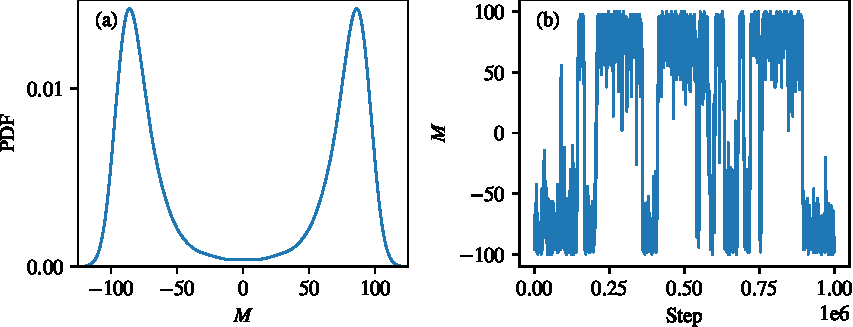
\includegraphics[width=\linewidth]{ch3/mag_hist.pdf}
\caption[Distribution and sampling of magnetization for Ising model]{
(a) Distribution of magnetization $M$ for the Ising model on the $10 \times 10$ square lattice at inverse temperature $\beta = 0.44$.
The two modes characterized by the magnetization are clearly visible.
The energy barrier between the two modes will be even higher as the system size increases, leading to exponentially low probability of transitioning from one mode to another.
The probability density function (PDF) of the distribution is estimated from the samples using Silverman’s method~\cite{silverman1986density}. \\
(b) Magnetizations of samples generated by single-spin updates. The Markov chain can stay in a mode for as long as $10^5$ steps before transitioning to another mode.
}
\label{fig:mag-hist}
\end{figure}

Intuitively, a mode is a peak of the target distribution in the configuration space. Although the exponentially high-dimensional configuration space cannot be directly visualized, we can characterize different modes by appropriate observables, such as the energy or the magnetization, and display the modes as peaks on the histogram of the observable. When the mode collapse happens, the estimated observable characterizing the uncovered modes becomes biased. A typical example is the two modes around the two degenerate ground states $\vs = (+1, +1, +1, \ldots)$ and $\vs = (-1, -1, -1, \ldots)$ in the ferromagnetic Ising model, as shown in \cref{fig:mag-hist}. In this case, even if the estimated energy is still close to the true value in a single mode, the magnetization becomes biased.

The mode collapse in the simple case above can be eliminated by applying the spin flipping symmetry to the generated samples. Other symmetries of the Hamiltonian, such as translations, rotations, and reflections, are also useful to alleviate the mode collapse and improve the accuracy of the estimated observables. Cluster updates are another approach to alleviate this problem, as they can propose large updates to the configuration to transition through the energy barriers that block local updates. The problem becomes more challenging in frustrated models, as discussed in \cref{sec:frustrate}, where the number of degenerate ground states can be exponentially large, and cannot be eliminated by a polynomially large symmetry group~\cite{wannier1950antiferromagnetism, mambrini1999residual, vanderstraeten2018residual}.

The effect of mode collapse is also demonstrated in the context of importance sampling in \cref{eq:importance-sampling}. Assuming the actual distribution of samples $q(\vs)$ only covers a single mode, and is exponentially suppressed in the uncovered modes, where $p(\vs) > 0$ but $q(\vs) \to 0$. Then we have pathologically high $w(\vs)$ in the uncovered modes, which cause the variance in \cref{eq:importance-sampling-var} to diverge. These configurations are identified as the exponentially suppressed configurations (ESCs) in Ref.~\cite{wu2021unbiased}. Even if an estimated observable is still close to the true value in a single mode, the diverging variance indicates that such estimation is unreliable.

\begin{figure}[htb]
\centering
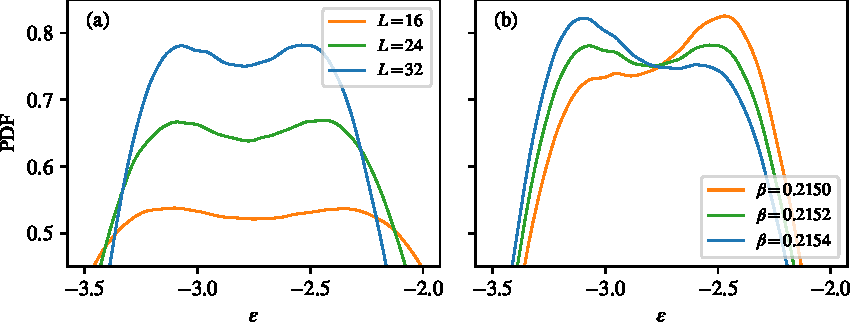
\includegraphics[width=\linewidth]{ch3/fpm_hist_p.pdf}
\caption[Distribution of energy for FPM with different sizes and temperatures]{
Distribution of the energy per site $E / N$ for the FPM in \cref{sec:fpm}.
(a) The results with different system sizes, at their respective ``phase transition'' temperatures where the two peaks have the same area.
(b) The results at different temperatures, with the system size $L = 32$.
The probability density function (PDF) of the distribution is estimated from the samples using Silverman’s method~\cite{silverman1986density}.
The panel (a) is reproduced from Fig.~5 in Ref.~\cite{wu2021unbiased}.
}
\label{fig:fpm-hist-p}
\end{figure}

A particular consequence of mode collapse is the difficulty of MCMC sampling around first-order phase transitions of many-body systems~\cite{binder1987theory}. The first-order phase transition is characterized by a discontinuity in the energy. As an example, we investigate the transition between the ferrimagnetic (fM) and the paramagnetic (PM) phases in the 2D frustrated plaquette model (FPM) in \cref{sec:fpm}, with $N = L \times L$ spins. When we plot its distribution of energies in \cref{fig:fpm-hist-p}, we can see two peaks appearing around the transition temperature. As shown in the panel (a), the depth of the valley between the two peaks grows as the system size $L$ increases, which indicates an increasing energy barrier that blocks local updates. Compared to the peak on the left, the one on the right contains more excited states, but each has lower probability, so the areas of the two peaks are comparable. When the temperature increases, the low-energy peak shrinks while the high-energy one grows, as shown in the panel (b).

The first-order phase transition appears when the two peaks happen to have the same area. In the thermodynamic limit, the probability distribution is exponentially concentrated at the largest peak, so a change of the largest peak causes a discontinuity in the mean energy. Around the phase transition temperature, it is difficult for the system to reach thermal equilibrium, and the system can stay in a metastable state, or can be described by a superposition of multiple classical states. This two-peak distribution proposes challenge to MCMC with local updates, and cluster updates are a viable approach to this problem, as we will discuss in \cref{sec:ncus}.

\chapter{Variational method}
\label{ch:cl-var}

The MCMC method in the previous chapter is widely used to compute various observables of many-body systems. However, a limitation is that it is agnostic of the partition function $Z$ in \cref{eq:boltzmann}, therefore it cannot compute quantities that require $Z$ or the normalized probability $p_\text{B}(\vs)$, including the free energy and the entropy. Variants of MCMC have been proposed to compute $Z$, such as the Wang--Landau algorithm~\cite{wang2001efficient, landau2021guide5}. Nevertheless, they involve other issues such as the discretization of energy histogram~\cite{belardinelli2007wang}, which limit their applicable scenarios as well.

A different approach is to track the probability distribution in the framework of variational approximation and statistical inference~\cite{jordan1999introduction, mackay2003information}, which also has deep roots in statistical physics, traced back to mean-field theories~\cite{chaikin1995principles4, zdeborova2016statistical}. We define a trial distribution $q(\vs)$, or the ``ansatz'' in the context of statistical physics, to approximate the target distribution $p(\vs)$. The form of the ansatz is chosen such that the normalized probability $q(\vs)$ can be efficiently computed given a configuration $\vs$, and the distribution can be easier to sample from than $p(\vs)$, or even be analytically summed over in \cref{eq:cl-obs}. Some choices of the ansatz for variational inference will be discussed in \cref{sec:nmf}.

\section{Variational free energy}

To make a good approximation, we want the ansatz $q(\vs)$ to be as close to the target $p(\vs)$ as possible. A natural metric of the distance between two distributions is the Kullback--Leibler (KL) divergence~\cite{kullback1951information}:
\begin{equation}
D_\text{KL}(q \mid\mid p) = \sum_\vs q(\vs) \ln \frac{q(\vs)}{p(\vs)}.
\end{equation}
When $p(\vs)$ is the Boltzmann distribution, we have
\begin{align}
D_\text{KL}(q \mid\mid p_\text{B}) &= \sum_\vs q(\vs) \left( \ln q(\vs) - \ln \frac{\rme^{-\beta H(\vs)}}{Z} \right) \label{eq:kl} \\
&= \beta (F_q - F), \label{eq:kl-fq}
\end{align}
where $F = -\frac{1}{\beta} \ln Z$ is the true free energy, and we define the variational free energy
\begin{equation}
F_q = \sum_\vs q(\vs) F_\text{loc}(\vs),
\label{eq:fq}
\end{equation}
and the local free energy
\begin{equation}
F_\text{loc}(\vs) = \frac{1}{\beta} \ln q(\vs) + H(\vs).
\label{eq:fq-loc}
\end{equation}

Similar to how we have approximated \cref{eq:cl-obs} by \cref{eq:monte-carlo}, the variational free energy in \cref{eq:fq} is also a weighted sum over the distribution $q(\vs)$ with exponentially many terms, and we can estimate it by Monte Carlo sampling:
\begin{equation}
\bbE_\text{MC}[F_q] = \frac{1}{M} \sum_{i = 1}^M F_\text{loc}\left( \vs^{(i)} \right), \quad
\vs^{(i)} \sim q.
\label{eq:fq-monte-carlo}
\end{equation}
This method has close resemblance to the variational Monte Carlo (VMC) method for quantum systems, which we will discuss in the next part, although the term VMC is rarely used in the context of classical systems. It is worth noting that the variational inference requires to evaluate the normalized probability $q(\vs)$, in contrast to MCMC in the previous chapter where the normalization constant cancels out in the derivation of the Markov Chain, as in \cref{eq:metropolis}. Therefore, it is important to choose an ansatz $q(\vs)$ whose probability is tractable.

\section{Minimization of variational free energy}

The ansatz $q(\vs)$ is usually controlled by some parameters $\theta$, which allows us to minimize the KL divergence by varying $\theta$. In \cref{eq:kl-fq}, the $F$ term is independent of $\theta$, so we only need to minimize $F_q$. As the KL divergence is non-negative, the lower bond of $F_q$ among all possible ansatzes is exactly the true free energy $F$, which is desired to compute in many cases. This property is known as the Bogolubov inequality~\cite{bogolubov1966model}. A common practice is to minimize $\beta F_q$ rather than $F_q$ itself, which avoids the singularity of $\frac{1}{\beta}$ in \cref{eq:fq} when $\beta \to 0$.

\subsection{Gradient descent optimizers}
\label{sec:gd}

As $F_q$ is generally a multivariate nonlinear function of $\theta$, its optimization is usually performed by gradient descent (GD)-based algorithms~\cite{curry1944method}. In the naive setting of GD, in each optimization step $t$ we update $\theta$ by
\begin{equation}
\theta_{t + 1} \gets \theta_t - \gamma \left. \nabla F_q \right|_{\theta = \theta_t},
\label{eq:gd}
\end{equation}
where $\nabla F_q = \frac{\partial F_q}{\partial \theta}$ is the gradient vector of the target function, and $\gamma$ is a small positive number called the learning rate. A common challenge in GD is to choose an appropriate magnitude of $\gamma$, such that the optimization is neither unstable nor too slow to converge~\cite{boyd2004convex}. Another challenge is to converge to the global minimum of the target function, rather than to be trapped by local minima and saddle points. It is particularly important in physical problems to accurately find the global minimum. In contrast to typical machine learning problems, such as computer vision where one only seeks for a ``good-looking'' solution that simulates the inaccurate nature of human vision, in physics there is great interest in obtaining quantitative properties to high accuracies. It is even more crucial to identify qualitative properties about the global minimum, such as symmetries of the ground state. This demand poses unique challenges to the optimization algorithms we use~\cite{chen2023efficient, michaud2023precision}.

When estimating the gradient in \cref{eq:gd}, we usually generate a set of random samples $\{\vs^{(1)}, \vs^{(2)}, \ldots, \vs^{(M)}\}$ in each sampling step, rather than sum over the exponentially large space of configurations. This practice is known as the stochastic gradient descent (SGD)~\cite{robbins1951stochastic, bottou1998online}, and the sample size $M$ is also known as the ``batch'' size in machine learning. In the continuous-time limit, SGD is equivalent to the exact gradient flow with an additional Brownian noise~\cite{hu2017diffusion}, and the variance of the noise scales by $O\left( \frac{1}{M} \right)$. This Brownian motion is also equivalent to a simulated annealing, whose equilibrium distribution is a Boltzmann distribution\footnote{Not to be confused with the physical Boltzmann distribution in the space of the configurations $\vs$.} in the space of the parameter $\theta$. In other words, this noise helps the optimizer escape from local minima and saddle points, given an appropriate ratio of the learning rate to the batch size, which explains the successful application of SGD in various non-convex problems.

Many advanced variants of SGD have been proposed in the recent trend of machine learning~\cite{kashyap2022survey}. In particular, the Adam optimizer~\cite{kingma2015adam} has become the most popular among them. It estimates the appropriate learning rate for each parameter by the second moment\footnote{It is the second moment of the norms of each gradient components in the case of complex-valued gradients.} of the gradient, and uses the first moment to improve the convergence, which largely reduces the manual labor to tune the learning rate. Numerous experiments have demonstrated its broad applicability to machine learning problems, although its convergence properties are still debatable in physical problems that require high accuracy.

\subsection{Second-order optimizers}
\label{sec:ngd}

We refer to GD as a first-order optimizer\footnote{Not to be confused with the order of the convergence speed, which is related to the order in the definition of the optimizer, but not always equivalent.}, because it approximates the target function with only the first-order term in the Taylor expansion, which is the gradient. There are also various second-order optimizers that approximate the target function with a quadratic function, and utilize information about the Hessian matrix to precondition the gradient, i.e., to modify the direction and the magnitude of the gradient in order to reduce the condition number of the optimization problem and accelerate the convergence. The second-order optimizers date back to the Newton's method, which updates $\theta$ by
\begin{equation}
\theta_{t + 1} \gets \theta_t - \gamma \left. \mH^{-1} \nabla F_q \right|_{\theta = \theta_t},
\label{eq:newton}
\end{equation}
where $\mH$ is the Hessian matrix of the target function defined by $H_{i j} = \frac{\partial^2 F_q}{\partial \theta_i \partial \theta_j}$. In this case, the learning rate $\gamma$ can be close to $1$ if the target function is close to the quadratic approximation. However, this method can easily become unstable with highly nonlinear target functions, and an interpolation between the first- and the second-order updates is required to enhance the stability, such as the Levenberg--Marquardt algorithm~\cite{levenberg1944method}. Moreover, directly storing $\mH$ requires $O(n_\text{p}^2)$ space, where $n_\text{p}$ is the number of parameters, and directly inverting it requires $O(n_\text{p}^3)$ computation, which are impractical with large numbers of parameters in neural networks. Therefore, modern methods approximate $\mH^{-1}$ with low-rank updates and line searches, such as the conjugate gradient method~\cite{fletcher1964function} and the limited-memory Broyden--Fletcher--Goldfarb--Shanno (L-BFGS) algorithm~\cite{liu1989limited}. Even with these improvements, the use of second-order optimizers is still hardly practical in large-scale machine learning problems, let alone higher-order ones.

When the target function is a KL divergence, a special technique is to replace $\mH$ in \cref{eq:newton} by the Fisher information matrix
\begin{equation}
\mS = \sum_\vs q(\vs) \nabla \ln q(\vs) \left( \nabla \ln q(\vs) \right)^\transpose.
\label{eq:fim}
\end{equation}
While in principle the gradient can be preconditioned by the inverse of any positive definite matrix, the Fisher information matrix is particularly useful, because it is a natural metric in the function space where the KL divergence measures the distance~\cite{martens2020new}. This technique is known as the natural gradient descent (NGD)~\cite{amari1998natural}, and has led another line of research to approximate it, such as the Kronecker factorization (K-FAC)~\cite{martens2015optimizing} and online approximations~\cite{roux2007topmoumoute, ollivier2017true}. We will give more discussions on NGD in the context of quantum problems in \cref{sec:sr}, where the first-order optimizers produce unsatisfactory results and NGD is considered necessary.

\section{Gradient estimator}

The gradient $\nabla F_q$ in \cref{eq:gd} is derived by automatic differentiation (AD)~\cite{baydin2018automatic} in modern software\footnote{Specifically, the technique to derive the gradient of a scalar target function w.r.t.\ many parameters is named backpropagation, or reverse mode AD.}, which can be more accurate and efficient than traditional methods of finite difference, and more error-prone than manually deriving and implementing the gradient. Care should be taken that \cref{eq:fq} involves the distribution $q(\vs)$, which is a function of $\theta$, but this term no longer exists after replacing \cref{eq:fq} by \cref{eq:fq-monte-carlo}, and we cannot take the gradient of this term in the usual way after sampling the configurations in \cref{eq:fq-monte-carlo}. Therefore, we rewrite the gradient of \cref{eq:fq} as
\begin{align}
\frac{\partial F_q}{\partial \theta}
&= \sum_\vs \left( \frac{\partial q(\vs)}{\partial \theta} F_\text{loc}(\vs) + q(\vs) \frac{\partial F_\text{loc}(\vs)}{\partial \theta} \right) \\
&= \sum_\vs \left( q(\vs) \frac{\partial \ln q(\vs)}{\partial \theta} F_\text{loc}(\vs) + q(\vs) \frac{1}{\beta} \frac{\partial \ln q(\vs)}{\partial \theta} \right).
\label{eq:fq-grad-2-terms}
\end{align}
The second term of \cref{eq:fq-grad-2-terms} becomes
\begin{align}
&\phantom{{}={}}\frac{1}{\beta} \sum_\vs q(\vs) \frac{\partial \ln q(\vs)}{\partial \theta} \\
&= \frac{1}{\beta} \sum_\vs \frac{\partial q(\vs)}{\partial \theta} \\
&= \frac{1}{\beta} \frac{\partial}{\partial \theta} \sum_\vs q(\vs).
\end{align}
As we have the normalization $\sum_\vs q(\vs) = 1$, this term is always zero. The remaining first term of \cref{eq:fq-grad-2-terms} can be again estimated by Monte Carlo sampling:
\begin{equation}
\bbE_\text{MC}\left[ \frac{\partial F_q}{\partial \theta} \right]
= \frac{1}{M} \sum_{i = 1}^M F_\text{loc}\left( \vs^{(i)} \right) \frac{\partial \ln q\left( \vs^{(i)} \right)}{\partial \theta}, \quad
\vs^{(i)} \sim q.
\label{eq:fq-grad}
\end{equation}
This method is called the REINFORCE gradient~\cite{williams1992simple} or the policy gradient~\cite{sutton1999policy} in the context of machine learning, and the gradient of the log-probability $\frac{\partial \ln q(\vs)}{\partial \theta}$ is called the score function~\cite{fisher1935detection, hyvarinen2005estimation, mohamed2020monte}. This kind of differentiation through discrete variables and stochastic sampling of distributions is a recent interest in AD frameworks~\cite{krieken2021storchastic, arya2022automatic, catumba2023stochastic}.

Moreover, a common practice is to shift the terms in the above gradient estimator to have zero means:
\begin{align}
\bbE_\text{MC}\left[ \frac{\partial F_q}{\partial \theta} \right]
&= \frac{1}{M} \sum_{i = 1}^M \left( F_\text{loc}\left( \vs^{(i)} \right) - \tilde{F} \right) \left( \frac{\partial \ln q\left( \vs^{(i)} \right)}{\partial \theta} - \tilde{\vD} \right), \quad
\vs^{(i)} \sim q, \label{eq:fq-grad-baseline} \\
\tilde{F} &= \bbE_\text{MC}[F_q], \\
\tilde{\vD} &= \bbE_\text{MC}\left[ \frac{\partial \ln q}{\partial \theta} \right],
\end{align}
and we do not take the gradient of $\tilde{F}$ and $\tilde{\vD}$ w.r.t.\ $\theta$. Although $\tilde{F}$ and $\tilde{\vD}$ do not affect the expectation of the estimator, they reduce the variance of the estimator in many practical cases, and thus improve the convergence of SGD. This technique falls in a broader family of control variate methods to reduce variances~\cite{ranganath2014black, wan2019neural}.

\section{Comparison between MCMC and variational method}
\label{sec:compare-mcmc}

Besides being able to estimate observables that require the partition function, another feature of variational inference in contrast to MCMC is that it always produces an upper bound of the true free energy, as long as the statistical error of Monte Carlo sampling is sufficiently small. This leads to an intuitive way to compare the accuracies of two variational methods: a lower variational free energy indicates a better approximation of the target distribution. However, this also means a systematic bias in the estimated energy. Other estimated observables can contain biases with unknown directions, and a lower variational free energy does not always imply that other estimated observables are more accurate.

Moreover, there is no straightforward way to improve the accuracy of variational inference as the computation budget grows, whether by increasing the number of variational parameters or optimization steps. In contrast, we can always improve the accuracy or the probability to cover all modes in MCMC by increasing the number of samples. Therefore, to obtain unbiased and accurate estimations of observables, we may use a variational ansatz with MCMC importance sampling in \cref{eq:mcmc-importance}.

In classical statistical physics, certain variational ansatzes have been constructed for specific physical systems, such as variants of the Heisenberg model~\cite{tsallis1976classical, castro2007free, carvalho2012variational}. However, before neural networks became popular, it had been difficult to construct ansatzes that are generalizable to more complicated systems and expressive enough to capture the rich variety of their physical properties. In the following, we discuss some commonly used ansatzes for classical spin systems. They may be easier to sample from than the target Boltzmann distribution, thus can be applied with MCMC importance sampling in \cref{eq:mcmc-importance}; or they may support efficient evaluation of the normalized probability, which is crucial for variational inference in \cref{eq:fq}.

\section{Variational ansatzes for classical spin systems}

\subsection{Naive mean-field ansatz}
\label{sec:nmf}

In the mean-field approach, we construct an approximated Hamiltonian in which all spins are independent. The original interactions between the spins are represented by the ``mean fields'' interacting with the spins, which are not summed over when evaluating the observables. An early practice of this approach was applied to the Curie--Weiss model~\cite{weiss1907hypothese}, which is able to describe the phase transition of ferromagnets. Here we review its derivation and reformulate it in the framework of variational inference.

The Hamiltonian in \cref{eq:cl-ising} can be written as the sum of each spin $s_i$ in its local magnetic field $h_{\text{loc}\,i}$ produced by adjacent spins:
\begin{align}
H(\vs) &= J \sum_{\langle i, j \rangle} s_i s_j
= \frac{1}{2} J \sum_i h_{\text{loc}\,i} s_i, \\
h_{\text{loc}\,i} &= \sum_{j \in \partial i} s_j,
\end{align}
where $\partial i$ denotes the set of nearest neighbors of the site $i$. To find an ansatz whose free energy can be analytically studied, we start from replacing $h_{\text{loc}\,i}$ by an approximate mean field produced by all spins:
\begin{equation}
h_{\text{loc}\,i} \approx h_\text{MF} = \frac{2 d}{N} \sum_i s_i,
\end{equation}
where $d$ is the average number of interactions per site, and each site has $2 d$ nearest neighbors. Then the locally interacting model becomes a globally interacting mean-field model
\begin{equation}
H(\vs) \approx H_\text{MF}(\vs) = \frac{d J}{N} \sum_{i j} s_i s_j.
\label{eq:ham-mf}
\end{equation}

Next, we split each spin variable into $s_i = m + \Delta s_i$, where $m$ is the mean magnetization, $\Delta s_i$ is the fluctuation around the mean, and we assume $|\Delta s_i| \ll |m|$. Then \cref{eq:ham-mf} becomes
\begin{align}
H_\text{MF}(\vs) &= \frac{d J}{N} \sum_{i j} (m + \Delta s_i) (m + \Delta s_j) \\
&= d J m \sum_i (m + 2 \Delta s_i) + \calO(\Delta s^2) \\
&= d J m \sum_i (2 s_i - m) + \calO(\Delta s^2).
\end{align}
Ignoring the higher-order terms $\calO(\Delta s^2)$, the mean-field model can be written in a non-interacting form:
\begin{align}
H_\text{MF}(\vs) &= \sum_i H_{\text{MF}\,i}(s_i), \\
H_{\text{MF}\,i}(s_i) &= d J m (2 s_i - m).
\label{eq:ham-mf-noninter}
\end{align}
Thus we can perform the summation of the partition function:
\begin{equation}
Z_\text{MF}
% = \sum_\vs \rme^{-\beta H_\text{MF}(\vs)}
= \left( \sum_s \rme^{-\beta H_{\text{MF}\,i}(s)} \right)^N
= \left( \rme^{d \beta J m^2} \cdot 2 \cosh (2 d \beta J m) \right)^N.
\end{equation}
The free energy is
\begin{equation}
F_\text{MF} = -\frac{1}{\beta} \ln Z_\text{MF} = - \frac{N}{\beta} \left(d \beta J m^2 + \ln \left( 2 \cosh (2 d \beta J m) \right) \right).
\label{eq:fe-mf}
\end{equation}

At this point, the mean-field free energy $F_\text{MF}$ is derived from the approximated Hamiltonian in \cref{eq:ham-mf}, and we have no guarantee that it is an upper bound of the true free energy derived from the original Hamiltonian in \cref{eq:cl-ising}. However, \cref{eq:kl-fq} still motivates us to minimize $F_\text{MF}$, and the tunable parameter $\theta$ is $m$ here. When $F_\text{MF}$ reaches its minimum, we have the self-consistent equation
\begin{equation}
\frac{\partial F_\text{MF}}{\partial m} = 0 \implies
m + \tanh(2 d \beta J m) = 0.
\label{eq:cw}
\end{equation}
As shown in \cref{fig:cw-tanh}, non-zero solutions to \cref{eq:cw} appear only when $2 d \beta J < -1$, where $J < 0$ and the critical temperature $T_\text{c} = \frac{1}{\beta_\text{c}} = 2 d (-J)$. Therefore, at low temperatures $T < T_c$, the system is ferromagnetic with spontaneous magnetization as the non-zero solutions of \cref{eq:cw}; otherwise, at high temperatures $T > T_c$, the system is paramagnetic without spontaneous magnetization.

\begin{figure}[htb]
\centering
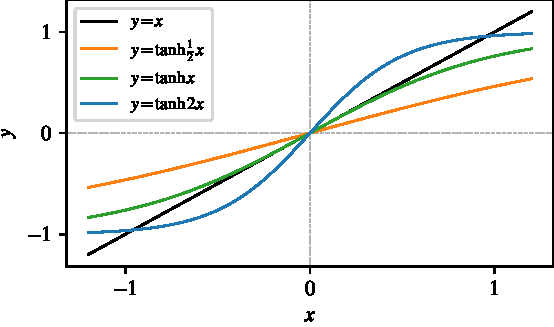
\includegraphics[width=0.7\linewidth]{ch4/cw_tanh.pdf}
\caption[Graphical solution to Curie--Weiss self-consistent equation]{
Graphical solution to the Curie--Weiss self-consistent equation in \cref{eq:cw}, where $x = -m$. The equation $x = \tanh a x$ has non-zero solutions only when $a = 2 d \beta (-J) > 1$.
}
\label{fig:cw-tanh}
\end{figure}

The non-interacting Hamiltonian \cref{eq:ham-mf-noninter} also implies that the joint probability $p(\vs)$ can be factorized into univariate probabilities:
\begin{align}
p_\text{MF}(\vs) &= \prod_i p_{\text{MF}\,i}(s_i), \\
p_{\text{MF}\,i}(s_i) &= \frac{\rme^{-\beta H_{\text{MF}\,i}(s_i)}}{\sum_s \rme^{-\beta H_{\text{MF}\,i}(s)}}.
\end{align}
Simplifying $p_\text{MF}(s_i)$ with \cref{eq:cw}, we have
\begin{equation}
p_\spinup = p_{\text{MF}\,i}(s_i = +1) = \frac{1 + m}{2}, \quad
p_\spindown = p_{\text{MF}\,i}(s_i = -1) = \frac{1 - m}{2}.
\label{eq:p-mf}
\end{equation}
The probability distribution $p_\text{MF}(\vs)$ can serve as a variational ansatz with a single tunable parameter $m$, which we refer to as the naive mean-field (NMF) ansatz.

Next, we use the NMF ansatz and the original Hamiltonian in \cref{eq:cl-ising} to evaluate the variational energy. The energy can be directly evaluated by
\begin{align}
E_\text{MF} &= \sum_\vs p_\text{MF}(\vs) H(\vs) \\
&= N d J (p_\spinup p_\spinup - p_\spinup p_\spindown - p_\spindown p_\spinup + p_\spindown p_\spindown) \\
&= N d J m^2, \\
\shortintertext{and the entropy is}
S_\text{MF} &= -\sum_\vs p_\text{MF}(\vs) \ln p_\text{MF}(\vs) \\
&= -N (p_\spinup \ln p_\spinup + p_\spindown \ln p_\spindown).
\end{align}
Under this ansatz, the free energy $F_\text{MF} = E_\text{MF} - \frac{1}{\beta} S_\text{MF}$ is the same as \cref{eq:fe-mf} derived from the approximated Hamiltonian. It is indeed an upper bound of the true free energy, as it is now derived from the variational ansatz on the original Hamiltonian. For more complicated models on non-regular graphs and with more than two-body interactions, where a self-consistent equation like \cref{eq:cw} cannot be easily constructed, we can still apply the NMF ansatz to obtain a preliminary variational approximation.

\subsection{Bethe ansatz}
\label{sec:bethe}

Starting from an analytical solution to the 1D quantum Heisenberg model~\cite{bethe1931theorie}, the Bethe ansatz has become a gross term for methods to exactly solve or approximate partition functions on lattices and other graphs~\cite{baxter1995solvable, caravelli2022some, gujrati1995bethe, mezard2001bethe}. It is also deeply related to the belief propagation, a message passing algorithm used in Bayesian inference and the recent trend of graph machine learning~\cite{yedidia2003understanding, ikeda2004stochastic}. Unlike the NMF ansatz which approximates the original model using only uniform global interactions, the Bethe ansatz utilizes the local geometry to more accurately represent interactions between nearest neighbors.

In general, the Bethe ansatz is applicable to any probability distribution defined on a graph $\calG = (\calV, \calE)$, where $\calV$ is the set of sites and $\calE$ is the set of edges, as long as the probability of each configuration can be factorized into two-body interactions:
\begin{equation}
p(\vs) = \frac{1}{Z} \prod_{(i, j) \in \calE} f_{i j}(s_i, s_j).
\end{equation}
For the Ising model in \cref{eq:cl-ising}, we have
\begin{equation}
f_{i j}(s_i, s_j) = \rme^{-\beta J s_i s_j}.
\end{equation}

To study the properties of an edge or a site while marginalizing the rest of the graph, we define the auxiliary probability with an edge $(i j)$ removed from the graph:
\begin{align}
\mu^{(i j)}(\vs) &= \frac{1}{Z^{(i j)}} \prod_{(k, l) \in \calE \setminus (i j)} f_{k l}(s_k, s_l), \\
\shortintertext{and with all edges on the site $i$ removed from the graph:}
\mu^{(i)}(\vs) &= \frac{1}{Z^{(i)}} \prod_{(k, l) \in \calE, i \notin \{k, l\}} f_{k l}(s_k, s_l),
\end{align}
where $Z^{(i j)}$ and $Z^{(i)}$ are corresponding normalization constants. We also evaluate the marginal probabilities
\begin{align}
\mu^{(i j)}_i(s_i) &= \sum_{\vs_{\calV \setminus i}} \mu^{(i j)}(s_i, \vs_{\calV \setminus i}), \\
\mu^{(i j)}_{i j}(s_i, s_j) &= \sum_{\vs_{\calV \setminus \{i, j\}}} \mu^{(i j)}(s_i, s_j, \vs_{\calV \setminus \{i, j\}}), \\
\mu^{(i)}_{\partial i}(\vs_{\partial i}) &= \sum_{\vs_{\calV \setminus \partial i}} \mu^{(i)}(\vs_{\partial i}, \vs_{\calV \setminus \partial i}),
\end{align}
where $\partial i = \left\{ j \mid (i, j) \in \calE \right\}$ denotes the neighbors of the site $i$. The univariate marginal probability with an edge removed is denoted by the ``message'':
\begin{equation}
\mu_{i \to j}(s_i) = \mu^{(i j)}_i(s_i).
\end{equation}
After removing the edge $(i, j)$, there is no interaction between $i$ and $j$ after marginalizing other sites, so we have
\begin{equation}
\mu^{(i j)}_{i j}(s_i, s_j) = \mu_{i \to j}(s_i) \mu_{j \to i}(s_j).
\end{equation}

Then we write down the relation between $\mu^{(i j)}(\vs)$ and $\mu^{(i)}(\vs)$. Temporarily ignoring the normalization constants, we can marginalize $\mu^{(i j)}(\vs)$ by first marginalizing $\mu^{(i)}(\vs)$ and then evaluating the remaining interactions between $i$ and $\partial i \setminus j$:
\begin{equation}
\mu^{(i j)}_{i j}(s_i, s_j) \propto \sum_{\vs_{\partial i \setminus j}} \mu^{(i)}_{\partial i}(s_j, \vs_{\partial i \setminus j}) \prod_{k \in \partial i \setminus j} f_{i k}(s_i, s_k).
\end{equation}
It is proposed to approximate the environment to the site $i$ by the product of messages:
\begin{equation}
\mu^{(i)}_{\partial i}(\vs_{\partial i}) \approx \prod_{j \in \partial i} \mu_{j \to i}(s_j).
\label{eq:bethe-prob}
\end{equation}
Now we have the self-consistent equations
\begin{align}
\mu_{i \to j}(s_i) &\propto \sum_{\vs_{\partial i \setminus j}} \prod_{k \in \partial i \setminus j} \mu_{k \to i}(s_k) \prod_{k \in \partial i \setminus j} f_{i k}(s_i, s_k) \\
&= \prod_{k \in \partial i \setminus j} \sum_{s_k} f_{i k}(s_i, s_k) \mu_{k \to i}(s_k),
\label{eq:bethe-message}
\end{align}
from which we can solve the $4 N d$ variables $\mu_{i \to j}(s_i)$. After recovering the normalization constants in \cref{eq:bethe-message}, they can be solved by iterative algorithms if convergence conditions are satisfied~\cite{mooij2007sufficient}, or by gradient-based algorithms.

Given the messages, we can obtain the two-body marginals of the original distribution
\begin{equation}
\mu_{i j}(s_i, s_j) = \frac{f_{i j}(s_i, s_j) \mu_{i \to j}(s_i) \mu_{j \to i}(s_j)}{\sum_{s'_i, s'_j} f_{i j}(s'_i, s'_j) \mu_{i \to j}(s'_i) \mu_{j \to i}(s'_j)},
\end{equation}
and estimate the energy and other observables with at most two-body interactions. For the Ising model in \cref{eq:cl-ising}, we have
\begin{equation}
E_\text{Bethe} = J \sum_{\langle i, j \rangle} \mu_{i j}(s_i, s_j) s_i s_j.
\end{equation}
We can also construct a Bethe entropy from the edge terms and the site terms:
\begin{align}
S_\text{Bethe} &= S_\calE + S_\calV, \\
S_\calE &= -\sum_{(i, j) \in \calE} \ln \sum_{s_i, s_j} f_{i j}(s_i, s_j) \mu_{i \to j}(s_i) \mu_{j \to i}(s_j), \\
S_\calV &= \sum_i \ln \sum_{s_i} \prod_{j \in \partial i} \sum_{s_j} f_{i j}(s_i, s_j) \mu_{j \to i}(s_j),
\end{align}
and the Bethe free energy $F_\text{Bethe} = E_\text{Bethe} - \frac{1}{\beta} S_\text{Bethe}$.

When the graph is a tree, including a 1D chain, there actually exists a probability distribution $p_\text{Bethe}(\vs)$ that produces the marginals $\mu_{i j}(s_i, s_j)$ and the energy $E_\text{Bethe}$, and its entropy is exactly $S_\text{Bethe}$, so the Bethe ansatz can serve as a variational ansatz. For general graphs, however, $S_\text{Bethe}$ no longer equals the entropy of $p_\text{Bethe}(\vs)$, so $F_\text{Bethe}$ is not guaranteed to be an upper bound of the true free energy. Nevertheless, it is a close approximation in many cases. Similar techniques have been generalized to systems beyond two-body interactions, known as cluster variation methods~\cite{pelizzola2005cluster}.

\section{Neural network ansatzes}
\label{sec:nn}

Neural networks, in the context of modern machine learning, are a diverse class of mathematical functions that are historically inspired by the functionality of biological neural networks~\cite{mackay2003information, goodfellow2016deep}. A sharp difference from the previous ansatzes is that neural networks typically have numerous parameters, where the modern large models have reached hundreds of billions of parameters~\cite{brown2020language}. In theory, they are universal approximators of any well-behaved functions if optimized w.r.t.\ the parameters~\cite{hornik1989multilayer}. Although the ideal optimization of so many parameters is intractable in practice, they can still be far more expressive than traditional function approximators~\cite{sontag1998vc}. On the other hand, the large number of parameters makes them more computationally expensive than traditional approaches, and they are usually executed on graphics processing units (GPUs) and other specialized hardware~\cite{chen2020survey}. The optimization of these parameters is known as ``training'' or ``learning'', highlighting the paradigmatic difference from the traditional optimization problems with few variables.

Since their breakthrough on image classification problems~\cite{krizhevsky2012imagenet}, the neural networks with deep multilayer architectures have opened a new era of machine learning studies, known as the ``deep learning''~\cite{goodfellow2016deep}. They have achieved state-of-the-art results in all machine learning domains, and led to a growth of the data-driven paradigm in vast scientific fields~\cite{montans2019data}. The prominent examples including the modeling of languages~\cite{brown2020language}, images~\cite{rombach2022high}, and strategic games~\cite{silver2016mastering}. These successful results are conjectured to stem from the high efficiency of neural networks to represent complicated probability distributions in exponentially high-dimensional spaces --- probabilities of valid speeches in the space of many words, probabilities of recognizable images in the space of many pixels, and probabilities of winning moves in the space of many game board states. Therefore, they have also been introduced as promising ansatzes in many-body physics, where such distributions are a central problem.

\subsection{Layers in neural networks}

Neural networks are composed of a common set of functions, known as ``layers'', and the composition can be arbitrarily sophisticated. The basic architecture is the feedforward neural network (FFNN), which is defined by a sequential composition of alternating linear layers and nonlinear activation layers:
\begin{equation}
\vy = (\text{Lin}_1 \circ \text{Act}_1 \circ \text{Lin}_2 \circ \text{Act}_2 \circ \cdots \circ \text{Lin}_{n_\text{l}} \circ \text{Act}_{n_\text{l}})(\vx),
\label{eq:ffnn}
\end{equation}
where $\vx$ is the inputs to the network, $\vy$ is the outputs, $n_\text{l}$ is the number of layers, and $\circ$ denotes function composition. This architecture is sketched in \cref{fig:nn-arch}.

\begin{figure}[htb]
\centering
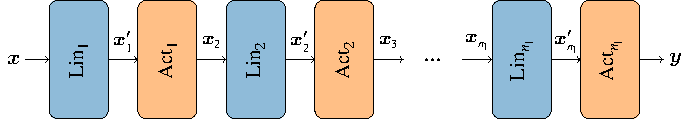
\includegraphics[width=0.9\linewidth]{ch4/nn_arch.pdf}
\caption[Architecture of feedforward neural network (FFNN)]{
Architecture of FFNN, which is a sequential composition of alternating linear layers Lin$_i$ and nonlinear activation layers Act$_i$. Each layer contains its own parameters. The values $\vx_i$ and $\vx'_i$ are outputs from the previous layer, which become inputs to the next layer.
}
\label{fig:nn-arch}
\end{figure}

The linear\footnote{It is technically an affine transformation rather than a linear transformation of $\vx_i$, because $\vb_i$ is included, but the name ``linear layer'' is commonly used in neural networks.} layer is defined by
\begin{equation}
\text{Lin}_i(\vx_i) = \mW_i \vx_i + \vb_i,
\label{eq:linear-layer}
\end{equation}
where $\mW_i$ is called the weight and $\vb_i$ the bias, which are the parameters of this layer. At this point, the parameters are not shared between layers. Assuming $\vx_i$ is a vector of size $n_{\text{in}\,i}$, we can choose an output size $n_{\text{out}\,i}$, then $\mW_i$ is inferred to be a matrix of size $n_{\text{out}\,i} \times n_{\text{in}\,i}$, $\vb_i$ is a vector of size $n_{\text{out}\,i}$, and the input size of the next linear layer $n_{\text{in}\,i + 1}$ equals $n_{\text{out}\,i}$.
In practice, the inputs $\vx_i$ have an additional batch dimension, which denotes evaluating the same network on different input samples, but it is omitted in our discussion for simplicity. The sizes of the intermediate outputs are known as the ``hidden sizes'', and the hyperparameters of the network include the number of layers and the hidden sizes. These hyperparameters, in contrast to the parameters $\mW_i$ and $\vb_i$, define the architecture of the network and mostly determine its expressiveness.

The activation layer, also referred to as the activation function, is an element-wise function of the input vector. A great variety of activation functions has been proposed, each with its own claimed advantages, but most are proven in practice to have only a minuscule impact on the expressiveness of the whole network, apart from the major difference in the output domain~\cite{kunc2024three}. The simplest choice is the rectified linear unit (ReLU):
\begin{equation}
\text{ReLU}(x) = \begin{cases}
x, & x > 0 \\
0, & x \le 0
\end{cases}.
\end{equation}
It has been used since the early research on neural networks, and is still efficient today despite its simplicity.

A modern choice is the Gaussian error linear unit (GELU)~\cite{hendrycks2016gaussian}:
\begin{equation}
\text{GELU}(x) = x\,\Phi(x),
\end{equation}
where $\Phi(x)$ is the cumulative distribution function (CDF) of the unit Gaussian distribution. While having the same asymptotic behaviors at $x \to \pm \infty$ as ReLU, it is derived from the stochastic regularization of the network, and helps stabilize evaluation and training of the network. It is the default choice in NetKet~\cite{carleo2019netket}, and is used in most results reported in this thesis.

In particular, the activation function in the last layer can be the identity function if the outputs are unconstrained in $\bbR$, or specifically constructed to constrain the outputs in an interval. In the latter case, a common choice is the sigmoid function:
\begin{equation}
\text{Sigmoid}(x) = \frac{1}{1 + \rme^{-x}},
\label{eq:sigmoid}
\end{equation}
which maps from $\bbR$ to $(0, 1)$, or to another interval with an additional linear transform. The shapes of ReLU, GELU, and sigmoid are shown in \cref{fig:activations}.

\begin{figure}[htb]
\centering
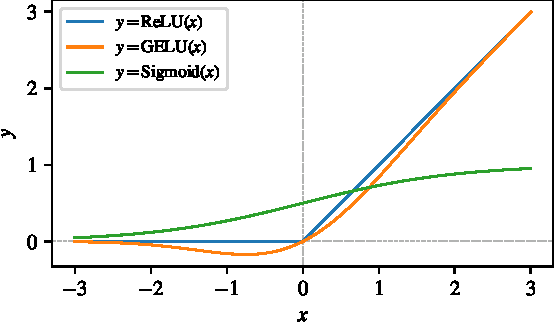
\includegraphics[width=0.7\linewidth]{ch4/nn_activations.pdf}
\caption[Commonly used activation functions in neural networks]{
Commonly used activation functions ReLU, GELU, and sigmoid in neural networks.
Both ReLU and GELU have asymptotic behaviors $y \to 0$ when $x \to -\infty$ and $y \to x$ when $x \to +\infty$, while GELU has more subtle nonlinearity around $x = 0$.
In contrast, the output of sigmoid is bounded in $(0, 1)$.
}
\label{fig:activations}
\end{figure}

\subsection{Symmetries in neural networks: convolutional and pooling layers}

Many-body systems usually have symmetries and locality, which also arise in machine learning of natural images. To take these advantages, the linear layers can be specialized into convolutional layers. Ignoring the layer index, a convolutional layer is denoted by $\vy = \text{Conv}(\vx)$, and in the 1D case it is defined by
\begin{equation}
y_{i, c} = \left( \sum_{k = 1}^{n_\text{k}} \sum_{c' = 1}^{n_\text{c in}} W_{k, c, c'} x_{i + k - 1, c'} \right) + b_{i, c},
\label{eq:conv-layer}
\end{equation}
where $\vx$ is an array of size $n_\text{s} \times n_\text{c in}$, $\vy$ is an array of size $n_\text{s} \times n_\text{c out}$, and we assume that the spatial dimension $n_\text{s}$ is the same in the inputs and the outputs for simplicity. Both the inputs and the outputs have another dimension of ``channels'', also known as ``features'', which determines the size of the network. The convolutional layer acts as if a linear layer on the channel dimension, mapping from $n_\text{c in}$ channels to $n_\text{c out}$ channels. It performs a convolution only on the spatial dimension, rather than the channel dimension. The weights $\mW$ is an array of size $n_\text{k} \times n_\text{c out} \times n_\text{c in}$, where $n_\text{k}$ is the convolution kernel size, and the biases $\vb$ is an array of size $n_\text{k} \times n_\text{c out}$. Higher-dimensional convolutional layers can be defined similarly. In contrast to the convolutional layer, the general linear layer is also known as the dense layer. The FFNN with convolutional layers is known as the convolutional neural network (CNN).

In \cref{eq:conv-layer}, care should be taken when accessing the out-of-boundary values $x_{i, c}$ where $i > n_\text{s}$. For physical systems with open boundary conditions, the common practice is padding with zeros: $x_{i, c} = 0$~\cite{islam2020much}; while for periodic boundary conditions, the convolution can be correspondingly periodic: $x_{i, c} = x_{i - n_\text{s}, c}$. In the latter case, the convolutional layer is translational equivariant in the spatial dimension, which means a translation of the inputs leads to the same translation of the outputs:
\begin{equation}
f(T_d \vx) = T_d f(\vx),
\end{equation}
where $T_d$ denotes the translation by $d$ steps: $T_d (x_1, \ldots, x_{n_\text{s}})$ = $(x_{1 + d}, x_{2 + d}, \ldots, x_{n_\text{s}}, x_1, x_2, \ldots, x_d)$, and $f$ is a neural network composed of convolutional and activation layers. Beyond the translational symmetry, this equivariance can be generalized to more symmetry groups such as rotations and reflections~\cite{luo2021gauge, roth2021group}.

There is also a kind of special linear layers known as pooling layers, which are invariant under the symmetry operations:
\begin{equation}
f(T_d \vx) = f(\vx),
\label{eq:trans-invar}
\end{equation}
where $f$ is a neural network composed of convolutional, activation, and pooling layers. For the purpose of this thesis, we may use the sum pooling as the last linear layer, which sums over the vector input to obtain a scalar output:
\begin{equation}
\text{Pool}(\vx) = \sum_{i = 1}^{n_\text{s}} x_i.
\end{equation}

\subsection{Neural network as variational ansatz}

After introducing the various layers as building blocks, we proceed to apply a neural network as the ansatz for a many-body system of $N$ spins. One may naively define
\begin{align}
q_\theta(\vs) &= \frac{1}{Z} \text{NN}(\vs), \\
Z &= \sum_\vs \text{NN}(\vs),
\end{align}
where NN is a neural network with input size $N$ and a scalar output, and $\theta$ denotes all parameters in it. However, the normalization constant $Z$ is an intractable sum of exponentially many configurations, and this distribution is not easier to sample from than the Boltzmann distribution, therefore it cannot be directly used for MCMC importance sampling in \cref{eq:mcmc-importance}, or for variational inference in \cref{eq:fq}.

Some early attempts have been proposed to choose a simple ansatz which allows efficient cluster updates, such as a two-body interacting Hamiltonian~\cite{liu2017self} or a restricted Boltzmann machine (RBM)~\cite{huang2017accelerated}, and use it in \cref{eq:mcmc-importance}. As the normalization constant of the ansatz is still intractable, thus the variational inference is inapplicable, the parameters of the ansatz are trained in a supervised learning approach. One first generate some samples from the target distribution using traditional MCMC, then optimize the energies of these samples evaluated by the ansatz towards those evaluated by the original Hamiltonian. After training, more samples can be generated from the ansatz using efficient cluster updates. However, the quality of the samples used in training limits the accuracy of this approach.

Another approach is to specifically construct a neural network with tractable normalized probability. A prominent family of such approach is the autoregressive models, which we will discuss in \cref{ch:arnn}. Moreover, a notable family of neural networks with this property are the normalizing flows~\cite{song2017nice, muller2019neural}, which reparameterize the target distribution into a simple one using the same principle as \cref{eq:reparam}. They are mostly used for continuous variables, which are out of the scope of this thesis.

Besides neural networks, tensor networks~\cite{bridgeman2017hand} with chain or tree geometries also supports tractable normalized probability, which we will discuss in \cref{ch:tn}. However, they are more naturally defined and frequently used as variational ansatzes in quantum systems, while in classical systems they are rather usually used to approximate the partition function as a generalization of the transfer matrix to higher dimensions~\cite{verstraete2006criticality, vanderstraeten2018residual, vanhecke2021solving, lanthier2024tensor}.

A lesser-known family of machine learning models sharing this property are the sum-product networks~\cite{poon2011sum}, which define complicated multivariate distributions using directed graphs. They have been applied to various fields of machine learning~\cite{sanchez2022sum}, and they receive renewed attention with the recently proposed Kolmogorov--Arnold networks (KANs)~\cite{liu2024kan}, but their usage is still not as prevalent as neural networks due to limited support in hardware and software~\cite{barham2019machine}.

\chapter{Autoregressive neural networks (ARNNs)}
\label{ch:arnn}

In the previous chapter, we have seen the power of variational inference to approximate the free energy of intractable many-body systems. A crucial requirement for this method is a variational ansatz that supports efficient evaluation of normalized probability and preferably has the rich expressiveness of neural networks. The search for this kind of variational ansatz has led to the development of autoregressive (AR) models, which have yielded the most prominent achievements in modern machine learning, and also found broad applications in many-body physics.

\section{Autoregressive factorization of joint probability}

We start from noticing that any joint probability $q(\vs)$ can be factorized into a product of conditional probabilities:
\begin{align}
q(\vs) &= \prod_i q_i(s_i \mid \vs_{< i}) \label{eq:autoreg} \\
&= q_1(s_1) q_2(s_2 \mid s_1) q_3(s_3 \mid s_1, s_2) \cdots q_N(s_N \mid s_1, s_2, \ldots, s_{N - 1}),
\end{align}
where we still assume that $\vs$ is a vector of $N$ spins, each can take the values $\pm 1$, and $\vs_{< i} = (s_1, s_2, \ldots, s_{i - 1})$ denotes all variables before the $i$-th. This relation between random variables is called an AR model, which is a generalization from the traditional concept of AR in time series, where each random variable only has a linear dependency on the previous ones. In our case, the dependency can be arbitrarily nonlinear.

In principle, if the joint probability is known, one can compute the conditional probabilities by definition:
\begin{equation}
q_i(s_i \mid \vs_{< i}) = \frac{\sum_{\vs_{> i}} q(\vs)}{\sum_{\vs_{\ge i}} q(\vs)},
\end{equation}
which involves summations over exponentially many terms. However, neither do we know the joint probability in practice nor can we exactly perform the summations. We generally parameterize the conditional probabilities by arbitrarily expressive neural networks, therefore the name ARNN, and use variational inference to optimize them towards the target distribution. The requirement of normalization in variational inference is particularly easy to fulfill under this factorization because as long as each conditional probability is normalized: $\sum_{s_i} q_i(s_i \mid \vs_{< i}) = 1$, then the joint probability in \cref{eq:autoreg} will automatically be normalized. For binary variables, each conditional probability is naturally modeled by a Bernoulli distribution $\calB(s_i \mid \hat{s}_i) = (1 - \hat{s}_i) \delta_{s_i, -1} + \hat{s}_i \delta_{s_i, +1}$, which is always normalized and easy to sample from, and the parameter $\hat{s}_i$ can have an arbitrarily sophisticated dependency on the previous variables $\vs_{< i}$.

The joint probability of an AR model supports exact sampling, because we can sample the variables sequentially, following their order defined by the AR model. We first generate the value of $s_1$ from the independent distribution $q_1(s_1)$, then obtain the distribution $q_2(s_2 \mid s_1)$ and generate the value of $s_2$, then obtain the distribution $q_3(s_3 \mid s_1, s_2)$ and so forth, until all variables are generated. This procedure is also known as ancestral sampling. It involves $N$ sequential evaluations of the neural network, which can be a bottleneck in the time complexity of variational inference. On the other hand, when evaluating $q(\vs)$ given all variables $\vs$, all conditional probabilities can be computed in parallel, which is comparatively not a concern in time complexity.

ARNN is an excellent ansatz for variational inference in \cref{eq:fq}, because it supports exact sampling and efficient evaluation of normalized probability, while having the rich expressiveness of neural networks. In the following, we introduce some neural network architectures to parameterize the conditional probabilities, each with its own use cases.

\section{Dense and convolutional ARNNs}
\label{sec:made}

\begin{figure}[htb]
\centering
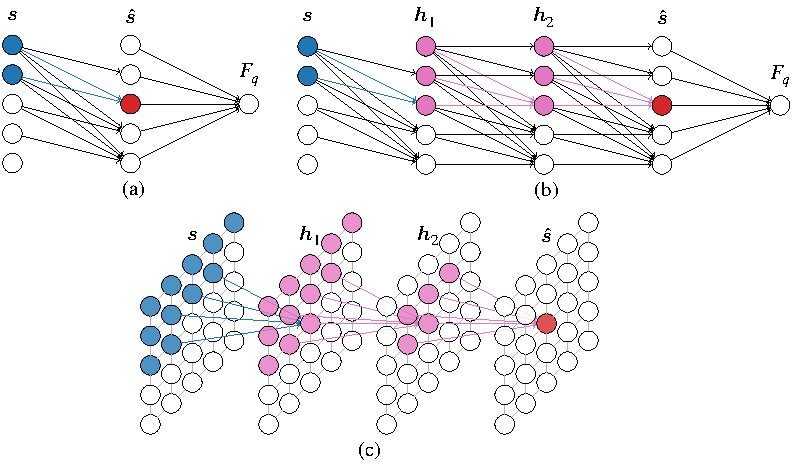
\includegraphics[width=0.9\linewidth]{ch5/arnn_arch.pdf}
\caption[Architectures of autoregressive neural networks (ARNNs)]{
Architectures of dense and convolutional ARNNs for variational inference.
The spins $\vs$ are the inputs to the network.
The values $\hat{\vs}$ are the outputs from the network, which become parameters of the Bernoulli distributions.
The values $\vh_i$ are intermediate results in the network.
The variational free energy $F_q$ is given by \cref{eq:fq}, which depends on both the spins $\vs$ and the parameters $\hat{\vs}$.
The colored sites denote the receptive field of a site in $\hat{\vs}$, i.e., the input and the intermediate sites that an output site depends on.
(a) The network has only one layer, which is densely connected, and masked to ensure the AR property. The connections that are not masked out are illustrated as the arrows.
(b) The network has three masked dense layers.
(c) The network has three masked convolutional layers on a 2D lattice. In each layer, only the connections to one output site are shown for clarity, which depict the shape of the convolution kernel.
This figure is reproduced from Fig.~1 in Ref.~\cite{wu2019solving}.
}
\label{fig:arnn-arch}
\end{figure}

The most general way to parameterize conditional probabilities is a dense feedforward neural network (FFNN) as in \cref{eq:ffnn}, which takes the spins $\vs$ as inputs and outputs the parameters $\hat{\vs}$, then the conditional probabilities are modeled by the Bernoulli distributions $\calB(s_i \mid \hat{s}_i)$. The network needs to fulfill the AR property: each output $\hat{s}_i$ can only depend on the previous inputs $\vs_{< i}$. For a single dense layer, this is achieved by applying a triangular mask on the weight matrix in \cref{eq:linear-layer}:
\begin{gather}
\text{MaskedLin}(\vx) = (\mM \odot \mW) \vx + \vb, \\
M_{i j} = \begin{cases}
1, & i > j \\
0, & i \le j
\end{cases},
\end{gather}
where $\odot$ denotes the element-wise multiplication. This masked linear layer is illustrated in \cref{fig:arnn-arch}~(a). Multiple linear layers can be applied to improve the expressiveness of the network, and only one layer needs to mask out the connections $M_{i i}$, as shown in \cref{fig:arnn-arch}~(b). This architecture is known as the masked autoencoder for distribution estimation (MADE)~\cite{germain2015made}.

Convolutional layers can also be applied to utilize translational symmetry and locality of the physical system, with the same mask $\mM$ to ensure AR property. However, unlike a single convolutional FFNN, the joint probability $q(\vs)$ of a convolutional ARNN is not translational invariant as in \cref{eq:trans-invar}. The ARNN always assigns an artificial order of the spins to factorize the joint probability, thus breaking the translational symmetry. Instead, the purpose of convolutions in ARNN should be understood as enforcing the translational invariance of certain rules to determine the effect of the local environment on a spin.

An early application of 1D convolutional ARNN is the modeling of audios, known as WaveNet~\cite{oord2016wavenet}. The 2D convolutional ARNN has been applied similarly to the modeling of images, known as PixelCNN~\cite{oord2016pixel}, whose shape of the 2D convolutional kernel is illustrated in \cref{fig:arnn-arch}~(c). These ARNN architectures have also been introduced to the modeling of many-body systems, originally under the name of variational autoregressive networks (VANs)~\cite{wu2019solving}, and achieved superior results compared to traditional variational ansatzes.

In addition to dense and convolutional ones, another widely used family of ARNNs is the recurrent neural networks (RNNs), which incorporate the translational symmetry of the physical system in another way. They maintain the AR property by updating of some hidden variables $\vh^{(i)}$, also known as ``memories'', at each AR step $i$:
\begin{align}
\vh^{(i)} &= f\left( s_{i - 1}, \vh^{(i - 1)} \right), \label{eq:rnn-update} \\
\hat{s}_i &= g\left( \vh^{(i)} \right), \label{eq:rnn-output}
\end{align}
where $f$ and $g$ can be arbitrarily sophisticated neural networks, and their parameters are usually shared between sites. Due to the sharing of parameters, RNNs can achieve satisfactory results with fewer parameters than dense networks. More variants of RNNs, including hybrids with CNNs and tensor networks, are also used in practice~\cite{oord2016pixel, khandoker2023supplementing}. In particular, the popular large language models in modern machine learning have essentially inherited the principles of RNN~\cite{brown2020language}. It is also worth mentioning that ARNNs with hierarchical architectures~\cite{bialas2022hierarchical} and representations in frequency or wavelet spaces~\cite{nash2021generating, mattar2024wavelets} have been proposed to enhance translational symmetry and scalability.

\subsection{Numerical results}

\begin{figure}[htb]
\centering
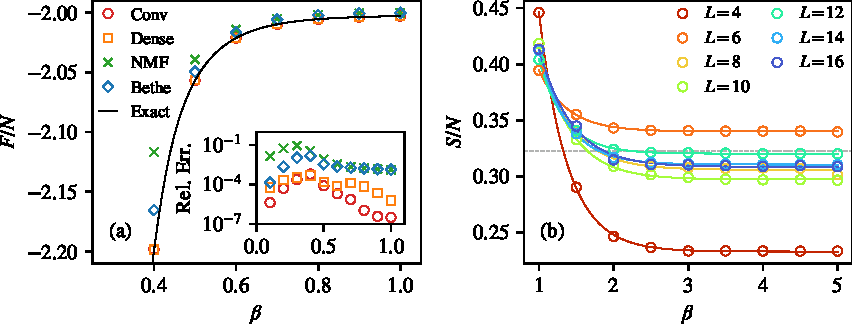
\includegraphics[width=\linewidth]{ch5/arnn_ising.pdf}
\caption[ARNN results of Ising model on square and triangular lattices]{
(a) Free energy per site $F / N$ of the ferromagnetic (FM) Ising model on the $16 \times 16$ square lattice with periodic boundary conditions (PBC), at varying inverse temperature $\beta$, given by a dense ARNN and a convolutional ARNN, compared to the exact result~\cite{onsager1944crystal} and the traditional methods of naive mean-field (NMF) and Bethe ansatzes.
The inset shows the relative error of the numerical results compared to the exact result. \\
(b) Entropy per site $S / N$ of the frustrated antiferromagnetic (AFM) Ising model on triangular lattices of different sizes $N = L \times L$ with PBC, given by a convolutional ARNN.
The curves are least-squares fittings of $S / N = a \rme^{-b \beta} + c$, where $a, b, c$ are parameters for fitting, and $c$ is the residual  entropy when $\beta \to \infty$.
The horizontal dashed line indicates the exact result $\lim_{N \to \infty} \lim_{\beta \to \infty} S / N \approx 0.323$~\cite{wannier1950antiferromagnetism, wannier1973antiferromagnetism, houtappel1950order}.
Note that the curves for $L = 8, 14, 16$ are almost overlapped.
This figure is reproduced from Fig.~2 in Ref.~\cite{wu2019solving}.
}
\label{fig:arnn-ising}
\end{figure}

\subsubsection{Square Ising model}

We first demonstrate the performance of ARNN on the well-studied ferromagnetic (FM) Ising model on the $10 \times 10$ square lattice with periodic boundary conditions (PBC), where the analytical result~\cite{onsager1944crystal} and the traditional methods of naive mean-field (NMF) ansatz in \cref{sec:nmf} and Bethe ansatz in \cref{sec:bethe} are available for comparison. A dense ARNN and a convolutional ARNN are trained on the Boltzmann distribution of this Hamiltonian, whose hyperparameters, such as the number of layers, the number of channels, and the convolution kernel size, are selected to produce the lowest variational free energies within a reasonable computation budget. The networks are trained from scratch at each inverse temperature $\beta = 0.1, 0.2, \ldots, 1$. \Cref{fig:arnn-ising}~(a) shows the results of free energy, where we can clearly see that the ARNNs produce superior results compared to the traditional ansatzes, whose relative errors are lower by orders of magnitude.

In particular, the results from the convolutional ARNN are generally more accurate than those from the dense one with a similar number of parameters, thanks to the utilization of the translational symmetry and the locality of the physical system. This comparison justifies the use of convolutional layers in ARNN, even though the overall joint probability is not translational invariant. However, this advantage diminishes around the critical point $\beta_c = \frac{1}{2} \ln(1 + \sqrt{2}) \approx 0.44$, where the correlation length of the physical system diverges until it is bounded by the system size, as discussed in \cref{sec:iat}. The convolutional neural network can capture these long-range correlations only if the size of its receptive field is at least comparable to the correlation length.

\subsubsection{Triangular Ising model}
\label{sec:arnn-tri-ising}

Then we apply the convolutional ARNN to the more complicated problem of antiferromagnetic (AFM) Ising model on the triangular lattice with PBC, which is geometrically frustrated. As discussed in \cref{sec:frustrate}, frustration leads to exponentially many degenerate ground states and a non-zero residual entropy, which poses challenge for MCMC and previous variational ansatzes. In \cref{fig:arnn-ising}~(b), the ARNN produces entropies that exponentially decay to a constant as $\beta \to \infty$ for each system size $L$, and converge around the analytical result as $L \to \infty$. These results demonstrate the rich expressiveness of ARNN, which has the potential to accurately approximate exponentially complex target distributions using polynomial computation time and number of parameters.

\subsubsection{Hopfield model}
\label{sec:arnn-hop}

\begin{figure}[htb]
\centering
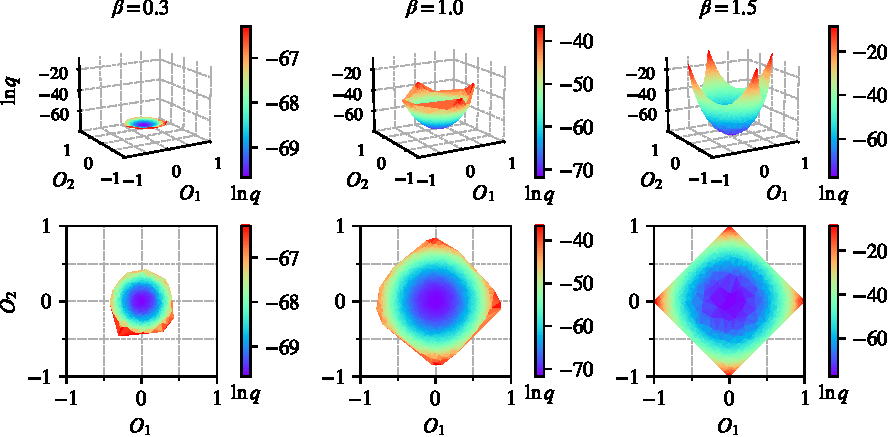
\includegraphics[width=\linewidth]{ch5/arnn_hop.pdf}
\caption[ARNN results of Hopfield model]{
Log-probability $\ln q$ of samples from a dense ARNN, for the Hopfield model with $N = 100$ spins and $n_\text{pat} = 2$ orthogonal patterns.
The top row shows the 3D view of the log-probability surfaces, and the bottom row shows the same results in the 2D view from top.
The columns are results with different inverse temperatures $\beta = 0.3, 1.0, 1.5$.
The $O_1$ and $O_2$ axes denote the overlaps between each sample and the two patterns respectively, as defined in \cref{eq:cl-overlap}.
The four ground states have $(O_1, O_2)$ = $(+1, 0)$, $(-1, 0)$, $(0, +1)$, $(0, -1)$ respectively.
This figure is reproduced from Fig.~3 in Ref.~\cite{wu2019solving}.
}
\label{fig:arnn-hop}
\end{figure}

An experiment to qualitatively study the ability of ARNN to capture multiple ground states is on the Hopfield model in \cref{sec:hopfield}. We construct a Hopfield model with $N = 100$ spins and $n_\text{pat} = 2$ random orthogonal patterns, and train a dense ARNN that consists of only a single layer. Then we generate $10^4$ samples from the ARNN, and compute their probabilities and their overlaps with the two patterns, respectively. \Cref{fig:arnn-hop} shows that the ARNN successfully samples the memorized patterns with exponentially higher probabilities than other states, in the retrieval phase with high $\beta$. This indicates the capability of ARNN to avoid mode collapse and capture all the modes separated by exponentially high energy barriers in this Hamiltonian.

\subsubsection{Sherrington--Kirkpatrick (SK) model}

\begin{figure}[htb]
\centering
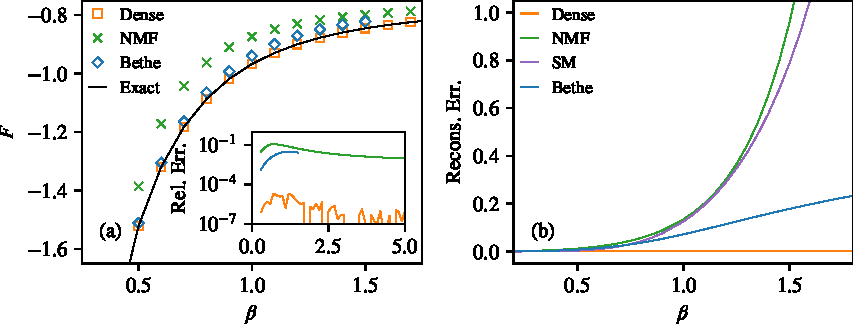
\includegraphics[width=\linewidth]{ch5/arnn_sk.pdf}
\caption[ARNN results of Sherrington--Kirkpatrick (SK) model and inverse SK problem]{
(a) Free energy per site $F / N$ for a random instance of the SK model with $N = 20$ spins, at varying inverse temperature $\beta$, given by a dense ARNN, compared to the exact result by enumeration, the NMF ansatz, and the Bethe ansatz. The inset shows the relative error of the numerical results compared to the exact result.
The iterative solution of the Bethe ansatz converges only when $\beta \le 1.5$. \\
(b) Reconstruction error of the inverse SK problem with $N = 20$ spins, given by a dense ARNN, compared to the NMF ansatz~\cite{roudi2009ising}, the Sessak--Monasson (SM) expansion~\cite{sessak2009small}, and the Bethe ansatz~\cite{ricci2012bethe}.
This figure is reproduced from Fig.~4 in Ref.~\cite{wu2019solving}.
}
\label{fig:arnn-sk}
\end{figure}

We also have the experiment on the Sherrington--Kirkpatrick (SK) model in \cref{sec:sk}, which has frustrated interactions with even higher complexity than the previous models. As a proof of concept, we generate a random instance of the SK model with $N = 20$ spins and compute its properties by exact enumeration. Then we train a dense ARNN with a single layer. \Cref{fig:arnn-sk}~(a) shows that the ARNN still produces a substantially more accurate approximation than traditional ansatzes for this Hamiltonian, especially in the glassy phase with high $\beta$ where the iterative solution of the Bethe ansatz fails to converge.

\subsubsection{Inverse SK problem}

In addition to the ordinary problem of estimating the observables given the Hamiltonian, ARNNs can also be used in the inverse SK problem, where we estimate the unknown interactions $\{J^*_{i j}\}$ given the correlations $\{C^*_{i j}\}$. Because each estimated correlation $\bbE_\text{MC}[C_{i j}]$ as in \cref{eq:monte-carlo} is a differentiable function of $\{J_{i j}\}$, we can directly use stochastic gradient descent to minimize the least-square loss
\begin{equation}
L\left( \{J_{i j}\} \right) = \frac{1}{N^2} \sum_{i j} \left( \bbE_\text{MC}[C_{i j}] - C^*_{i j} \right)^2.
\end{equation}
In this problem, we use an ARNN with two dense layers to estimate $C_{i j}$. The abilities of different methods to estimate the interactions is assessed by the reconstruction error
\begin{equation}
\text{Recons. Err.} = \frac{1}{N^2} \sum_{i j} \left( J_{i j} - J^*_{i j} \right)^2,
\end{equation}
where $J_{i j}$ are the estimated values and $J^*_{i j}$ are the true values. The results are shown in \cref{fig:arnn-ising}~(b), where the ARNN again outperforms traditional methods by a large margin.

\subsection{Remarks on network sizes}

It is worth discussing the sizes of the ARNNs used in the above experiments. For fully connected cases of the Hopfield model, the SK model, and the inverse SK problem, we use small ARNNs containing only $O(N^2)$ parameters, which take minutes to train on a high-end GPU as of this writing, and they produce substantially better results than the Bethe ansatzes with the same order of parameters. However, for the Ising models on the $16 \times 16$ square and triangular lattices, the ARNNs with the optimal variational free energies we have found contain as many as $O(10^6)$ parameters, while the Bethe ansatzes contain only $O(10^3)$. The large number of parameters also leads to substantially more computation time to evaluate the observables, since the training and the sampling of such a large neural network typically take hours on a high-end GPU, while the NMF ansatz and the Bethe ansatz can be solved almost instantly. Therefore, many use cases of neural networks to replace traditional ansatzes appear only in the regime where we seek for much higher accuracy at the cost of correspondingly more computation. The comparison of neural networks and traditional methods under the same computation budget will be discussed in \cref{sec:arnn-mcmc}.

Apart from training a new network with each system size and temperature, it has also been proposed to directly reuse or fine-tune a trained network with different system sizes and temperatures~\cite{efthymiou2019super, mills2019extensive, rende2024fine}. This line of research opens a promising way to numerically compute the renormalization group (RG) flow, and extrapolate the critical temperature to the thermodynamic limit~\cite{ron2002inverse}.

\section{Sparse two-body ARNN (TwoBo)}
\label{sec:twobo}

In the previous section, we have seen that the simple ARNN with dense architecture approximates many-body systems to much higher accuracy than traditional ansatzes, but also introduces much more trainable parameters and requires longer computation time. The convolutional ARNN reaches even higher accuracy with approximately the same number of parameters, as it utilizes the translational symmetry and the locality of the physical system. In this section, we continue to search for a more sophisticated ARNN architecture that further embodies knowledge of the physical system, particularly the sparsity, to reduce the number of trainable parameters and the computation time without losing the expressiveness.

An approach has been proposed in Ref.~\cite{pan2021solving} to convert any many-body system on a sparse graph into an equivalent system on a smaller dense graph using the feedback vertex set. Meanwhile, it has been noticed in Ref.~\cite{pr2021analysis} that the dense ARNN architecture involves a lot of redundant computation that can be eliminated given the physical properties of the Boltzmann distribution and the locally interacting Hamiltonian. In the following, we present a different approach proposed in Ref.~\cite{biazzo2024sparse}, which utilizes these physical properties to improve the efficiency of ARNN.

\subsection{TwoBo architecture from Boltzmann distribution}

We start from directly factorizing the many-body Boltzmann distribution $p_\text{B}(\vs)$ into AR conditional distributions in \cref{eq:autoreg}:
\begin{equation}
p_{\text{B} i}(s_i \mid \vs_{< i})
= \frac{\sum_{\vs_{> i}} p_\text{B}(\vs)}{\sum_{\vs_{\ge i}} p_\text{B}(\vs)}
= \frac{\sum_{\vs_{> i}} \rme^{-\beta H(\vs)}}{\sum_{\vs_{\ge i}} \rme^{-\beta H(\vs)}},
\end{equation}
and simplifying the result. When the Hamiltonian has only two-body interactions, such as the Ising model in \cref{eq:cl-ising-general}, it has been derived in Ref.~\cite{biazzo2024sparse} that the conditional probability takes the form:
\begin{align}
p_{\text{B} i}(s_i = +1 \mid \vs_{<i}) &= S\left( 2 \beta \xi_{i i} + \rho_{\text{B} i}\left( \{\xi_{i l} \mid l > i\} \right) \right), \label{eq:twobo} \\
\xi_{i l} &= \sum_{k < i} J_{k l} s_k, \label{eq:twobo-xi}
\end{align}
in the notations of this thesis, and omitting the external fields for simplicity. Here, $S$ is the sigmoid function in \cref{eq:sigmoid}, and $\rho_{\text{B} i}$ is a function depending on $\mJ$ and $\beta$. The function $\rho_{\text{B} i}$ is different for each index $i$, and it only takes the intermediate variables $\xi_{i l}$ with $l > i$ as the inputs. Although the exact evaluation of $\rho_{\text{B} i}$ can take exponential time, it has been shown in Ref.~\cite{biazzo2023autoregressive} that $\rho_{\text{B} i}$ can be simplified for specific physical systems, such as an analytical expression for the Curie--Weiss model and a replica symmetric breaking (RSB) approximation for the SK model.

\begin{figure}[htb]
\centering
\hspace*{\fill}
\subfloat[]{\raisebox{0.055\linewidth}{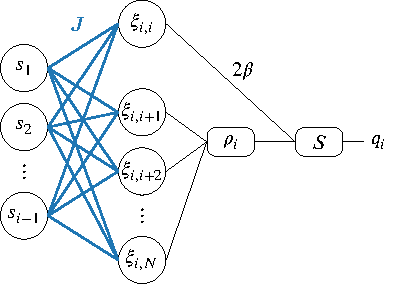
\includegraphics[width=0.4\linewidth]{ch5/twobo_arch.pdf}}}
\hspace*{\fill}
\subfloat[]{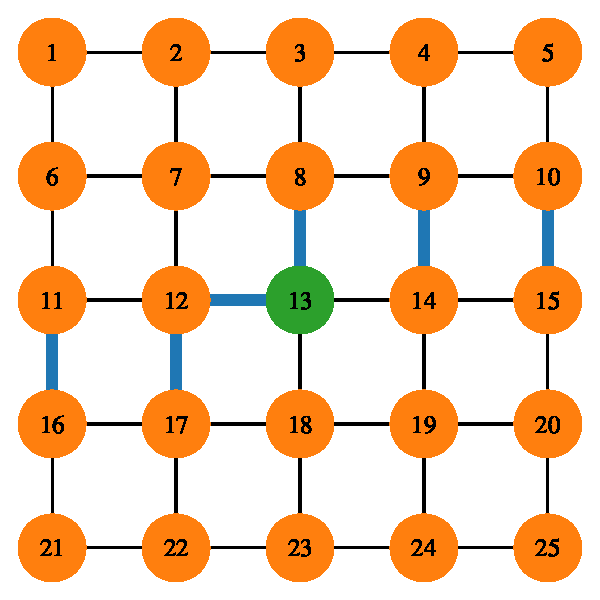
\includegraphics[width=0.4\linewidth]{ch5/twobo_grid_2d.pdf}}
\hspace*{\fill}
\caption[Architecture of the sparse two-body ARNN (TwoBo)]{
(a) Sketch of the TwoBo ARNN architecture to compute a conditional probability $q_i(s_i = +1 \mid \vs_{< i})$.
The weights of the first layer are directly taken from the interaction matrix $\mJ$ and fixed.
The function $\rho_i$ is parameterized by a dense layer, whose inputs are the variables $\{\xi_{i l} \mid l > i\}$ after the first layer.
The last activation function $S$ is the sigmoid function in \cref{eq:sigmoid}, and there is a skip connection from $\xi_{i i }$ to $S$ with the fixed weight $2 \beta$. \\
(b) Calculating the conditional probability $q_i(s_i \mid \vs_{< i})$ with $i = 13$ on a 2D grid of $N = 25$ spins. The edges between the spins $\vs_{< i}$ and $\vs_{\ge i}$ are highlighted in blue, and only these edges are used when computing the intermediate variable $\xi_{i l}$. Therefore, among the variables $\{\xi_{i l} \mid l > i\}$, only those with $l < i + L$ are kept as inputs to $\rho_i$, and the others are ensured to be zero, which enhances the sparsity of the TwoBo network.
This figure is reproduced from Fig.~1 in Ref.~\cite{biazzo2024sparse}.
}
\label{fig:twobo-arch-grid}
\end{figure}

For the purpose of this thesis, we approximate $\rho_{\text{B} i}$ using a neural network $\rho_i$ with trainable parameters, and we have surprisingly found that using a single dense layer is enough to obtain results with satisfactory accuracies in our numerical experiments. In addition, we interpret the linear transformation from the input spins $s_i$ to the intermediate variables $\xi_{i l}$ in \cref{eq:twobo-xi} as another linear layer without bias, whose weights are taken directly from $\mJ$ and are not trained. Therefore, \cref{eq:twobo} becomes an ARNN ansatz $q_i(s_i \mid \vs_{< i})$ as shown in \cref{fig:twobo-arch-grid}~(a). This architecture is colloquially named TwoBo because the authors were tired of the ever-growing lengths of acronyms.

\subsection{Sparsity of intermediate variables}
\label{sec:twobo-sparse}

Incorporating the interaction matrix $\mJ$ into the parameters of TwoBo leads to the opportunity to reduce the computation time and the number of trainable parameters using the sparsity of the physical system. In general, the first layer in \cref{eq:twobo-xi} can be evaluated by a matrix-vector multiplication $\mJ \vs$ while storing cumulative sums, which takes $O(N^2)$ time, where $N$ is the number of spins. When the physical system is sparse and the number of non-zero entries in $\mJ$ only scales by $O(N)$, the evaluation takes only $O(N)$ time as well.

For each function $\rho_i$, there are $N - i$ input variables in general and a scalar output, which introduces $O(N)$ parameters and $O(N)$ computation time when parameterized by a single dense layer. Fortunately, when the physical system has a local geometry, many of the input variables are ensured to be zero. For example, on a 2D grid with $N = L^2$ spins as shown in \cref{fig:twobo-arch-grid}~(b), each variable $\xi_{i l}$ is non-zero only when $i < l < i + L$, therefore the number of input variables to $\rho_i$, the number of parameters in it, and the time to evaluate it are reduced from $O(L^2)$ to $O(L)$. Taking into account all the functions $\{\rho_i \mid 1 \le i \le N\}$, they take $O(L N) = O(L^3)$ time to evaluate in total, which dominates over the $O(N)$ time of the first layer. Those functions also have $O(L^3)$ parameters in total. Therefore, the time to evaluate the TwoBo ansatz and the number of trainable parameters in it scale both by $O(L^3)$, which is polynomially lower than $O(L^4)$ of the dense ARNN (MADE) in \cref{sec:made}. Similarly, the time and the space are reduced from $O(L^6)$ to $O(L^5)$ on 3D grids.

\subsection{Numerical results}
\label{sec:twobo-results}

The performance of TwoBo is demonstrated in numerical experiments using the Edwards--Anderson (EA) model with binary interactions on 2D and 3D grids with PBC, as well as random regular graphs (RRGs). As discussed in \cref{sec:ea}, the EA model is generally more difficult to solve than the simple Ising model in \cref{sec:made}, and the 3D EA model is particularly challenging from the perspective of computational complexity. Moreover, the RRG demonstrates the performance of TwoBo on systems without regular geometry. We use RRGs with degree $d = 3$, and sample them from the uniform distribution of all RRGs with the given $N$ and $d$ using the Steger--Wormald algorithm~\cite{steger1999generating}. Each reported result is averaged over $10$ random instances of the Hamiltonian, and the error bar shows the standard error over the instances.

The results from TwoBo are compared with those from MADE. We use the MADE with only one layer, and it still has more trainable parameters than the TwoBo with the same system size. On the 2D grids, another comparison is made with the RNN architecture in Ref.~\cite{hibat2021variational}, which has outperformed several dense and convolutional ARNN architectures in the regime of numerous parameters. In this thesis, we compare with it mainly in the regime of few parameters, using only four memory units and a comparable number of trainable parameters to TwoBo, while the comparison using more parameters will be shown in \cref{fig:twobo-rnn-param}.

An annealing procedure is performed to compute the free energies at different inverse temperatures $\beta \in (0, 3]$, and to help the optimization converge to the desired global minimum at high $\beta$. We equally divide the range of $\beta$ into $N_\text{anneal} = 60$ annealing steps. At the first $\beta = 0.05$, we perform $N_\text{warm} = 500$ optimization steps as a warm-up. After that, in each annealing step, we perform $N_\text{opt} = 200$ optimization steps while keeping $\beta$ unchanged. In the next annealing step, we continue to optimize the ansatz with a different value of $\beta$. All the architectures of TwoBo, MADE, and RNN are trained using this procedure.

\subsubsection{Variational free energy and ground state energy}

\begin{figure}[htb]
\centering
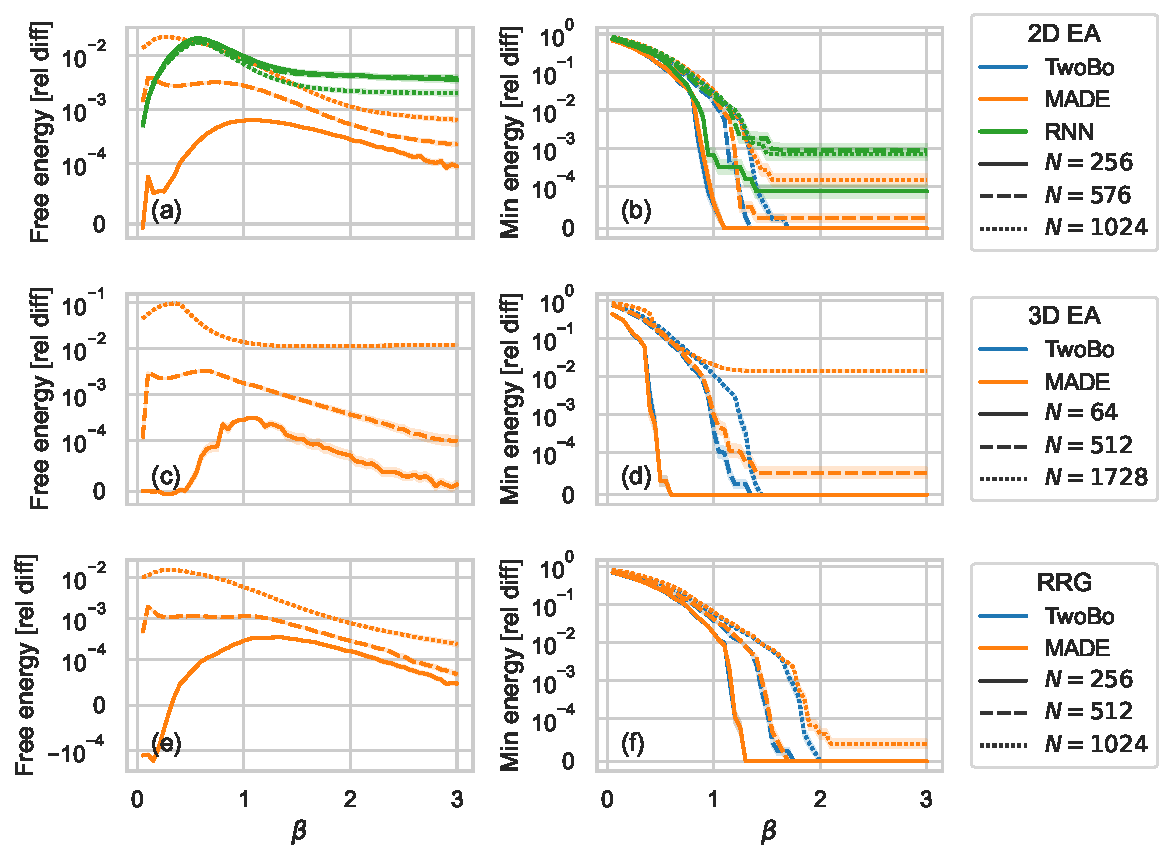
\includegraphics[width=\linewidth]{ch5/twobo_ea.pdf}
\caption[TwoBo results of Edwards--Anderson (EA) model]{
Variational free energy (left column) and minimum energy of sampled configurations (right column) at varying inverse temperature $\beta$, for the EA model on 2D grids (top row), 3D grids (middle row), and RRGs (bottom row) of different sizes.
The performance of TwoBo, MADE, and RNN (only in 2D) architectures are compared.
The variational free energy is shown as the relative difference from TwoBo at the same $\beta$, and the minimum energy is relative from the one found by TwoBo at $\beta = 3$.
The $y$-axis uses the logarithmic scale when the absolute value is greater than $10^{-4}$.
This figure is reproduced from Fig.~2 in Ref.~\cite{biazzo2024sparse}.
}
\label{fig:twobo-ea}
\end{figure}

As shown in the left column of \cref{fig:twobo-ea}, TwoBo gives a lower variational free energy than MADE and RNN with a comparable number of trainable parameters, on almost all tested geometries, system sizes, and temperatures, except in the simple cases of low $\beta$. This demonstrates the accuracy of TwoBo in approximating the Boltzmann distribution, even with disordered and frustrated Hamiltonians, and this advantage becomes more substantial at larger system sizes.

The right column of \cref{fig:twobo-ea} shows the minimum energy found by the ansatzes in the annealing procedure, which is of more interest in combinatorial optimization problems. TwoBo is also able to find energies lower than those of MADE and RNN, especially at large system sizes. In addition to variational methods, we also use the exact solvers in McGroundstate~\cite{charfreitag2022mcsparse} and the heuristic solvers in MQLib~\cite{dunning2018what} to solve the same systems. Compared to these solvers, TwoBo gives equal or lower energies with comparable computation time in all tested cases, which provides evidence that the sophisticated heuristics of neural networks outperform traditional methods in optimization problems with many variables and complicated interactions.

\subsubsection{Convergence of training}

\begin{figure}[htb]
\centering
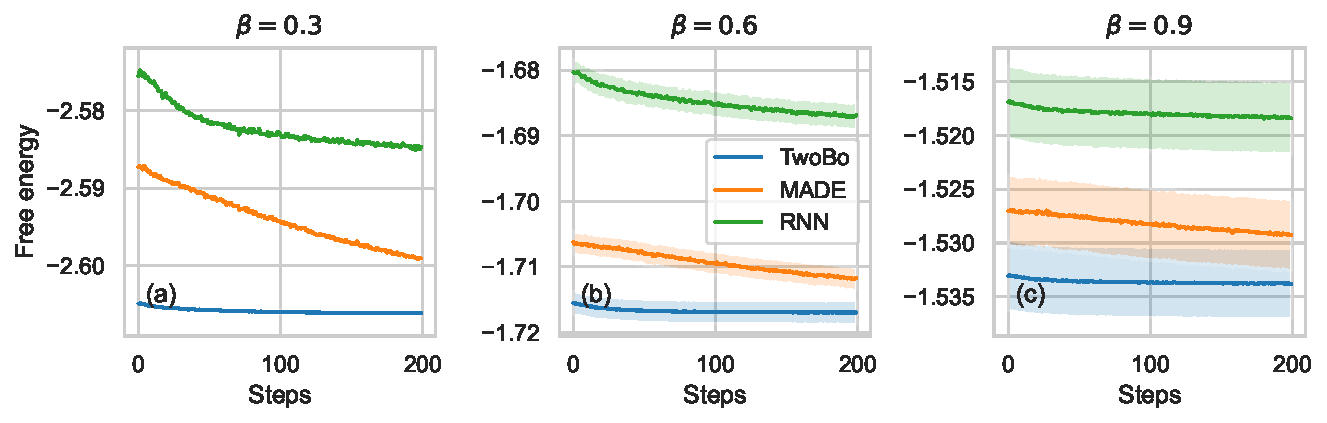
\includegraphics[width=\linewidth]{ch5/twobo_converge.pdf}
\caption[Convergence of TwoBo variational free energy in training]{
Convergence of variational free energy during the optimization steps in an annealing step, at different inverse temperatures $\beta$, on the 2D EA model with $N = 576$.
This figure is reproduced from Fig.~3 in Ref.~\cite{biazzo2024sparse}.
}
\label{fig:twobo-converge}
\end{figure}

\begin{figure}[htb]
\centering
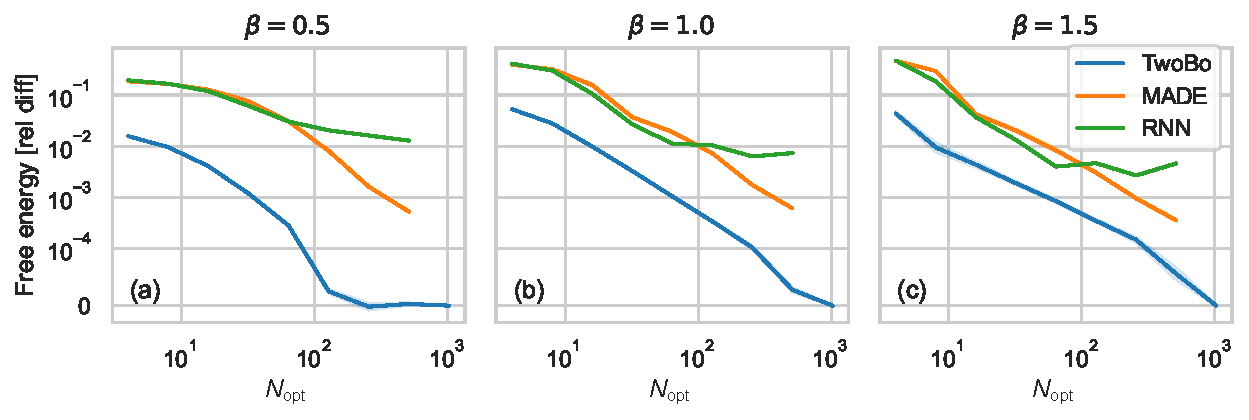
\includegraphics[width=\linewidth]{ch5/twobo_n_opt.pdf}
\caption[TwoBo variational free energy vs.\ annealing speed]{
Variational free energy as a function of the annealing speed, at different inverse temperatures $\beta$, on the 2D EA model with $N = 576$.
The annealing speed is controlled by the number of optimization steps $N_\text{opt} = 4, 8, 16, \ldots, 1024$ in each annealing step.
The variational free energy is shown as the relative difference from TwoBo at the same $\beta$ with $N_\text{opt} = 1024$.
The $y$-axis uses the logarithmic scale when the value is greater than $10^{-4}$.
This figure is reproduced from Fig.~4 in Ref.~\cite{biazzo2024sparse}.
}
\label{fig:twobo-n-opt}
\end{figure}

In addition to accuracy after training, TwoBo also has the advantage of fast convergence during training. As shown in \cref{fig:twobo-converge}, in each annealing step with a fixed $\beta$, TwoBo always starts from a lower variational energy and reaches convergence in fewer optimization steps. This advantage can be attributed to the incorporation of the interactions $\mJ$ in the parameters, which makes the initialization of the ansatz $q(\vs)$ physically feasible, i.e., closer to the target distribution $p_\text{B}(\vs)$ than a neural network with only random initialization.

This fast convergence also allows us to reduce the total computation time of the annealing procedure using a higher annealing speed. The annealing speed is controlled by the number of optimization steps $N_\text{opt}$ in each annealing step. As shown in \cref{fig:twobo-n-opt}, the variational free energy systematically decreases as $N_\text{opt}$ increases, presumably in a power law. In particular, TwoBo reaches the same variational free energy with almost an order of magnitude smaller $N_\text{opt}$ than MADE and RNN, which demonstrates its high efficiency in training. Therefore, we use only $N_\text{opt} = 200$ to achieve satisfactory results in \cref{fig:twobo-ea}, and each training can finish in an hour on a high-end GPU.

\subsubsection{Parameter efficiency}

\begin{figure}[htb]
\centering
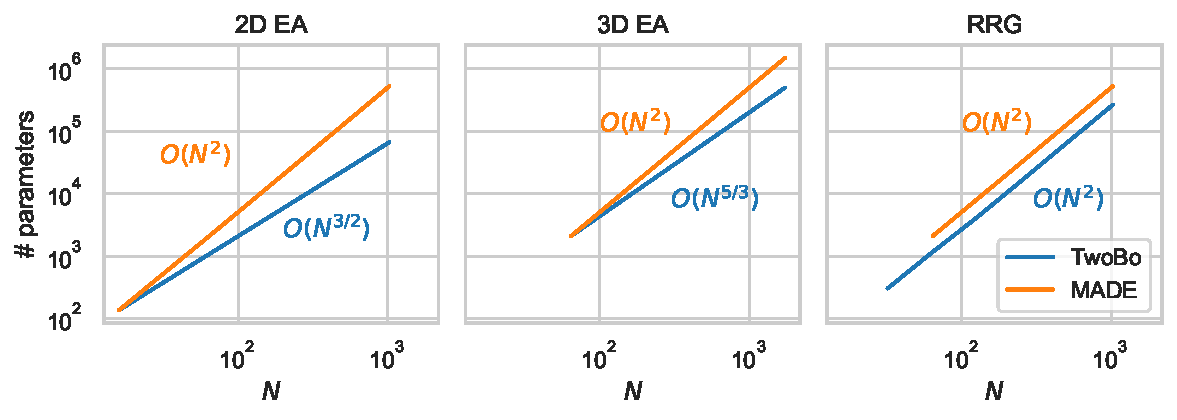
\includegraphics[width=\linewidth]{ch5/twobo_param.pdf}
\caption[Number of parameters vs.\ system size for TwoBo and MADE]{
Number of trainable parameters in TwoBo and MADE as a function of the system size $N$, on 2D grids, 3D grids, and RRGs.
This figure is reproduced from Fig.~S1 in the supplementary material for Ref.~\cite{biazzo2024sparse}.
}
\label{fig:twobo-param}
\end{figure}

\begin{figure}[htb]
\centering
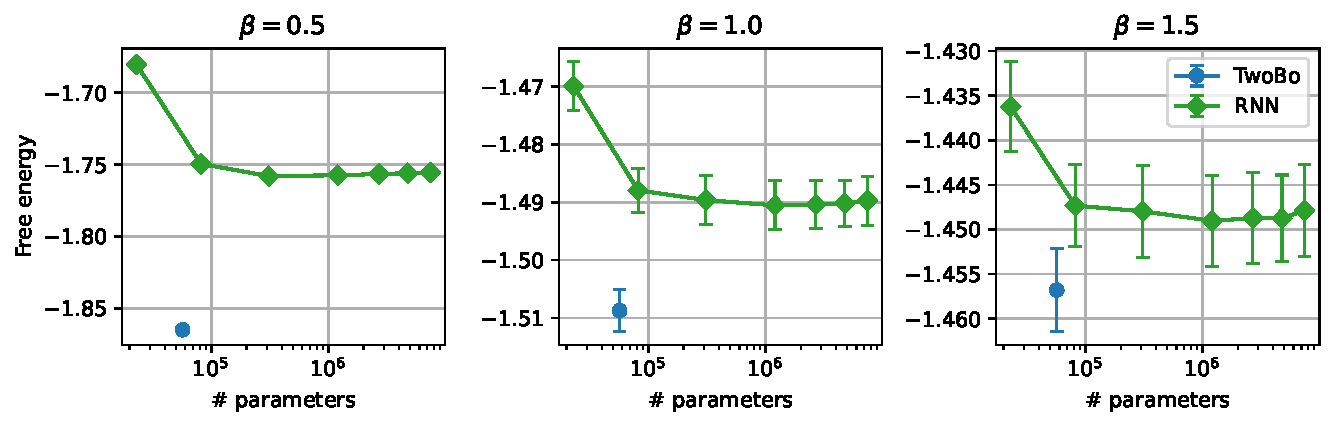
\includegraphics[width=\linewidth]{ch5/twobo_rnn_param.pdf}
\caption[Variational free energy vs.\ number of parameters for TwoBo and RNN]{
Variational free energy of TwoBo compared to RNN with different numbers of memory units ($2, 4, 8, 16, 24, 32, 40$), on the 2D EA model with $N = 576$.
This figure is reproduced from Fig.~S3 in the supplementary material for Ref.~\cite{biazzo2024sparse}.
}
\label{fig:twobo-rnn-param}
\end{figure}

Lastly, we investigate the empirical scaling of the number of trainable parameters in TwoBo with the system size. As shown in \cref{fig:twobo-param}, TwoBo has polynomially fewer parameters than MADE on 2D and 3D grids. However, for the RRGs without a local geometry, TwoBo no longer has polynomially fewer parameters, but only fewer by a constant coefficient of approximately $2$. These results are consistent with the theoretical analysis in \cref{sec:twobo-sparse}.

This advantage is more clearly demonstrated when we compare with RNN in the regime of numerous parameters. As shown in \cref{fig:twobo-rnn-param}, the TwoBo with few parameters gives a lower variational free energy than the RNN with a comparable number of parameters, and even if we enlarge the RNN by orders of magnitude, the variational free energy does not systematically decrease. These results emphasize the importance of the lightweight architecture with the physical knowledge in TwoBo, which can be more efficient than scaling up a general neural network architecture with increasing computation.

\subsection{Conclusion}

In conclusion, the TwoBo architecture incorporates the knowledge of the Boltzmann distribution and the sparse two-body interacting Hamiltonian into the neural network design, therefore achieves more accurate free energy estimation, faster training speed, and polynomially higher parameter efficiency compared to previous ARNN architectures. It opens a promising way to scale up the variational inference computation to larger systems and extract more physically interpretable results from neural networks.

\section{ARNN in importance sampling}
\label{sec:arnn-mcmc}

In the previous sections, we have seen the advantages of ARNN over previous ansatzes in variational inference. Meanwhile, as discussed in \cref{sec:compare-mcmc}, when unbiased estimations of observables rather than an upper bound of the free energy is desired, we can also use ARNN with the importance sampling in \cref{eq:importance-sampling} and the MCMC importance sampling in \cref{eq:mcmc-importance}.

Soon after Ref.~\cite{wu2019solving} introduced ARNN in statistical physics problems, Ref.~\cite{nicoli2020asymptotically} has proposed to use ARNN in the importance sampling and the MCMC importance sampling. However, Ref.~\cite{ciarella2023machine} has questioned the efficiency of these sampling methods on physical systems with complicated probability landscapes, such as the Potts model and the random graph coloring problem in the random first-order transition (RFOT) universality class. Moreover, Ref.~\cite{bialas2023analysis} has noticed that a reliable analysis of the autocorrelation time in \cref{eq:iat} is largely overlooked in the studies of these sampling methods, which is crucial to measuring the efficiency of MCMC methods. Fortunately, as discussed in \cref{sec:mode-collapse}, cluster update methods and symmetry operations can help to overcome the problem of mode collapse in first-order phase transitions, while reducing the autocorrelation time as well.

In the following, we present a sampling method proposed in Ref.~\cite{wu2021unbiased}, which constructs cluster updates using the AR property of the ansatz, and applies the symmetries of the physical system, to achieve the unbiased sampling with high efficiency even if the physical system exhibits a first-order phase transition.

\subsection{Neural cluster updates with symmetries (NCUS)}
\label{sec:ncus}

\begin{algorithm}[H]
\caption[Neural cluster updates with symmetries (NCUS)]{
A sampling step in NCUS for a system of $N$ spins on a square lattice with translation, $D_4$ lattice reflection, and $\bbZ_2$ spin flipping symmetries.
}
\label{alg:ncus}
\begin{algorithmic}[1]
\STATE Input the current configuration $\vs$
\STATE Sample an integer $k \in \{1, \ldots, N\}$ from the distribution $P_\text{cluster}(k)$
\STATE Sample the last $k$ spins and propose the configuration $\vs'$
\STATE Accept $\vs \gets \vs'$ with the probability in \cref{eq:ncus-a}
\STATE Translate $\vs$ by a random displacement
\STATE Reflect $\vs$ along the $x$-axis, the $y$-axis, and the diagonal, each with $50\%$ probability
\STATE Reflect $\vs$ along the $z$-axis (flip all spins) with $50\%$ probability
\STATE Output $\vs$ as a sample in the Markov chain
\end{algorithmic}
\end{algorithm}

\begin{figure}[htb]
\centering
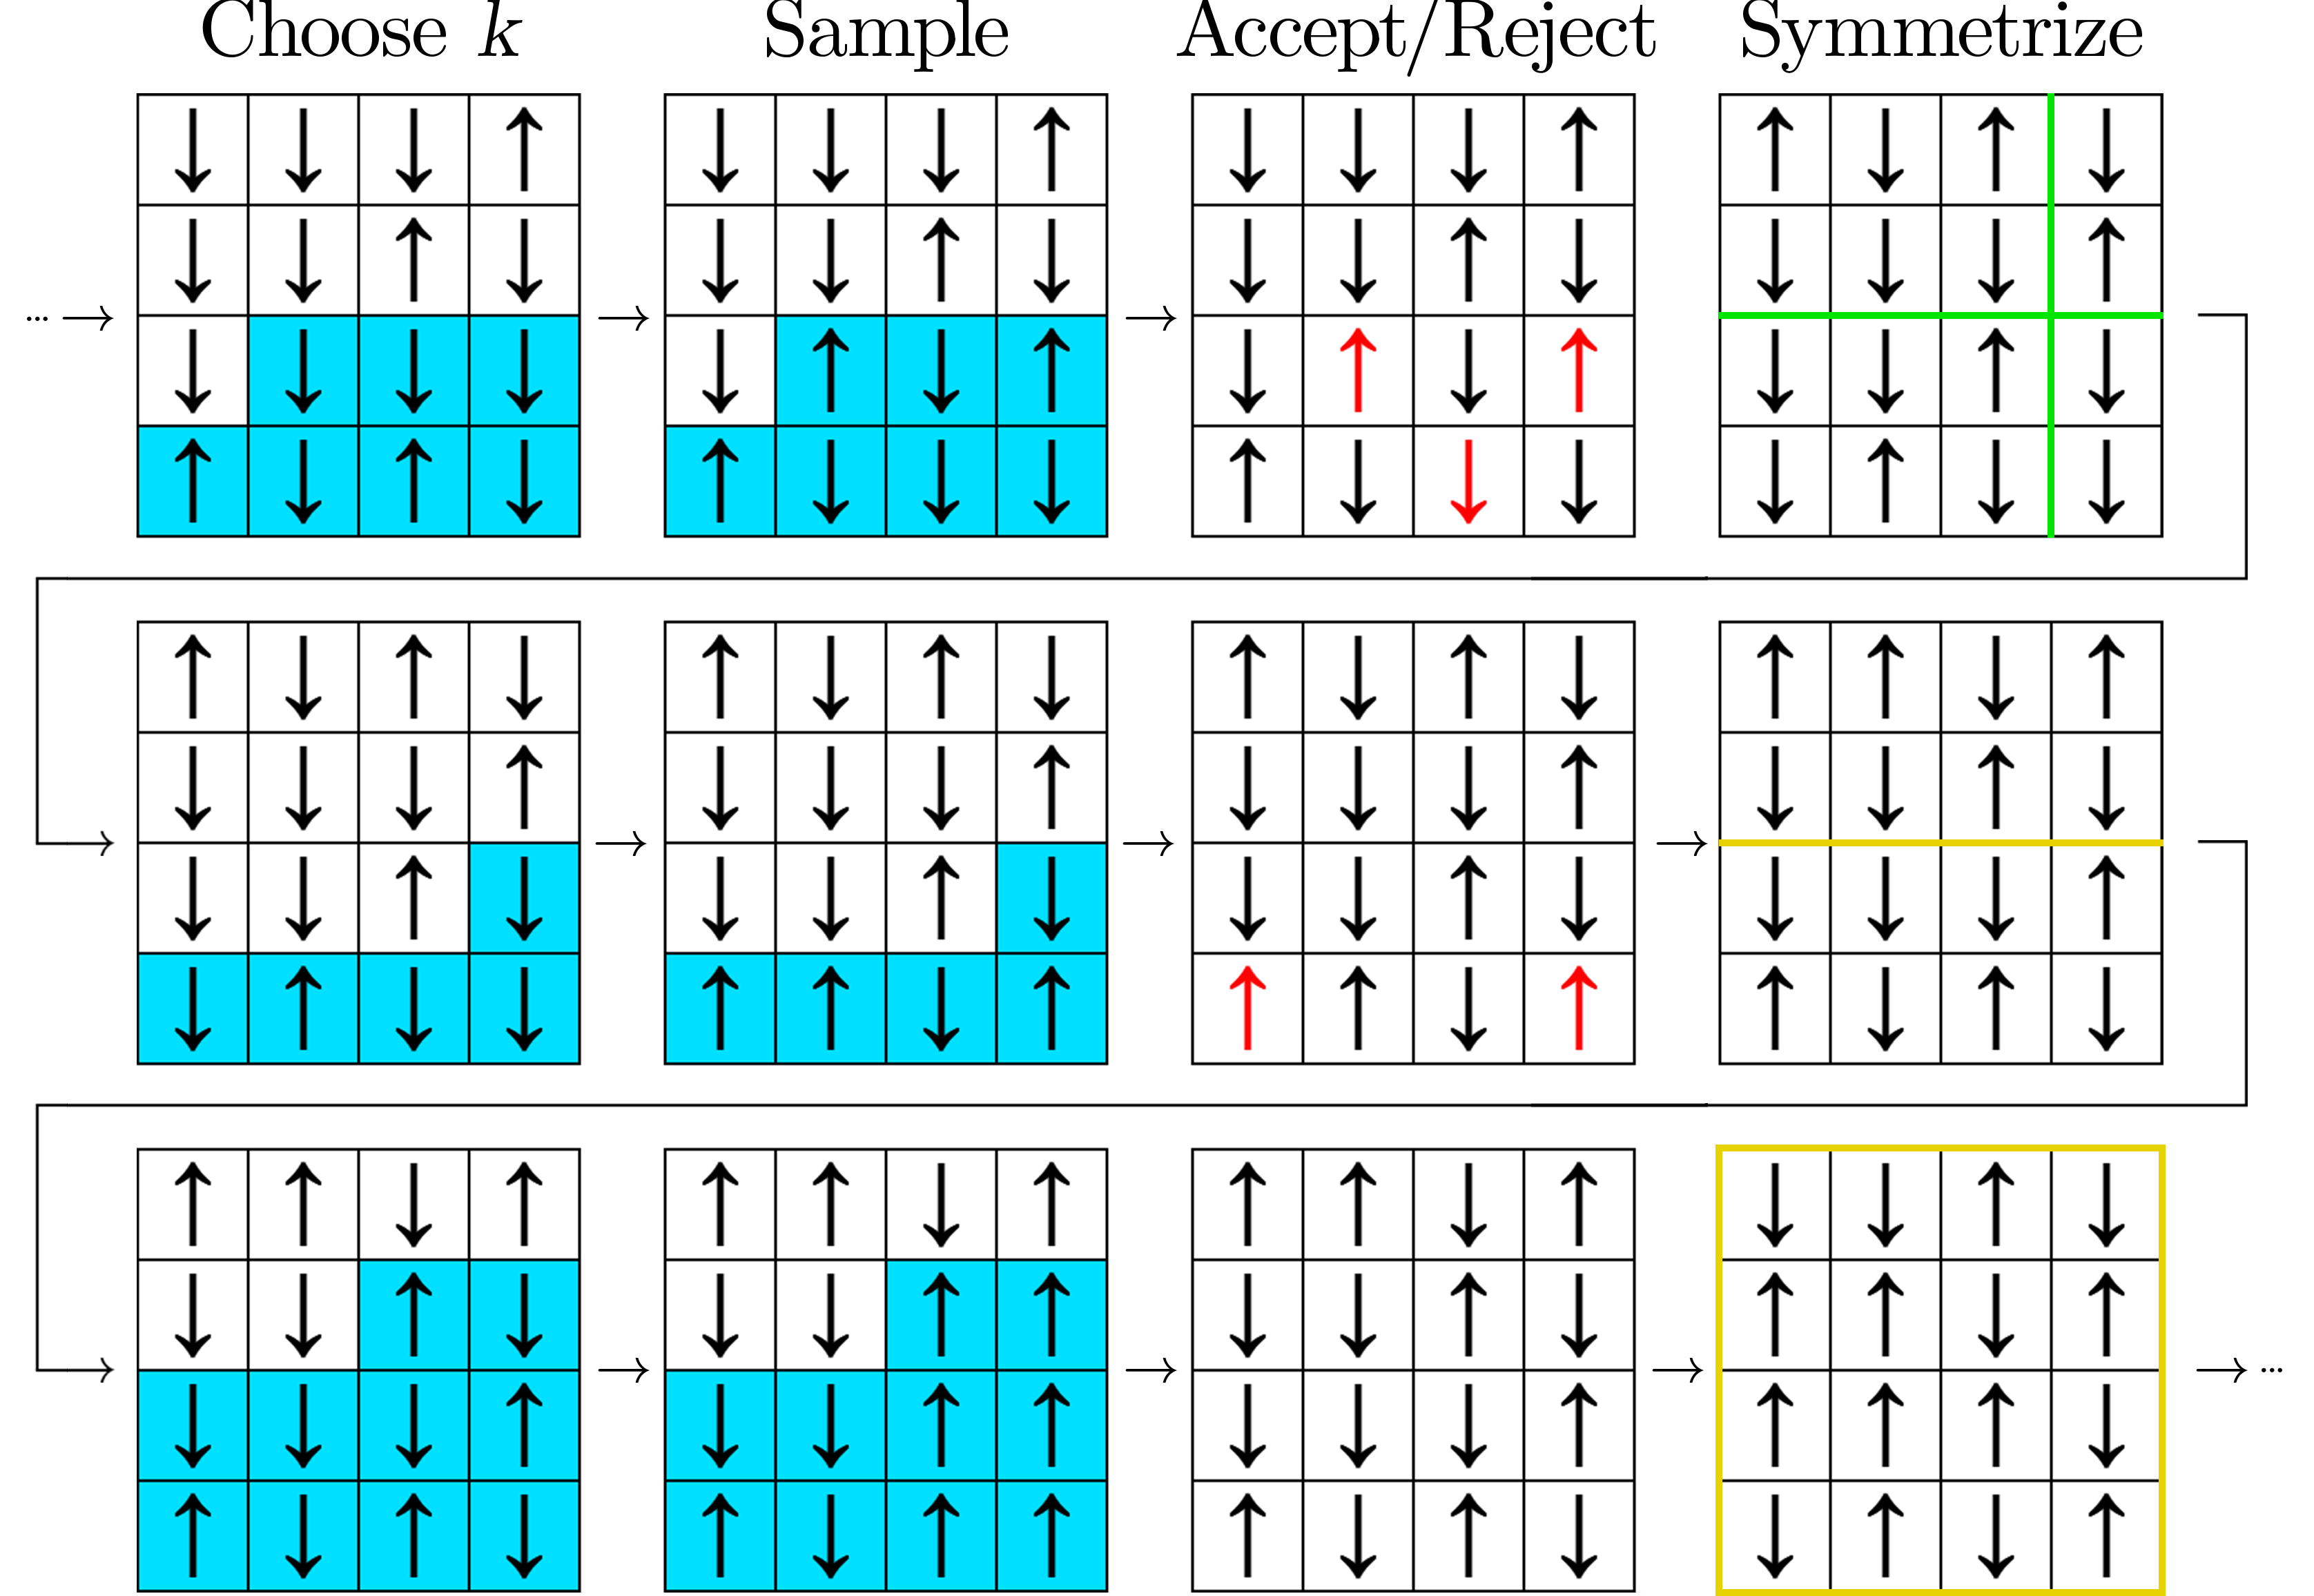
\includegraphics[width=0.6\linewidth]{ch5/ncus_proc.png}
\caption[Procedure of neural cluster updates with symmetries (NCUS)]{
Examples of three steps of NCUS applied to a system on the $4 \times 4$ square lattice. The operations in several lines of \cref{alg:ncus} are visualized by colors.
In line $2$, the last $k$ spins chosen are highlighted in {\color[HTML]{1f77b4} blue}.
In line $3$, some of them are flipped in the proposal.
Then in line $4$, if the proposal is actually accepted, the flipped spins are shown in {\color[HTML]{d62728} red}.
In line $5$, the original borders of the lattice before the translation are shown in {\color[HTML]{2ca02c} green}.
In line $6$, the plane of reflection is shown in {\color[HTML]{bcbd22} yellow}, and a reflection along the $z$-axis (across the $x y$-plane) is indicated by yellow borders around the lattice.
This figure is reproduced from Fig.~1 in Ref.~\cite{wu2021unbiased}.
}
\label{fig:ncus-proc}
\end{figure}

During the MCMC importance sampling procedure in \cref{eq:mcmc-importance}, we propose new configurations $\vs'$ from the ansatz $q(\vs)$. When the ansatz is factorized into the AR conditional distributions in \cref{eq:autoreg}, we notice that it is possible to avoid generating all $N$ spins from the beginning, but only the last $k$ spins. In this way, the acceptance in \cref{eq:mcmc-importance} becomes
\begin{equation}
A(\vs \to \vs') = \min\left( 1, \frac{p(\vs')}{p(\vs)} \prod_{i = N - k + 1}^N \frac{q_i(s_i \mid \vs_{< i})}{q_i(s'_i \mid \vs'_{< i})} \right),
\label{eq:ncus-a}
\end{equation}
which is usually close to $1$ when $k$ is small. With suitable values of $k$, we can enjoy the efficiency of cluster updates, which overcome both the inability of local updates to transition through energy barriers and the low acceptance probability of global updates. We refer to the distribution of $k$ as $P_\text{cluster}(k)$, and it can be the uniform distribution over $\{1, \ldots, N\}$ without loss of generality. Comparisons between the choices of $P_\text{cluster}(k)$ will be presented in \cref{fig:ncus-pk}.

The construction of the above clusters introduces an obvious bias that the spins closer to the end of the autoregressive order will be more frequently flipped. To flip every spin with the same frequency on average, we randomly apply the symmetry operations of the Hamiltonian to the samples in the Markov chain. These operations act as global updates that transition through local energy barriers, and they are never rejected because they conserve the energy and thus have an acceptance probability of $1$. Combining the cluster updates and the symmetry operations, we refer to the resulting algorithm as neural cluster updates with symmetries (NCUS). This algorithm is described in \cref{alg:ncus} and visualized in \cref{fig:ncus-proc}.

\subsection{Numerical results}

\subsubsection{Ising model}

\begin{figure}[htb]
\centering
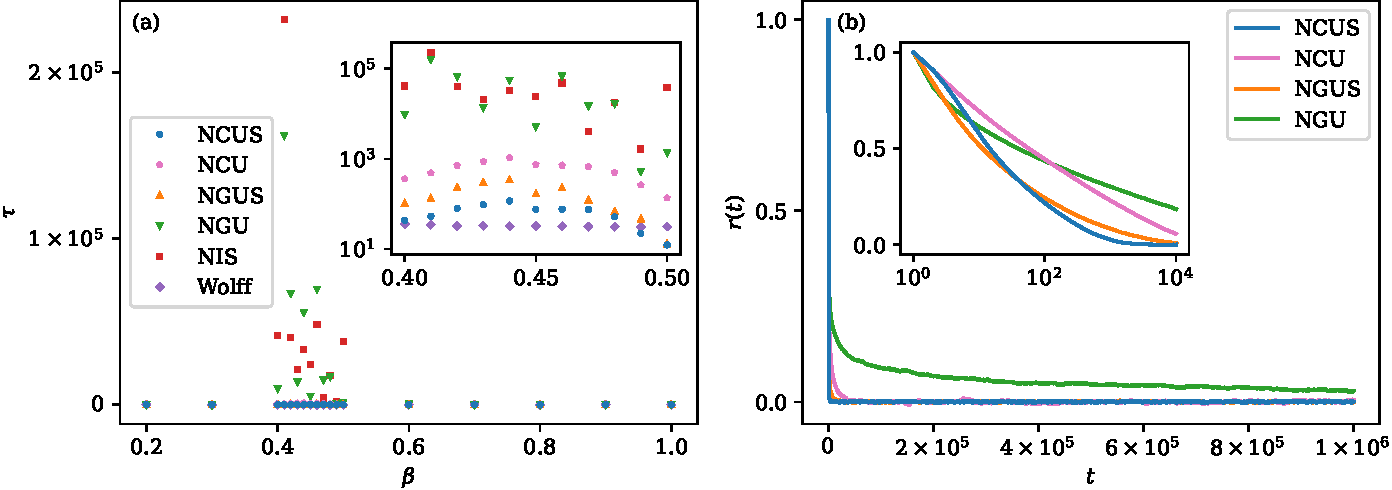
\includegraphics[width=\linewidth]{ch5/ncus_ising_autocorr.pdf}
\caption[NCUS results of Ising model]{
(a) Autocorrelation time $\tau$ for the Ising model on the $16 \times 16$ square lattice, at varying inverse temperature $\beta$, given by the sampling methods presented in this section.
The inset focuses on their behaviors around the critical point and uses the logarithmic scale on the $y$-axis. \\
(b) Normalized autocorrelation $r(t)$ at $\beta = 0.44$ around the critical point.
The inset uses the logarithmic scale on the $x$-axis to focus on their behaviors at small $t$.
This figure is reproduced from Fig.~2 in Ref.~\cite{wu2021unbiased}.
}
\label{fig:ncus-ising-autocorr}
\end{figure}

To demonstrate the performance of NCUS, we first conduct numerical experiments using the Ising model on the square lattice with PBC, which has translation, $D_4$ lattice reflection, and $\bbZ_2$ spin flipping symmetries. We compare NCUS with \cref{eq:importance-sampling}, referred to as neural importance sampling (NIS) here, as well as \cref{eq:mcmc-importance}, referred to as neural global updates (NGU) here. As ablation studies, we also consider neural global updates with symmetries (NGUS) and neural cluster updates (NCU) without symmetries. In addition, the well-established Wolff cluster update algorithm~\cite{wolff1989collective} is taken for comparison.

In all the neural sampling methods, we use a same neural network trained using the usual variational method. The network is a convolutional ARNN with approximately $4 \times 10^3$ parameters, which is much smaller compared to the networks used in \cref{sec:made}, as we now emphasize efficient sampling and correction to the non-ideally trained ansatz $q(\vs)$. After the sampling, the mean free energies given by all the methods are apparently close to each other, so we focus on analyzing the autocorrelation times of the free energy as defined in \cref{eq:iat}, which determine the error bars. For NIS, although it does not produce a Markov chain, we still use the effective sample size in \cref{eq:eff-sample-size,eq:eff-sample-size-w} to define an effective autocorrelation time for comparison.

As shown in \cref{fig:ncus-ising-autocorr}~(a), around the critical point, NCUS produces autocorrelation times lower by orders of magnitude than the previous neural sampling methods, while the autocorrelation times of NGU and NIS are pathologically high. A closer look at the normalized autocorrelation functions in \cref{fig:ncus-ising-autocorr}~(b) confirms these results, where the samples from NCUS quickly decorrelate in less than $10^3$ steps, while those from NGU cannot decorrelate after as many as $10^5$ steps. Moreover, the autocorrelation times of NCUS are comparable to those of the Wolff algorithm, although the latter is specifically designed for the Ising model. These results illustrate the advantage of cluster updates and symmetry operations in alleviating the problem of critical slowing down, as discussed in \cref{sec:critical-slow}.

\subsubsection{Frustrated plaquette model (FPM)}
\label{sec:ncus-fpm}

\begin{figure}[htb]
\centering
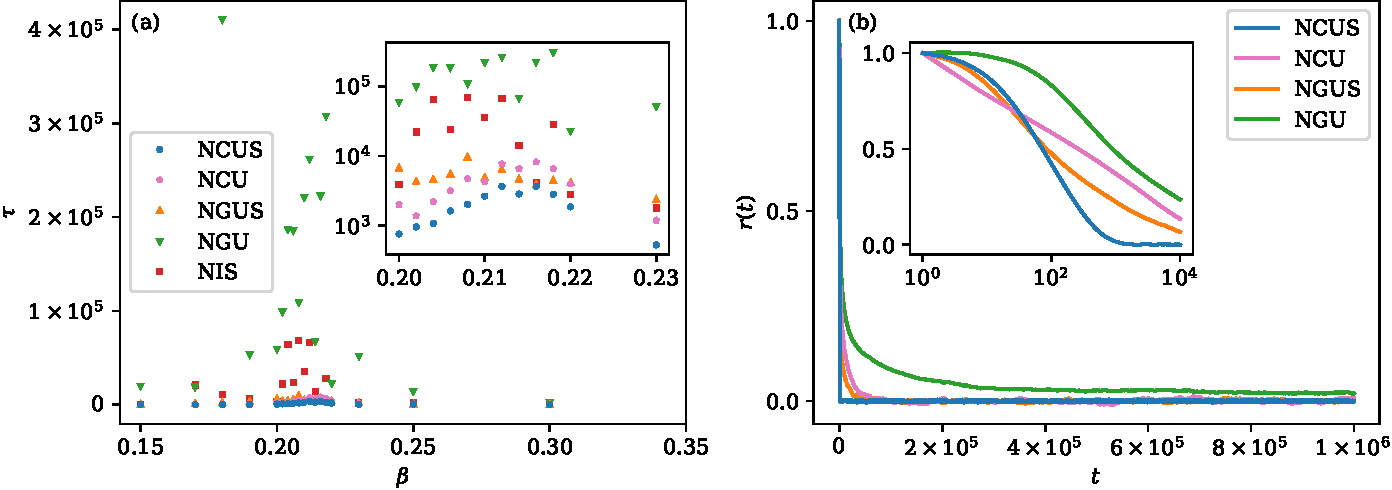
\includegraphics[width=\linewidth]{ch5/ncus_fpm_autocorr.pdf}
\caption[NCUS results of FPM]{
(a) Autocorrelation time $\tau$ for the FPM on the $32 \times 32$ square lattice, at varying inverse temperature $\beta$, given by the sampling methods in this section.
The inset focuses on their behaviors around the critical point and uses the logarithmic scale on the $y$-axis. \\
(b) Normalized autocorrelation $r(t)$ at $\beta = 0.2$ around the critical point.
The inset uses the logarithmic scale on the $x$-axis to focus on their behaviors at small $t$.
This figure is reproduced from Fig.~4 in Ref.~\cite{wu2021unbiased}.
}
\label{fig:ncus-fpm-autocorr}
\end{figure}

Next, we apply the sampling methods to the frustrated plaquette model (FPM) discussed in \cref{sec:fpm}, which is more difficult than the Ising model due to the first-order phase transition induced by the frustrated $J_3$ interactions and the plaquette interactions. Moreover, we increase the system size from $16 \times 16$ to $32 \times 32$. This time, the Wolff algorithm is no longer applicable as it is designed only for systems with two-body interactions. In contrast, the neural sampling methods are general enough to handle the plaquette interactions.

As shown in \cref{fig:ncus-fpm-autocorr}, the results have a trend similar to those for the Ising model around the critical point. The autocorrelation times of NCUS can be as high as $O(10^3)$, but it is still practical to obtain reliable estimations of the free energy with the error bars derived from them, and they are lower by orders of magnitude than the results from the previous neural sampling methods. These results provide evidence that cluster updates and symmetry operations help to alleviate the problem of mode collapse with the presence of first-order phase transitions aforementioned in \cref{sec:mode-collapse}.

\subsubsection{Choices of the distribution $P_\text{cluster}(k)$}

\begin{figure}[htb]
\centering
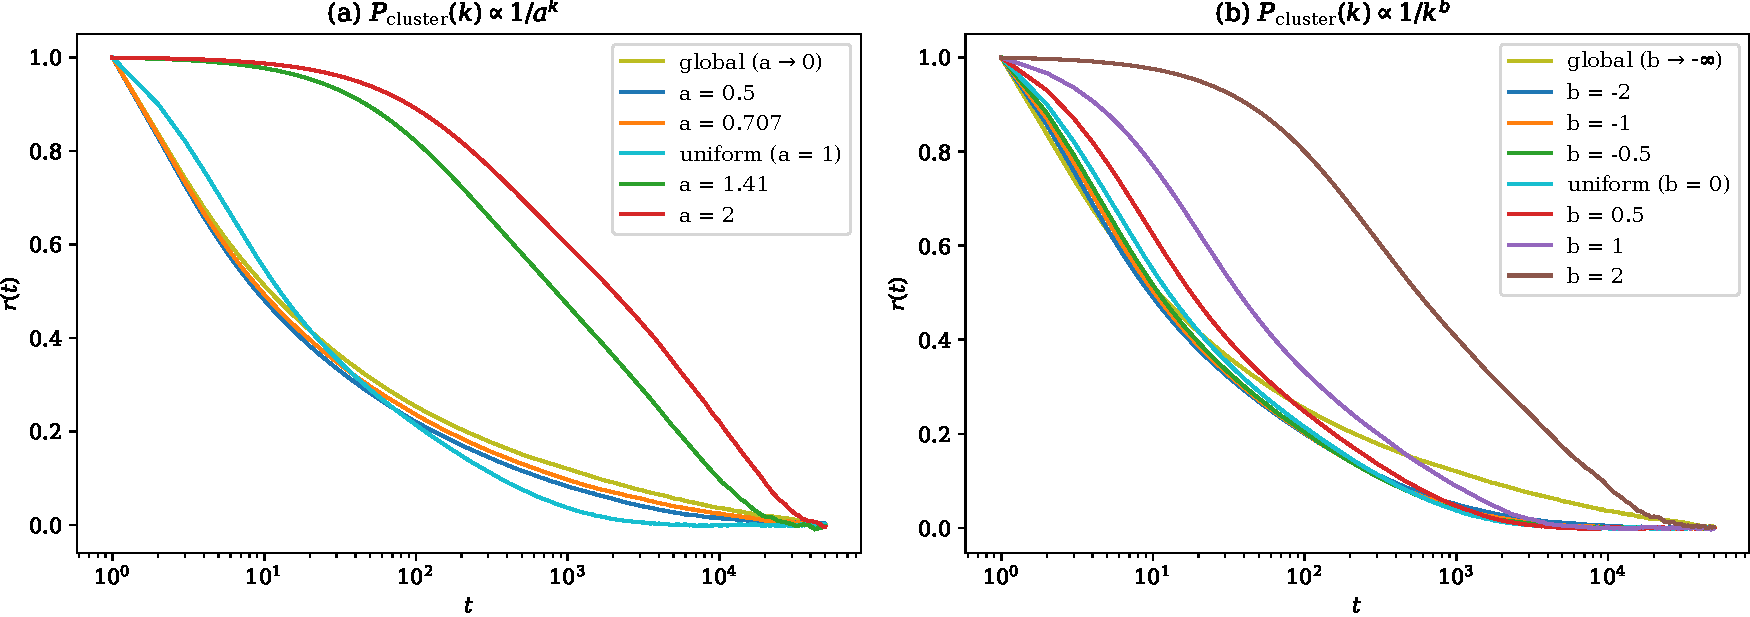
\includegraphics[width=\linewidth]{ch5/ncus_pk.pdf}
\caption[Choices of the distribution $P_\text{cluster}(k)$ in NCUS]{
Normalized autocorrelation $r(t)$ given by NCUS on the $16 \times 16$ Ising model at inverse temperature $\beta = 0.44$, with different choices of $P_\text{cluster}(k)$ from exponential and power distributions.
This figure is reproduced from Fig.~S1 in the supplemental material for Ref.~\cite{wu2021unbiased}.
}
\label{fig:ncus-pk}
\end{figure}

The efficiency of NCUS can depend on the distribution $P_\text{cluster}(k)$ of the number of spins to generate. In the above results, we have arbitrarily chosen the uniform distribution. Empirical comparisons between different choices of exponential distributions $P_\text{cluster}(k) \propto 1 / a^k$ and power distributions $P_\text{cluster}(k) \propto 1 / k^b$, where $a$ and $b$ are adjustable parameters, are shown in \cref{fig:ncus-pk}, respectively. The uniform distribution gives an autocorrelation time comparable or lower to all other distributions we have tested. Moreover, it also outperforms the more naive method of always using the same number, i.e., $P_\text{cluster}(k) = \delta(k - k')$ for all $k' \in \{1, \ldots, N\}$. It remains an open question to reveal the relation between the optimal $P_\text{cluster}(k)$ and the properties of the target distribution $p(\vs)$ as well as the ansatz $q(\vs)$, using theoretical analysis on the Markov chain transitions.

\subsection{Conclusion}

In conclusion, the NCUS algorithm utilizes the cluster updates constructed by the AR property of the ansatz, as well as the symmetries of the physical system, to produce substantially lower autocorrelation times than the conventional global update method around the critical point, and more reliable estimations of observables with lower error bars in consequence.

We look forward to more research combining the strengths of the techniques presented in this section, including neural networks as highly expressive heuristics for complicated multivariate distributions, autoregressive models with exact sampling and normalized probability evaluation, physical properties such as symmetries and sparsity incorporated into network architectures, and cluster updates that alleviate the problems of critical slowing down and mode collapse, which will eventually lead to solutions for physical systems with unprecedented size and complexity.

\part{Computational techniques for quantum systems}
\chapter{Unbiased evaluation of ground state}

The previous part have let us seen exact sampling methods, particularly autoregressive neural networks (ARNN), achieve higher accuracy and efficiency in approximating classical many-body systems. Now we move on to investigate quantum systems, which are known to be more intricate than their classical counterparts. Even though we only focus on their ground states, rather than finite-temperature ensembles or dynamics, they involve peculiar issues that do not exist in the classical world, such as vanishing energy gaps, sign structures, and entanglements.

In this part, we first review the traditional methods of exact diagonalization (ED), path integral Monte Carlo (PIMC), variational Monte Carlo (VMC), and tensor networks. They not only share some common issues with Markov chain Monte Carlo (MCMC) and variational methods discussed in the previous part, but are also affected by the peculiar issues in quantum systems. Then we introduce a variational ansatz named tensor-RNN, which combines the strengths of tensor networks and recurrent neural networks (RNN) to shed new light on both the analytical and the numerical aspects of quantum systems. Moreover, we discuss the results from VarBench, an extensive project to benchmark the performances of variational methods on quantum many-body systems, which witnesses the recent development in the field, including exact sampling methods. Lastly, we present NetKet, a software package that we have developed to ease the implementation of all the computational techniques aforementioned, with attention on the integration of exact sampling in it.

\section{Imaginary time evolution (ITE)}
\label{sec:ite}

The ground state vector $\ket{\psi_0}$ provides the most complete information of a quantum many-body system at ground state, which allows obtaining all its properties. We start from a straightforward analytical method to evaluate $\ket{\psi_0}$, using the basic properties of eigenstates. We apply the exponential of the system's Hamiltonian $\hat{H}$, with a scaling parameter $\tau$, on an arbitrary initial state $\ket{\psiinit}$, and obtain
\begin{equation}
\ket{\psi_\tau} = \rme^{-\tau \hat{H}} \ket{\psiinit},
\label{eq:ite-psi-tau}
\end{equation}
where we temporarily ignore the normalization of the states. Because of the orthogonality and the completeness of the eigenstates, the initial state can be decomposed into a linear combination of them:
\begin{equation}
\ket{\psiinit} = \sum_i c_i \ket{\psi_i},
\end{equation}
where $\ket{\psi_i}$ is the $i$-th lowest eigenstate, and $c_i$ is the corresponding coefficient that can be determined by projection. Under the action of the Hamiltonian, each eigenstate is scaled by its energy $E_i$:
\begin{equation}
\hat{H} \ket{\psi_i} = E_i \ket{\psi_i}.
\end{equation}
The exponential of an operator is defined by the Taylor expansion:
\begin{equation}
\rme^{-\tau \hat{H}} = \sum_{j = 0}^\infty \frac{1}{j!} (-\tau \hat{H})^j,
\label{eq:ite-taylor}
\end{equation}
assuming it converges. Therefore, \cref{eq:ite-psi-tau} becomes
\begin{equation}
\ket{\psi_\tau} = \sum_i c_i \rme^{-\tau E_i} \ket{\psi_i}.
\end{equation}
In the limit $\tau \to \infty$, as the exponential $\rme^{-\tau E_0}$ grows faster than all other terms, the resulting state $\ket{\psi_\tau}$ is dominated by the ground state $\ket{\psi_0}$. This is true regardless of the coefficients $c_i$, as long as $c_0 \neq 0$, i.e., the initial state is not orthogonal to the ground state, which is usually fulfilled if the initial state is randomly chosen. In the case of degenerate ground states, this method produces an arbitrary one among them, depending on the choice of the initial state.

Recovering the normalization, we have
\begin{equation}
\ket{\psi_0} = \lim_{\tau \to \infty} \frac{\ket{\psi_\tau}}{\sqrt{\ip{\psi_\tau}}}.
\label{eq:ite}
\end{equation}
This method is known as the imaginary time evolution (ITE)~\cite{goldberg1967integration}, because it has a similar form to the conventional notation of time evolution under the Schrödinger equation:
\begin{equation}
\ket{\psi(t)} = \rme^{-\rmi \hat{H} t} \ket{\psiinit},
\end{equation}
which becomes \cref{eq:ite-psi-tau} if we let the time be an imaginary number $t = -\rmi \tau$.

The asymptotic convergence speed of the limit in \cref{eq:ite} depends on the energy gap $\Delta E = E_1 - E_0$ between the ground state $\ket{\psi_0}$ and the first excited state $\ket{\psi_1}$, as we can see from the ratio of their overlaps with $\ket{\psi_\tau}$:
\begin{equation}
\frac{\ip{\psi_1}{\psi_\tau}}{\ip{\psi_0}{\psi_\tau}} \propto \rme^{-\tau \Delta E}. \label{eq:ite-converge}
\end{equation}
This is a root cause of various numerical difficulties in gapless systems, including systems in disordered or critical regimes, such as spin liquids.

\section{Exact diagonalization (ED)}
\label{sec:ed}

When numerically implementing ITE, we discretize the limit $\tau \to \infty$ into an iterative scheme, and do the normalization in each iteration to ensure numerical stability:
\begin{align}
\ket{\psi'_k} &= \rme^{-\Delta \tau \hat{H}} \ket{\psi_k}, \\
\ket{\psi_{k + 1}} &= \frac{\ket{\psi'_k}}{\sqrt{\ip{\psi'_k}}}.
\end{align}
Meanwhile, we can only keep the first order in the Taylor expansion of $\rme^{-\Delta \tau \hat{H}}$, therefore \cref{eq:ite-taylor} becomes
\begin{equation}
\rme^{-\Delta \tau \hat{H}} \approx 1 - \Delta \tau \hat{H}.
\end{equation}
Given that the time step $\Delta \tau$ is small enough and the number of iterations $k$ is large enough, $\ket{\psi_k}$ converges to the desired $\ket{\psi_0}$. This method is known as the power iteration~\cite{mises1929praktische}. It falls in a broader family of iterative methods to compute the lowest one or few eigenvalues and eigenvectors of a matrix, where the Lanczos algorithm~\cite{lanczos1950iteration} is particularly well-known, following various algorithmic improvements and software implementations~\cite{knyazev2001toward, stathopoulos2010primme}. The convergence speeds of those algorithms also depend on the energy gap $\Delta E$, as shown in \cref{eq:ite-converge}.

In the context of quantum physics, this kind of methods are referred to as the exact diagonalization (ED)~\cite{weisse2008exact}, because they do not involve any approximation or stochastic estimation in the obtained states. However, we can only perform ED on small systems, because the storage of the entire state vector and the multiplication with the Hamiltonian become impractical on larger systems due to the exponentially high dimension of the Hilbert space aforementioned in \cref{sec:qu-sys}. As of this writing, the largest ED computation has been performed on $50$ spin-$1/2$ particles~\cite{wietek2018sublattice}, which utilizes the symmetries of the physical system to reduce the dimension of the Hilbert space, as well as implementing sophisticated parallelization and storage strategies on the supercomputer. Despite its exponential computational complexity, ED is still a necessary method to provide initial insights at small system sizes when investigating an unfamiliar quantum model, and it serves as the ground truth to test the correctness of more advanced computational techniques.

\section{Quantum Monte Carlo (QMC)}
\label{sec:qmc}

On larger systems where the exact evaluation of the ground state is impractical, we can use stochastic methods to approximate it, which fit into the framework of Monte Carlo estimation aforementioned in \cref{sec:monte-carlo}. Quantum Monte Carlo (QMC) has become a gross term referring to these methods.

In the following, we present a QMC scheme directly following the above derivation of ITE. Temporarily ignoring the normalization, we discretize each component of the ground state vector $\ip{\vs}{\psi_0}$ with
\begin{align}
\ip{\vs}{\psi_0} &= \lim_{\tau \to \infty} \mel{\vs}{\rme^{-\tau \hat{H}}}{\psiinit} \\
&= \lim_{N_\tau \to \infty} \mel{\vs}{\edthp^{N_\tau}}{\psiinit} \\
&= \lim_{N_\tau \to \infty} \sum_{\vs_1, \ldots, \vs_{N_\tau}}\!\!\!\!\mel{\vs}{\edth}{\vs_1} \mel{\vs_1}{\edth}{\vs_2} \cdots \mel{\vs_{N_\tau - 1}}{\edth}{\vs_{N_\tau}} \ip{\vs_{N_\tau}}{\psiinit},
\end{align}
where the auxiliary configurations $\vs_1, \ldots, \vs_{N_\tau}$ are inserted using the completeness of basis states. They are used to define the short-time propagator
\begin{equation}
G(\vs, \vs') = \mel{\vs}{\edth}{\vs'}.
\end{equation}
As long as $\Delta \tau$ is small, $G(\vs, \vs')$ can be computed with high accuracy, where the Trotter--Suzuki decomposition~\cite{suzuki1976generalized} is usually applied.

Using this discretization to estimate the energy, and recovering the normalization, we have
\begin{align}
E &= \lim_{\tau \to \infty} \frac{\ev{\rme^{-\tau \hat{H}} \hat{H}\,\rme^{-\tau \hat{H}}}{\psiinit}}{\ev{\rme^{-\tau \hat{H}} \rme^{-\tau \hat{H}}}{\psiinit}} \\
&= \lim_{\tau \to \infty} \frac
{\ev{\rme^{-2 \tau \hat{H}} \hat{H}}{\psiinit}}
{\ev{\rme^{-2 \tau \hat{H}}}{\psiinit}} \label{eq:pimc-commute} \\
&= \lim_{\tau \to \infty} \frac
{\sum_{\vs, \vs'} \mel{\psiinit}{\rme^{-2 \tau \hat{H}}}{\vs} \mel{\vs}{\hat{H}}{\vs'} \ip{\vs'}{\psiinit}}
{\ev{\rme^{-2 \tau \hat{H}}}{\psiinit}} \\
&= \lim_{\tau \to \infty} \frac
{\sum_\vs \mel{\psiinit}{\rme^{-2 \tau \hat{H}}}{\vs} \ip{\vs}{\psiinit} \sum_{\vs'} \mel{\vs}{\hat{H}}{\vs'} \frac{\ip{\vs'}{\psiinit}}{\ip{\vs}{\psiinit}}}
{\ev{\rme^{-2 \tau \hat{H}}}{\psiinit}} \\
&= \lim_{N_\tau \to \infty} \sum_\svs \varPi(\svs) E_\text{loc}(\vs_{N_\tau}), \label{eq:pimc}
\end{align}
where $\svs = (\vs_0, \vs_1, \ldots, \vs_{N_\tau})$ denotes all the auxiliary configurations, also known as the integration path, and
\begin{align}
\varPi(\svs) &= \frac{\tilde{\varPi}(\svs)}{\sum_\svs' \tilde{\varPi}(\svs')}, \\
\tilde{\varPi}(\svs) &= \psiinit^*(\vs_0) G(\vs_0, \vs_1) G(\vs_1, \vs_2) \cdots G(\vs_{N_\tau - 1}, \vs_{N_\tau}) \psiinit(\vs_{N_\tau}), \label{eq:pimc-pi} \\
E_\text{loc}(\vs) &= \sum_{\vs'} H(\vs, \vs') \frac{\psiinit(\vs')}{\psiinit(\vs)}.
\end{align}

The resulting \cref{eq:pimc} has a similar form to the weighted summation in \cref{eq:cl-obs}. If the weight $\varPi(\svs) \ge 0$ for all $\svs$, we can interpret it as a probability distribution, and estimate \cref{eq:pimc} using the Monte Carlo summation in \cref{eq:monte-carlo}. This method requires samples of $\svs$ generated from $\varPi(\svs) \ge 0$, and each sample contains $N (N_\tau + 1)$ scalar variables, where $N$ is the system size. This is an unbiased estimator of $E$ only when $N_\tau \to \infty$, and in practice we usually need a large $N_\tau$ such that $N_\tau \Delta \tau \gg 1$, which leads to much higher computational cost than Monte Carlo methods for the corresponding classical system. The evaluation of \cref{eq:pimc-pi} not only requires  accurately and efficiently computing the propagator $G(\vs, \vs')$, but also the initial wave function $\psi(\vs)$, and a good choice of $\ket{\psi}$ that is close to the ground state can significantly reduce the magnitude of $N_\tau$ needed. In addition, we note that \cref{eq:pimc-commute} holds not only when estimating the energy, but also any observable that commutes with $\hat{H}$.

This method is commonly referred to as the path integral Monte Carlo (PIMC)~\cite{barker1979quantum, raedt1985monte}, and a particular method to sample $\svs$ is known as the reptation Monte Carlo~\cite{baroni1999reptation}. For some physical systems, this kind of QMC computations have successfully achieved numerically exact results~\cite{todo2001cluster}, which can serve as the ground truth to test the correctness of other methods even if the ED result is unavailable.

\section{Sign problem}

The above discussion reveals a peculiar caveat in quantum systems: The distribution of a classical ensemble always has $p(\vs) \ge 0$, but the weight in \cref{eq:pimc} may not satisfy $\varPi(\svs) \ge 0$, and the Monte Carlo estimator is invalid in this case, which is known as the sign problem~\cite{loh1990sign, troyer2005computational}. In spin systems, the sign problem is usually a result of the frustrated interactions between the particles~\cite{henelius2000sign}. It is even more prevalent in fermionic systems, where the wave function frequently changes its sign because of the anti-commutation of the particles.

A quick remedy is to factor out the sign from the weight:
\begin{align}
E &= \lim_{N_\tau \to \infty} \sum_\svs \varPi'(\svs) E'_\text{loc}(\svs), \label{eq:pimc-sign} \\
\varPi'(\svs) &= \frac{|\tilde{\varPi}(\svs)|}{\sum_\svs' |\tilde{\varPi}(\svs')|}, \\
E'_\text{loc}(\svs) &= \sign\left( \tilde{\varPi}(\svs) \right) E_\text{loc}(\vs_{N_\tau}). \label{eq:pimc-eloc-sign}
\end{align}
However, the intrinsic complexity of the wave function does not simply disappear. Unlike the classical local free energy $F_\text{loc}(\vs)$ in \cref{eq:fq-loc}, which is usually far below zero when $s$ is around the ground state, the local energy $E'_\text{loc}(\svs)$ in \cref{eq:pimc-eloc-sign} can frequently change its sign as the integration path $\svs$ changes. In \cref{eq:pimc-sign}, there can be many positive and negative terms cancelling out, which lead to a small mean value and a large variance of the estimator, and prevents the result from achieving high accuracy with reliable error estimation.

As a well-studied case, if a Hamiltonian is stoquastic, i.e., all its off-diagonal entries are non-positive~\cite{bravyi2008complexity}, then it is guaranteed to be free of the sign problem, i.e., $\psi_0(\vs) \ge 0$ for all $\vs$. For example, the ferromagnetic (FM) Heisenberg model on a 1D chain is stoquastic, while the antiferromagnetic (AFM) one is not. Fortunately, the sign problem of a Hamiltonian can be removed with a change of basis in some cases. In the previous example, an AFM Heisenberg model on a non-frustrated graph can be converted to an FM one by applying the Marshall sign rule~\cite{marshall1955antiferromagnetism}. However, such a transformation is unavailable if the sign problem comes from the intrinsic complexity of the wave function, rather than the apparent choice of the basis. Various other schemes of QMC have been proposed to alleviate the sign problem, such as the diffusion Monte Carlo (DMC)~\cite{reynolds1982fixed} and the auxiliary-field quantum Monte Carlo (AFQMC)~\cite{zhang2003quantum}, which are beyond the scope of this thesis. In the next chapter, we present a detailed review of another QMC scheme, namely variational Monte Carlo (VMC), upon which this thesis mainly develops.

\chapter{Variational Monte Carlo (VMC)}

The PIMC method in the previous chapter allows us to obtain an unbiased stochastic approximation of the ground state properties for quantum many-body problems, in the same manner as the MCMC method in \cref{ch:mcmc}. Apart from that approach, another QMC scheme has been proposed to obtain a variational approximation of the target system, which bears the name variational Monte Carlo (VMC)~\cite{scherer2017computational, sorella2005wave} and resembles the variational method in \cref{ch:cl-var}. Unlike classical systems where MCMC suffices to obtain accurate results in many cases, in quantum systems the sheer large amount of computation required by unbiased methods has motivated a wide usage of variational methods, as we will see in the following.

\section{Variational energy}

The ground state of a quantum system in \cref{eq:gs} is already defined by the variational principle, and we only need to rewrite it into a form suitable for Monte Carlo summation. Let $\psi(\vs)$ be the variational ansatz, which is not necessarily normalized, then its energy can be written as
\begin{align}
E_\psi &= \frac{\ev{\hat{H}}{\psi}}{\ip{\psi}} \\
&= \frac
{\sum_{\vs, \vs'} \ip{\psi}{\vs} \mel{\vs}{\hat{H}}{\vs'} \ip{\vs'}{\psi}}
{\ip{\psi}} \\
&= \frac
{\sum_\vs \ip{\psi}{\vs} \ip{\vs}{\psi} \sum_{\vs'} \mel{\vs}{\hat{H}}{\vs'} \frac{\ip{\vs'}{\psi}}{\ip{\vs}{\psi}}}
{\ip{\psi}} \\
&= \sum_\vs q(\vs) E_\text{loc}(\vs), \label{eq:vmc}
\end{align}
where
\begin{align}
q(\vs) &= \frac{|\psi(\vs)|^2}{\ip{\psi}}, \\
E_\text{loc}(\vs) &= \sum_{\vs'} H(\vs, \vs') \frac{\psi(\vs')}{\psi(\vs)}.
\end{align}

The variational energy in \cref{eq:vmc} has a similar form to the variational free energy in \cref{eq:fq}. In the same manner discussed there, we can generate samples of the configuration $\vs$ from $q(\vs)$, estimate $E_\psi$ using the Monte Carlo summation, then minimize it w.r.t.\ the parameters in $\psi(\vs)$ using gradient-based optimizers, and a lower $E_\psi$ indicates a better ansatz to approximate of the ground state. It is worth mentioning that the state $\ket{\psi}$ obtained from variational optimization can be further improved by iterative eigenvector solvers in \cref{sec:ed}~\cite{hu2013direct, chen2022systematic}, or used as the initial state for other QMC schemes in \cref{sec:qmc}.

When the Hamiltonian is non-stoquastic, unlike the weight $\varPi(\svs)$ for PIMC in \cref{eq:pimc}, in VMC we always have $q(\vs) \ge 0$. However, the sign problem can still occur because $E_\text{loc}(\vs)$ can be either positive or negative, which further causes large noise in the estimated gradient and impedes the optimization.

\section{Variance of energy}

Besides the energy itself, its variance $\Var E_\psi = \ev{\hat{H}^2} - \ev{\hat{H}}^2$ under the state $\ket{\psi}$ can also be estimated by Monte Carlo sampling, where the first term can be written as
\begin{align}
\frac{\ev{\hat{H}^2}{\psi}}{\ip{\psi}}
&= \frac
{\sum_{\vs, \vs', \vs''} \ip{\psi}{\vs'} \mel{\vs'}{\hat{H}}{\vs} \mel{\vs}{\hat{H}}{\vs''} \ip{\vs''}{\psi}}
{\ip{\psi}} \label{eq:vmc-var-1} \\
&= \frac
{\sum_\vs \ip{\psi}{\vs} \ip{\vs}{\psi}
\left( \sum_{\vs'} \frac{\ip{\psi}{\vs'}}{\ip{\psi}{\vs}} \mel{\vs'}{\hat{H}}{\vs} \right)
\left( \sum_{\vs''} \mel{\vs}{\hat{H}}{\vs''} \frac{\ip{\vs''}{\psi}}{\ip{\vs}{\psi}} \right)}
{\ip{\psi}} \label{eq:vmc-var-2} \\
\shortintertext{(Assuming $\ip{\vs}{\psi} \neq 0$ for all $\vs$)}
&= \sum_\vs q(\vs) |E_\text{loc}(\vs)|^2. \label{eq:vmc-var}
\end{align}
Therefore, the variance of the energy happens to be the same as the variance of the local energy in \cref{eq:vmc}. This variance has the noteworthy property that it reaches zero when the variational state $\ket{\psi}$ reaches the ground state $\ket{\psi_0}$, which is useful to indicate the progress of the variational optimization. For a simple example, in a two-state system $\ket{\psi} = \sqrt{\lambda} \ket{\psi_0} + \sqrt{1 - \lambda} \ket{\psi_1}$, where $\lambda \in [0, 1]$ is a tunable parameter, we have
\begin{equation}
\Var E_\psi = \lambda (1 - \lambda) \Delta E^2, \label{eq:var-two-states}
\end{equation}
where $\Delta E = E_1 - E_0$ is the energy gap, and we can see $\Var E_\psi = 0$ when $\lambda = 1$. However, the variance is also zero if $\ket{\psi}$ is trapped into any excited state, as we can see $\Var E_\psi = 0$ when $\lambda = 0$ in \cref{eq:var-two-states}. This will be discussed in more depth in \cref{ch:varbench}.

Caution should be taken that we have assumed $\ip{\vs}{\psi} \neq 0$ for all $\vs$ when inserting $\ip{\vs}{\psi}$ into the denominators in \cref{eq:vmc-var-2}. If this assumption is unfulfilled, then the summation in \cref{eq:vmc-var} will only contain the terms with $\ip{\vs}{\psi} \neq 0$, and the variance of the local energy will be a biased estimator of the true variance, as pointed out in Ref.~\cite{sinibaldi2023unbiasing}. In practice, when some $\ip{\vs}{\psi}$ are exponentially suppressed and numerically close to zero, they may cause high variance of the variance estimator, which means that the estimated variance and therefore the convergence of the optimization is unreliable. This situation is similar to the problem of mode collapse aforementioned in \cref{sec:mode-collapse}, and in the quantum case it can occur even though we are using the variational rather than the unbiased approximation. Note that it does not occur when estimating the energy, because we have $\lim_{\psi(\vs) \to 0} q(\vs) E_\text{loc}(\vs) = 0$, while it occurs in the variance as $\psi(\vs)$ cancels out in the numerator and the denominator in $q(\vs) |E_\text{loc}(\vs)|^2$.

\section{Complex gradient}
\label{sec:cmpl-grad}

Similar to \cref{eq:fq-grad}, the gradient of $E_\psi$ also needs to be derived in a form suitable for Monte Carlo summation. In the general case where the Hamiltonian $\hat{H}$, the wave function $\psi(\vs)$, and the parameters $\theta$ can be complex-valued, we have
\begin{equation}
\frac{\partial E_\psi}{\partial \theta} = \sum_\vs q(\vs) \left( \left( E_\text{loc}(\vs) - E_\psi \right)^* \frac{\partial \ln \psi(\vs)}{\partial \theta} + \left( E_\text{loc}(\vs) - E_\psi \right) \frac{\partial \ln \psi^*(\vs)}{\partial \theta} \right), \label{eq:vmc-grad-cmpl}
\end{equation}
whose derivation is presented in \cref{append:vmc-grad}. In the simple case where $\hat{H}$, $\psi(\vs)$, and $\theta$ are all real-valued, it simplifies to
\begin{equation}
\frac{\partial E_\psi}{\partial \theta} = 2 \sum_\vs q(\vs) \left( E_\text{loc}(\vs) - E_\psi \right) \vD(\vs),
\label{eq:vmc-grad-real}
\end{equation}
where $\vD(\vs) = \frac{\partial \ln \psi(\vs)}{\partial \theta}$ denotes the gradient vector of $\ln \psi(\vs)$. To reduce the variance when estimating the gradient using Monte Carlo sampling, in the same manner as \cref{eq:fq-grad-baseline}, we shift $\vD(\vs)$ to have zero mean, without changing the expectation of the gradient:
\begin{align}
\frac{\partial E_\psi}{\partial \theta} &= 2 \sum_\vs q(\vs) \left( E_\text{loc}(\vs) - E_\psi \right) \left( \vD(\vs) - \bar{\vD} \right), \label{eq:vmc-grad-baseline} \\
\bar{\vD} &= \sum_\vs q(\vs) \vD(\vs).
\end{align}

A peculiar nature of quantum systems is that $\hat{H}$, $\psi(\vs)$, and $\theta$ can actually be complex-valued, which has caused substantial confusion because there is no universally accepted and applicable definition for the gradient of a complex-valued function w.r.t.\ complex parameters. For example, the usual definition in complex analysis requires that $\lim_{\Delta z \to 0} \frac{f(z + \Delta z) - f(z)}{\Delta z}$ exists for all directions of $\Delta z$ on the complex plane~\cite{rudin1986real}, which is usually unfulfilled for complicated functions such as neural networks~\cite{bassey2021survey}. Even if this condition is fulfilled, it usually implies that $f(z)$ is holomorphic and has singular points, which impedes the numerical stability of the variational optimization.

Fortunately, the variational energy $E_\psi$ is guaranteed to be real when the summation in \cref{eq:vmc} is performed exactly, which allows us to define a ``split'' gradient for the purpose of the gradient descent (GD) optimizer in \cref{eq:gd}. Assuming $\theta = \thetar + \rmi \thetai$,  we compute the gradient of the real function $E_\psi$ w.r.t.\ the real parameters $\thetar$ and $\thetai$ respectively, then combine them by
\begin{equation}
\frac{\partial E_\psi}{\partial \theta} = \frac{\partial E_\psi}{\partial \thetar} + \rmi \frac{\partial E_\psi}{\partial \thetai},
\end{equation}
which yields the correct direction of optimization when substituted into \cref{eq:gd}. Using this definition, the gradient in \cref{eq:vmc-grad-cmpl} becomes
\begin{align}
\frac{\partial E_\psi}{\partial \theta}
&= \sum_\vs q(\vs) \bigg(
\left( E_\text{loc}(\vs) - E_\psi \right)^* \ptri \ln \psi(\vs) \nonumber \\
&\phantom{{}={}} \qquad\quad + \left( E_\text{loc}(\vs) - E_\psi \right) \ptri \ln \psi^*(\vs)
\bigg).
\end{align}
Because $\frac{\partial f^*(x)}{\partial x} = \left( \frac{\partial f(x)}{\partial x} \right)^*$ when $x$ is real, we have
\begin{align}
\frac{\partial E_\psi}{\partial \theta}
&= \phantom{+ \rmi}\!\sum_\vs q(\vs) \left(
\left( E_\text{loc}(\vs) - E_\psi \right)^* \frac{\partial \ln \psi(\vs)}{\partial \thetar}
+ \left( E_\text{loc}(\vs) - E_\psi \right) \left( \frac{\partial \ln \psi(\vs)}{\partial \thetar} \right)^*
\right) \nonumber \\
&\phantom{=} + \rmi \sum_\vs q(\vs) \left(
\left( E_\text{loc}(\vs) - E_\psi \right)^* \frac{\partial \ln \psi(\vs)}{\partial \thetai}
+ \left( E_\text{loc}(\vs) - E_\psi \right) \left( \frac{\partial \ln \psi(\vs)}{\partial \thetai} \right)^*
\right) \\
% &= \phantom{{}+ \rmi \cdot{}} 2 \Re \sum_\vs q(\vs)
% \left( E_\text{loc}(\vs) - E_\psi \right)
% \left( \frac{\partial \ln \psi(\vs)}{\partial \thetar} \right)^* \nonumber \\
% &\phantom{{}={}} + \rmi \cdot 2 \Re \sum_\vs q(\vs)
% \left( E_\text{loc}(\vs) - E_\psi \right)
% \left( \frac{\partial \ln \psi(\vs)}{\partial \thetai} \right)^*, \\
&= 2 \sum_\vs q(\vs) \left(
\Re\left( \left( E_\text{loc}(\vs) - E_\psi \right) \left( \frac{\partial \ln \psi(\vs)}{\partial \thetar} \right)^* \right)
+ \rmi \Re\left( \left( E_\text{loc}(\vs) - E_\psi \right) \left( \frac{\partial \ln \psi(\vs)}{\partial \thetai} \right)^* \right)
\right). \label{eq:vmc-grad-split}
\end{align}
In addition, we can reduce its variance in the same manner as \cref{eq:vmc-grad-baseline}.

The same gradient, except differing by an overall coefficient of $2$ because of the convention, can be derived from the viewpoint of the Wirtinger calculus~\cite{wirtinger1927formalen}, also known as the $\bbC \bbR$-calculus~\cite{kreutz2009complex}. In this theory, any complex-valued function can be written as $f(z, z^*)$, which is holomorphic in $z$ and $z^*$ respectively, and we can take the gradient $\frac{\partial f}{\partial z}$ and the co-gradient $\frac{\partial f}{\partial z^*}$ while treating the other variable as constant. It has been proven that
\begin{equation}
\frac{\partial f}{\partial z} = \frac{1}{2} \left( \frac{\partial f}{\partial x} - \rmi \frac{\partial f}{\partial y} \right), \quad
\frac{\partial f}{\partial z^*} = \frac{1}{2} \left( \frac{\partial f}{\partial x} + \rmi \frac{\partial f}{\partial y} \right),
\end{equation}
where $z = x + \rmi y$. For the purpose of GD, we substitute the co-gradient $\frac{\partial E_\psi}{\partial \theta^*}$ into \cref{eq:gd}, which is the same as \cref{eq:vmc-grad-split} except without the coefficient of $2$. Automatic differentiation software can use the Wirtinger calculus with the chain rule of derivatives to compute $\frac{\partial \ln \psi}{\partial \theta^*}$~\cite{kramer2024tutorial}, which usually takes less computation time than computing $\frac{\partial \ln \psi}{\partial \thetar}$ and $\frac{\partial \ln \psi}{\partial \thetai}$ separately, but care should be taken that different software can have different conventions for the sign of the imaginary part and the overall coefficient.

It is worth discussing the $\Re$ notation in \cref{eq:vmc-grad-split}. The gradients $\frac{\partial E_\psi}{\partial \thetar}$ and $\frac{\partial E_\psi}{\partial \thetai}$ are both real when evaluated exactly, because they are gradients of a real-valued function w.r.t.\ real parameters. Therefore, the sums $\sum_\vs q(\vs) \left( E_\text{loc}(\vs) - E_\psi \right) \left( \frac{\partial \ln \psi(\vs)}{\partial \thetar} \right)^*$ and $\sum_\vs q(\vs) \left( E_\text{loc}(\vs) - E_\psi \right) \left( \frac{\partial \ln \psi(\vs)}{\partial \thetai} \right)^*$ are also real when evaluated exactly. However, when using Monte Carlo sampling, the estimators $\bbE_\text{MC}\left[ \left( E_\text{loc} - E_\psi \right) \left( \frac{\partial \ln \psi}{\partial \thetar} \right)^* \right]$ and $\bbE_\text{MC}\left[ \left( E_\text{loc} - E_\psi \right) \left( \frac{\partial \ln \psi}{\partial \thetai} \right)^* \right]$ can have imaginary parts because of the discrepancy of samples, which are discarded in \cref{eq:vmc-grad-split} before outputting the gradient and updating the parameters in \cref{eq:gd}.

In some implementations of VMC, as well as stochastic gradient descent (SGD) in other complex-valued optimization problems, the $\Re$ notation is ignored either deliberately or unintentionally, and the imaginary parts of the estimated $\frac{\partial E_\psi}{\partial \thetar}$ and $\frac{\partial E_\psi}{\partial \thetai}$ are mixed into the updates to $\thetai$ and $\thetar$ respectively. This additional noise in the gradient may affect the convergence of SGD, as discussed in \cref{sec:gd}. To the author's knowledge, there is no strong evidence that either implementation consistently outperforms the other. However, an occasionally occurring mistake is to take the real parts before multiplying, i.e., $\Re\left( E_\text{loc} - E_\psi \right) \Re\left( \frac{\partial \ln \psi}{\partial \thetar} \right)$, which changes the result even if the summation over $\vs$ is exactly performed. We refer to Ref.~\cite{bassey2021survey} as a recent survey on complex-valued neural networks, including their optimization, in various fields of machine learning.

\section{Stochastic reconfiguration (SR)}
\label{sec:sr}

Beyond the simple GD optimizer, a commonly used optimization method in VMC is stochastic reconfiguration (SR)\footnote{The name ``stochastic reconfiguration'' is also used in diffusion Monte Carlo (DMC), where it refers to the technique to reconfigure the number of walkers~\cite{assaraf2000diffusion}. Both the names originate from the earlier work on Green's function Monte Carlo~\cite{sorella1998green}.}. It is naturally derived as an approximation of the imaginary time evolution (ITE) in \cref{sec:ite}, and is similar to the natural gradient descent (NGD) in \cref{sec:ngd}.

We consider the ITE of the state $\ket{\psi}$ with a small step $\Delta \tau$:
\begin{equation}
\ket{\psi_{\Delta \tau}} = \rme^{-\Delta \tau \hat{H}} \ket{\psi} = \ket{\psi} - \Delta \tau \hat{H} \ket{\psi} + O(\Delta \tau^2),
\end{equation}
and project it onto a Hilbert subspace generated by the states $\left\{ \ket{\psi}, \ket{\partial_1 \psi}, \ket{\partial_2 \psi}, \ldots, \ket{\partial_{n_\text{p}} \psi} \right\}$, where we denote $\ket{\partial_1 \psi} = \frac{\partial}{\partial_{\theta_i}} \ket{\psi}$, and $n_\text{p}$ is the number of parameters. This space contains all the states that the ansatz can reach by varying the parameters, up to the local linear approximation. To make the projection, we try to write $\ket{\psi_{\Delta \tau}}$ as a linear combination of these basis states:
\begin{equation}
\ket{\psi_{\Delta \tau}} = \alpha \ket{\psi} + \sum_i \Delta \theta_i \ket{\partial_i \psi},
\label{eq:psi-dtau-proj}
\end{equation}
where $\{\Delta \theta_i\}$ will be used as the updates to the parameters, and $\alpha$ represents the change in the magnitude of $\ket{\psi}$. The dimension of the subspace $(n_\text{p} + 1)$ is usually much less than that of the whole Hilbert space $2^N$, so \cref{eq:psi-dtau-proj} does not hold exactly, but we require it to hold when multiplying both sides with each basis state:
\begin{align}
\ip{\psi}{\psi_{\Delta \tau}} &= \alpha \ip{\psi} + \sum_i \Delta \theta_i \ip{\psi}{\partial_i \psi}, \label{eq:sr-eq-1} \\
\ip{\partial_j \psi}{\psi_{\Delta \tau}} &= \alpha \ip{\partial_j \psi}{\psi} + \sum_i \Delta \theta_i \ip{\partial_j \psi}{\partial_i \psi}. \label{eq:sr-eq-2}
\end{align}
Cancelling $\alpha$, and ignoring $O(\Delta \tau^2)$ terms, the equations above simplify to
\begin{equation}
\mS \Delta \theta = -\frac{\Delta \tau}{2} \vf,
\label{eq:sr-eq}
\end{equation}
where $\vf$ is the gradient in \cref{eq:vmc-grad-real}, commonly known as the ``force'' in the context of VMC, and $\mS$ is an $n_\text{p} \times n_\text{p}$ matrix define by
\begin{equation}
S_{i j} = \sum_\vs q(\vs) \left( D_i(\vs) - \bar{D}_i \right) \left( D_j(\vs) - \bar{D}_j \right).
\label{eq:qgt}
\end{equation}
The details on the derivation of \cref{eq:sr-eq} are presented in \cref{append:sr}. It has the same form in the complex case, as long as the same definition of the complex gradient is used in $\mS$ and $\vf$. In the same form as the preconditioned GD in \cref{eq:newton}, the parameters are updated by
\begin{equation}
\theta_{t + 1} \gets \theta_t - \gamma \left. \mS^{-1} \vf \right|_{\theta = \theta_t},
\label{eq:sr}
\end{equation}
where $\gamma = \frac{\Delta \tau}{2}$ is the learning rate. Therefore, the SR algorithm is also known as the quantum natural gradient descent~\cite{stokes2020quantum}. Alternatively, it can be derived from the viewpoint of the Fubini--Study metric~\cite{study1905kurzeste}, which replaces the classical case of the KL divergence in \cref{eq:kl}, and $\mS$ is called the quantum geometric tensor (QGT)~\cite{berry1989quantum}, which generalizes the Fisher information matrix in \cref{eq:fim} into the quantum case.

In practice, we usually need to estimate $\mS$ along with $\vf$ using Monte Carlo sampling:
\begin{align}
\theta_{t + 1} &\gets \theta_t - \gamma \left. \tilde{\mS}^{-1} \tilde{\vf} \right|_{\theta = \theta_t}, \\
\tilde{\mS} &= \frac{1}{M} \sum_{i = 1}^M
\left( \vD\big( \vs^{(i)} \big) - \tilde{\vD} \right)
\left( \vD\big( \vs^{(i)} \big) - \tilde{\vD} \right)^\dagger, \label{eq:qgt-mc} \\
\tilde{\vf} &= \frac{2}{M} \sum_{i = 1}^M
\left( E_\text{loc}\big( \vs^{(i)} \big) - \tilde{E} \right)
\left( \vD\big( \vs^{(i)} \big) - \tilde{\vD} \right), \\
\tilde{E} &= \frac{1}{M} \sum_{i = 1}^M E_\text{loc}\big( \vs^{(i)} \big), \\
\tilde{\vD} &= \frac{1}{M} \sum_{i = 1}^M \vD\big( \vs^{(i)} \big), \quad
\vs^{(i)} \sim q,
\end{align}
where $M$ is the number of samples, and usually $M < n_\text{p}$. In this case, a problem occurs that each term $\vD(\vs) \vD(\vs)^\dagger$ is a rank-$1$ matrix, so the rank of $\tilde{\mS}$ is at most $M$, and it cannot be inverted in \cref{eq:sr}. A common remedy is to add a diagonal term to $\tilde{\mS}$ before inverting it:
\begin{equation}
\theta_{t + 1} \gets \theta_t - \gamma \left. (\tilde{\mS} + \lambda \mI)^{-1} \tilde{\vf} \right|_{\theta = \theta_t}.
\label{eq:sr-ds}
\end{equation}
It is technically known as the Tikhonov regularization~\cite{tikhonov1943stability} and commonly referred to as the ``diagonal shift'', and it also has resemblance to the Levenberg--Marquardt algorithm discussed in \cref{sec:ngd} as an interpolation between the first- and the second-order updates. In the extreme case that $\lambda \to \infty$ while $\frac{\gamma}{\lambda}$ is fixed, \cref{eq:sr-ds} degenerates to the simple GD in \cref{eq:gd}. Besides the learning rate $\gamma$, the diagonal shift $\lambda$ is another crucial hyperparameter in VMC that needs tuning. We may use a large $\lambda$ at the beginning of the optimization to ensure the stability, and decrease it as the optimization approaches the minimum.

Recently, a different approach to invert $\tilde{\mS}$ has been proposed in Refs.~\cite{chen2023efficient, rende2024simple}. The estimated update to the parameters can be expressed as
\begin{equation}
\theta_{t + 1} \gets \theta_t - \gamma \left. (\mX \mX^\dagger + \lambda \mI)^{-1} \mX \tilde{\vf} \right|_{\theta = \theta_t},
\label{eq:minsr}
\end{equation}
which has the same form as the common definition of the pseudoinverse of a singular matrix, where $\mX$ is a $M \times n_\text{P}$ matrix defined by
\begin{equation}
X_{i j} = D_j\left( \vs^{(i)} \right) - \tilde{D}_j.
\end{equation}
This method is named MinSR in Ref.~\cite{chen2023efficient}, and it is gradually becoming the default implementation of SR when $M < n_\text{p}$. Note that even if $\mX \mX^\dagger$ is full-rank, the diagonal shift $\lambda$ is usually still needed to improve the stability, because the limited number of samples can cause significant noise in $\tilde{\mS}$. It is worth mentioning that previously the large size of $\tilde{\mS}$ requires us to use iterative solvers for the linear system in \cref{eq:sr-eq}, which avoid storing all the $n_\text{p} \times n_\text{p}$ in $\tilde{\mS}$. As the size of the matrix to reduce is significantly smaller in MinSR, we can use exact solvers instead, which enable more efficient parallelization on GPUs, and have fewer hyperparameters prone to manual tuning.

However, $\mX \mX^\dagger$ can still be singular if the expressiveness of the ansatz is limited, which is indicated by degeneracy in the basis vectors of the locally linearized variational space in \cref{eq:psi-dtau-proj}. Worse still, the magnitude of $\psi(\vs)$ can be exponentially suppressed for many $\vs$, which causes numerically zero eigenvalues in $\mS$, and the number of numerically non-zero eigenvalues can be less than $M$ when the wave function is highly concentrated. These zero or near-zero eigenvalues correspond to zero or near-zero entries in $\mX \tilde{\vf}$ in principle, but the estimated linear system can contain noise that leads to a pathological solution of $\tilde{\mS}^{-1} \tilde{\vf}$. Therefore, extra care should be taken when inverting $\tilde{\mS}$. Besides the diagonal shift, it has been proposed to truncate the near-zero eigenvalues before the pseudoinverse, either with a fixed threshold or using the signal-to-noise ratio (SNR) of $\tilde{\mS}$~\cite{schmitt2020quantum, chen2023efficient}. Alternatively, Ref.~\cite{goldshlager2024kaczmarz} has proposed a running estimation of $\tilde{\mS}^{-1}$ over multiple optimization steps, which increases the effective sample size compared to inverting it in each step.

It has been shown that SR is necessary to obtain correct solutions to non-stoquastic systems in many cases~\cite{carleo2017solving, choo2019two, bukov2021learning}, and the simple SGD or its variants such as Adam fail to converge to the ground state. This success is attributed to the incorporation of the local geometry in SR, which smoothens the highly non-convex energy landscape. In the ideal case where the estimations of $\vf$ and $\mS$ are exact, the ansatz has sufficiently high expressiveness, and the learning rate $\gamma$ is sufficiently small, then SR is equivalent to the exact ITE, and always converges to the ground state after sufficiently many steps, as long as the initial state is valid.

It is also commonly believed that SR should not be used together with optimizers with adaptive learning rates, such as Adam, because they make SR deviate from the ideal convergence path of ITE. On the other hand, multistep solvers for ordinary differential equations (ODE), such as the Heun and the Runge--Kutta schemes, have been proposed to replace the single-step update in \cref{eq:sr}~\cite{bukov2021learning}. They improve the order of approximation to ITE, and are more commonly used in literature on dynamics~\cite{schmitt2020quantum}, although the limited accuracy in estimating $\mS$ still impedes their performances.

After the above introduction to the general framework of VMC, in the following we discuss some common choices of the variational ansatz for quantum spin-$\frac{1}{2}$ systems that are of interest in this thesis.

\section{Variational ansatzes for quantum systems}

\subsection{Jastrow ansatz}

The Jastrow ansatz~\cite{jastrow1955many} was originally proposed to model the interactions between particles depending on their relative distances. In the context of spin systems, it is a quadratic form of the input configuration, without the normalization~\cite{huse1988simple}:
\begin{equation}
\ln \psi_\text{J}(\vs) = \frac{1}{2} \vs^\transpose \mW^\text{J} \vs,
\end{equation}
where $\mW^\text{J}$ is an $N \times N$ matrix of tunable parameters. Despite its simplicity, it is capable of modeling two-spin correlations and providing some initial insights about the system. The symmetries of the system can be imposed in the structure of $\mW^\text{J}$.

\subsection{Gutzwiller projected states}

Quantum many-body systems can exhibit a plethora of collective and emergent behaviors beyond two-spin correlations, such as spinons and fractional excitations in spin liquids~\cite{misguich2010quantum, balents2010spin, mila2015frustrated}. Although we mainly focus on spin systems in this thesis, an approach to study these systems is to transform the Hamiltonian of spins to an equivalent Hamiltonian of fermions, then it is possible to construct highly entangled states using the anti-commutation relations of fermions, which produce the necessary many-body correlations to model the aforementioned intricate behaviors, while can be evaluated in polynomial time. These introduced fermions are known as partons, namely Abrikosov fermions~\cite{abrikosov1965electron} in the following case. The transformation is given by
\begin{equation}
\hat{\vS}_i = \frac{1}{2} \sum_{\alpha \beta} \hat{c}^\dagger_{i \alpha} \hat{\vsi}_{\alpha \beta} \hat{c}_{i \beta},
\end{equation}
where $\hat{\vS}_i = \left( \hat{S}^x_i, \hat{S}^y_i, \hat{S}^z_i \right)$ is a vector of the spin operators at the site $i$, $\hat{\vsi} = \left( \hat{\sigma}^x_i, \hat{\sigma}^y_i, \hat{\sigma}^z_i \right)$ is a vector of the Pauli matrices, while $\hat{c}^\dagger_{i \alpha}$ and $\hat{c}_{i \beta}$ are the fermionic creation and annihilation operators respectively at the site $i$. The indices $\alpha$ and $\beta$ can take the values $\spinup$ and $\spindown$ for the fermions, and they are also used as the indices of the Pauli matrices. The valid states of the original spin Hamiltonian pose the constraint $\ev{\hat{n}_i} = 1$ for all sites $i$, where $\hat{n}_i = \sum_\alpha \hat{c}^\dagger_{i \alpha} \hat{c}_{i \alpha}$ is the number operator. To satisfy this constraint, the Gutzwiller projector~\cite{gutzwiller1963effect}
\begin{equation}
\hat{P}_\text{G} = \prod_i \hat{n}_i (2 - \hat{n}_i)
\end{equation}
is applied to any variational state for the fermionic Hamiltonian, and this kind of variational states are commonly referred to as the Gutzwiller projected states.

A variety of variational ansatzes originally developed for fermionic systems can be applied to spin systems in this approach. To start with, the Slater determinant~\cite{slater1929theory} is a general description of the ground state of non-interacting fermionic Hamiltonians, which can be represented using the creation operators, without the normalization~\cite{toulouse2007optimization}:
\begin{equation}
\ket{\psi_\text{S}} = \prod_{i = 1}^{2 N} \left( \sum_{j = 1}^{2 N} W^\text{S}_{i j} \hat{c}^\dagger_j \right) \ket{0},
\end{equation}
where $\ket{0}$ is the fermionic vacuum state, and $\mW^\text{S}$ is a $2 N \times 2 N$ matrix of variational parameters. The indices $i$ and $j$ runs over both the spin value and the site, i.e., $i = (1 \spinup), \ldots, (N \spinup), (1 \spindown), \ldots, (N, \spindown)$. In VMC, we need to sample the fermionic configuration $\vn = (n_{1 \spinup}, \ldots, n_{N \spinup}, n_{1 \spindown}, \ldots, n_{N \spindown})$, and evaluate the wave function values of the samples. Following the anti-commutation relations of fermions, the wave function value is given by a determinant:
\begin{align}
\ip{\vn}{\psi_\text{S}} &= \bra{0} \hat{c}_{x_N} \cdots \hat{c}_{x_1} \left( \sum_p (-1)^p \prod_{k = 1}^N W^\text{S}_{x_k, x_{p(k)}} \right) \hat{c}^\dagger_{x_1} \cdots \hat{c}^\dagger_{x_N} \ket{0} \\
&= \det \begin{pmatrix}
W^\text{S}_{x_1 x_1} & \cdots & W^\text{S}_{x_1 x_N} \\
\vdots & \ddots & \vdots \\
W^\text{S}_{x_N x_1} & \cdots & W^\text{S}_{x_N x_N}
\end{pmatrix},
\end{align}
where $\vx$ = $(x_1, \ldots, x_N)$ is a vector of indices where a fermion exists, and there must be $N$ fermions in the $2 N$ possible values of $i$, because of the constraint $\ev{\hat{n}_i} = 1$. The permutation $p$ runs over all possible permutations of $(1, \ldots, N)$. Before the VMC optimization, the value of $\mW^\text{S}$ can be initialized as the unitary matrix that diagonalizes the quadratic part of the Hamiltonian, and it can still be a sensible initial value in some cases even if the Hamiltonian contains fermionic interactions~\cite{yokoyama1987variational, gross1987Antiferromagnetic, ferrari2022charge}.

For Hamiltonians with electron pairing interactions as in the Bardeen--Cooper--Schrieffer (BCS) theory, a more precise description is the pair-product (PP) state, also known as the geminal wave function~\cite{bouchaud1988pair, gros1988superconductivity, tahara2008variational, astrakhantsev2021broken}:
\begin{equation}
\ket{\psi_\text{PP}} = \left( \sum_{i, j = 1}^{2 N} W^\text{PP}_{i j} \hat{c}^\dagger_i \hat{c}^\dagger_j \right)^{\frac{N}{2}} \ket{0},
\end{equation}
where $\mW^\text{PP}$ is a $2 N \times 2 N$ matrix of variational parameters. The wave function value is given by a Pfaffian~\cite{cayley1849determinants}, which is a property similar to the determinant but defined specifically for skew-symmetric matrices. Both the determinant and the Pfaffian can be evaluated in $O(N^3)$ time. When we only need the ratio of two probabilities, e.g., for the MCMC sampling in \cref{eq:metropolis}, it can be evaluated more efficiently~\cite{becca2017quantum}.

Based on the above ansatzes, which are constructed from the analytical descriptions of the ground states of simple Hamiltonians, we can apply more terms on them, commonly referred to as correlators, with variational parameters to improve their expressiveness. Possible forms of correlators include the Jastrow correlator:
\begin{equation}
\hat{C}_\text{J} = \exp\left( {\frac{1}{2} \sum_{i j} W^\text{J}_{i j} \hat{S}_i \hat{S}_j} \right),
\end{equation}
which is used in the well-known Slater--Jastrow ansatz:
\begin{equation}
\ket{\psi_\text{SJ}} = \hat{C}_\text{J} \ket{\psi_\text{S}}.
\end{equation}
The restricted Boltzmann machine (RBM) to be discussed in \cref{sec:nqs} can also be used as a correlator, which gives higher accuracy than the traditional Slater--Jastrow ansatz in modern VMC computations, especially for spin liquids with the presence of disorder~\cite{nomura2017restricted, ferrari2019neural, nomura2021dirac}. We refer to Ref.~\cite{becca2017quantum} as a self-contained introduction to VMC on fermionic systems, and Ref.~\cite{ferrari2019static} for details of applying this approach on spin systems.

\subsection{Neural quantum states (NQS)}
\label{sec:nqs}

The neural networks discussed in \cref{sec:nn} have also been proposed as variational ansatzes for quantum many-body systems, commonly known as neural quantum states (NQS). A simple yet effective architecture is the restricted Boltzmann machine (RBM), which is essentially a two-layer neural network~\cite{carleo2017solving}:
\begin{align}
\ln \psi_\text{RBM}(\vs) &= \sum_i x_i + \sum_j a_j s_j, \\
x_i &= \ln 2 \cosh\left( b_i + \sum_j W_{i j} s_j \right).
\end{align}
Its variational parameters include $\mW, \va, \vb$, where $\mW$ is an $\alpha N \times N$ matrix, $\alpha$ is a hyperparameter controlling the size of the network, $\va$ is a vector known as the visible bias, and $\vb$ is another vector known as the hidden bias. When $\alpha = 1$, the RBM has approximately the same number of parameters as the Jastrow ansatz, and achieves higher accuracy than the latter on many physical systems~\cite{wu2023variational}. It has a deep physical background rooted in the statistical properties of disordered spin systems~\cite{sherrington1975solvable, hopfield1982neural}, and its simple architecture has motivated studies to interpret the learned parameters~\cite{abdollahi2016explainable, fernandez2023disentangling}. Despite its simplicity, it is still continuously used in recent VMC computations~\cite{nomura2017restricted, nomura2021dirac}.

A growing variety of NQS architectures have emerged in recent literature, including deeper multilayer architectures to improve the expressiveness~\cite{carleo2018constructing, sharir2022neural}, as well as convolutional neural networks (CNN)~\cite{choo2019two} and group equivariant neural networks~\cite{luo2021gauge, roth2021group} to implement symmetries of physical systems. In particular, Ref.~\cite{vieijra2021many} has proposed an architecture named ClebschTree to incorporate the non-abelian $\mathrm{SU}(2)$ symmetry into NQS. Meanwhile, autoregressive neural networks (ARNN)~\cite{sharir2020deep} and recurrent neural networks (RNN)~\cite{hibat2020recurrent, roth2020iterative} have been used to efficiently approximate complicated many-body distributions while supporting exact sampling, as discussed in \cref{ch:arnn}. The advancement in language modeling has also motivated the use of the transformer architecture in NQS~\cite{luo2021gauge, zhang2023transformer}.

A recent breakthrough has been made by the vision transformer (ViT)~\cite{viteritti2023transformer, viteritti2023transformer2, cao2024vision}, which greatly improves the results on the long-standing difficult problem of learning the sign structures in disordered systems, as we will discuss in \cref{sec:amp-phase}. Compared to the original ViT in vision-language modeling, the ViT used as NQS does not employ the autoregressive architecture, and many nonlinear activation functions are removed~\cite{rende2024queries}. Its success can be attributed to the linear transformations arranged in a hierarchical scheme.

\section{Amplitude and phase of quantum ansatz}
\label{sec:amp-phase}

In the above discussion on quantum ansatzes we did not emphasize that they are complex-valued. We actually have a tendency to avoid the intricacy of complex-valued functions aforementioned in \cref{sec:cmpl-grad}, especially when working with deep neural networks. A common practice is to parameterize the amplitude and the phase\footnote{In this section we refer to the phase of complex number, not the phase of matter.} of the wave function ansatz respectively using real-valued functions:
\begin{equation}
\psi(\vs) = \sqrt{q(\vs)} \rme^{\rmi \phi(\vs)},
\label{eq:psi-q-phi}
\end{equation}
where $q(\vs)$ can be interpreted as a probability distribution. It is more common to separate the amplitude and the phase rather than the real and the imaginary parts, because we frequently work with the log-gradient in \cref{eq:vmc-grad-cmpl}, and the ratio of two probabilities in MCMC sampling as in \cref{eq:metropolis}. When sampling the configurations $\vs$, we only need to evaluate $q(\vs)$, and not $\phi(\vs)$. In particular, when parameterizing $q(\vs)$ using an AR model as in \cref{eq:autoreg}, there is no need for $\phi(\vs)$ to also fulfill the AR property.

This separation of the amplitude and the phase has been applied in a lot of literature on NQS~\cite{torlai2018neural, hibat2020recurrent, astrakhantsev2021broken}. In particular, Ref.~\cite{bukov2021learning} provides empirical evidence that an ansatz with this separation achieves higher accuracy than the corresponding ansatz with the complex parameterization, and Ref.~\cite{wang2024variational} even shows that the complex parameterization is outperformed by only optimizing the amplitude while fixing the phase according to the Marshall sign rule. On the other hand, there is also a lot of literature using the complex parameterization to achieve high accuracies on various systems~\cite{roth2020iterative, li2022bridging, viteritti2023transformer}, which typically use deeper networks and more parameters than the formers. Moreover, it remains an open question whether there is benefit in sharing a part of the parameters between the amplitude and the phase networks.

Although optimizing the amplitude can already be a difficult problem~\cite{bukov2021learning, park2022expressive}, optimizing the phase for non-stoquastic Hamiltonians is more intricate~\cite{westerhout2020generalization, szabo2020neural}. The ground state $\psi_0(\vs)$ must be real if the Hamiltonian is Hermitian, but its sign can have a complicated dependence on $\vs$, which poses challenge to the generalization ability of the neural network, i.e., predicting $\psi_0(\vs)$ of unseen configurations from the sampled configurations in training, even if the sampling is unbiased. This intricacy also comes from the fact that the signs have to be optimized either in the complex plane, or using discrete and combinatorial optimization methods beyond gradient descent (GD). It has been practically shown in many cases that applying the Marshall sign rule is necessary for obtaining the correct sign structure~\cite{carleo2017solving, choo2019two, bukov2021learning, li2022bridging}, and it has been believed that it is more difficult for deeper neural networks to obtain the sign structure~\cite{szabo2020neural}. Only with the recent breakthrough of ViT, it has been achieved to learn the sign structures in disordered systems by GD without manually applying the Marshall sign rule~\cite{viteritti2023transformer, viteritti2023transformer2}.

To ease the optimization of the sign by GD, Ref.~\cite{szabo2020neural} proposes a phasor sum as the last layer of the phase network $\phi(\vs)$:
\begin{equation}
\phi(\vs) = \arg \sum_i \exp\left( b + \sum_i w_i \phi_i \right),
\end{equation}
where $\{\phi_i\}$ are the outputs of the previous layer, $\{w_i\}$ and $b$ are trainable parameters, and in numerical experiments it outperforms the usual sum
\begin{equation}
\phi(\vs) = b + \sum_i w_i \phi_i.
\end{equation}
It is also helpful to train the phase and the amplitude separately in a two-stage training procedure~\cite{szabo2020neural}, or alternatively train them for more stages in an ``alternating learning'' procedure~\cite{astrakhantsev2021broken}. To obtain the sign structure in the disordered regime, we can use the known sign structure from the neighboring regime as the initialization in an ``hysteresis optimization'' procedure~\cite{astrakhantsev2021broken}, or fine-tune only a part of the network after such initialization~\cite{rende2024fine}.

Beyond the GD optimization in the usual setting of VMC, the signs can also be optimized in the setting of supervised learning, which uses a cross entropy loss with known results~\cite{park2022expressive}, e.g., from exact diagonalization (ED) or highly accurate QMC on small systems, then generalize to larger systems. It remains an open question whether this method can be used in unsupervised learning, possibly with modern estimators to relax the discrete signs into continuous and trainable variables~\cite{maddison2017concrete, jang2017categorical, tucker2017rebar, grathwohl2018backpropagation}. Alternatively, the signs can be obtained by combinatorial optimization~\cite{westerhout2023many} or evolutionary algorithm~\cite{chen2022neural}. Although these methods have successful results on many physical systems, the understanding is still limited on the relation between the effectiveness of these methods and the properties of the physical system as well as the neural network. We also remark that even if we know the true sign structure, the sign problem aforementioned in \cref{sec:sign-problem} can still occur in the difficulty of reliably estimating the energy in \cref{eq:vmc} with a highly oscillating $E_\text{loc}(\vs)$.


\addtocontents{toc}{\vspace{\normalbaselineskip}}
\cleardoublepage
\bookmarksetup{startatroot}

%%%%%%%%%%%%%%%%%%%%%%%%%%%%%%%%%%%%%%%%%%%%%%
%%%%% TAIL: Bibliography, Appendix, CV
%%%%%%%%%%%%%%%%%%%%%%%%%%%%%%%%%%%%%%%%%%%%%%
\appendix

\newcommand{\dta}{{\Delta \tau}}
\newcommand{\dth}{{\Delta \theta}}
\newcommand{\evbig}[1]{\big\langle #1 \big\rangle}
\newcommand{\fpsps}[1]{\frac{#1}{\ip{\psi}}}
\newcommand{\pp}{\partial}

\chapter{Energy gradient in VMC}
\label{append:vmc-grad}

In this appendix, we present the derivation of the gradient in \cref{eq:vmc-grad-cmpl}, which is used to minimize the variational energy in VMC. For clarity, we use $s$ to denote the configuration $\vs$ in the main text, and $H_{s s'}$ to denote the Hamiltonian entry $H(\vs, \vs')$. The variational energy from \cref{eq:vmc} is
\begin{equation}
E = \frac{\sum_{s, s'} \psi^*(s') H_{s' s} \psi(s)}{\sum_{s''} \psi^*(s'') \psi(s'')}
= \sum_s q(s) E_\text{loc}(s),
\end{equation}
where
\begin{align}
q(s) &= \frac{\psi^*(s) \psi(s)}{\ip{\psi}}, \\
E_\text{loc}(s) &= \sum_{s'} H_{s s'} \frac{\psi(s')}{\psi(s)}.
\end{align}
The gradient is
\begin{align}
\pp_\theta E &= \phantom{{}-{}}\frac{\pp_\theta\!\left( \sum_{s, s'} \psi^*(s') H_{s' s} \psi(s) \right)}{\sum_{s''} \psi^*(s'') \psi(s'')} \nonumber \\
&\phantom{{}={}}- \frac{\left( \sum_{s, s'} \psi^*(s') H_{s' s} \psi(s) \right) \pp_\theta\!\left( \sum_{s''} \psi^*(s'') \psi(s'') \right)}{\left( \sum_{s''} \psi^*(s'') \psi(s'') \right)^2} \\
&= \phantom{{}-{}}\frac{\sum_{s, s'} H_{s' s} \pp_\theta\!\left( \psi^*(s') \psi(s) \right)}{\sum_{s''} \psi^*(s'') \psi(s'')} \nonumber \\
&\phantom{{}={}}- E \frac{\sum_{s''} \pp_\theta\!\left( \psi^*(s'') \psi(s'') \right)}{\sum_{s''} \psi^*(s'') \psi(s'')} \\
&= \frac{1}{\ip{\psi}} \sum_s \left( \left( \sum_{s'} H_{s' s} \pp_\theta\!\left( \psi^*(s') \psi(s) \right) \right) - E \pp_\theta\!\left( \psi^*(s) \psi(s) \right) \right)
\end{align}
(Note that $\frac{1}{\ip{\psi}} \sum_s \pp_\theta\!\left( \psi^*(s) \psi(s) \right) \neq \pp_\theta \frac{\sum_s \psi^*(s) \psi(s)}{\ip{\psi}}$, because there is no constraint that $\psi$ is normalized)

\begin{align}
\intertext{(Cont'd)}
&= \phantom{{}+{}}\frac{1}{\ip{\psi}} \sum_s \left( \left( \sum_{s'} H_{s' s} \psi^*(s') \pp_\theta \psi(s) \right) - E \psi^*(s) \pp_\theta \psi(s) \right) \nonumber \\
&\phantom{{}={}}+ \frac{1}{\ip{\psi}} \sum_s \left( \left( \sum_{s'} H_{s' s} \psi(s) \pp_\theta \psi^*(s') \right) - E \psi(s) \pp_\theta \psi^*(s) \right) \\
&= \phantom{{}+{}}\frac{1}{\ip{\psi}} \sum_s \left( \left( \sum_{s'} {\color{red} H^*_{s s'}} \psi^*(s') \pp_\theta \psi(s) \right) - {\color{red} E^*} \psi^*(s) \pp_\theta \psi(s) \right) \nonumber \\
\intertext{(We used $H_{s' s} = H^*_{s s'}$, $E = E^*$)}
&\phantom{{}={}}+ \frac{1}{\ip{\psi}} \sum_s \left( \left( \sum_{s'} H_{\color{red} s s'} \psi({\color{red} s'}) \pp_\theta \psi^*({\color{red} s}) \right) - E \psi(s) \pp_\theta \psi^*(s) \right) \\
\intertext{(We renamed $s \gets s'$, $s' \gets s$ in $\sum_{s s'}$)}
%
&= \phantom{{}+{}}\frac{1}{\ip{\psi}} \sum_s \left( \left( \sum_{s'} H_{s s'}^* \frac{\psi^*(s')}{\psi^*(s)} \psi^*(s) \psi(s) \frac{\pp_\theta \psi(s)}{\psi(s)} \right) - E^* \psi^*(s) \psi(s) \frac{\pp_\theta \psi(s)}{\psi(s)} \right) \nonumber \\
&\phantom{{}={}}+ \frac{1}{\ip{\psi}} \sum_s \left( \left( \sum_{s'} H_{s s'} \frac{\psi(s')}{\psi(s)} \psi^*(s) \psi(s) \frac{\pp_\theta \psi^*(s)}{\psi^*(s)} \right) - E \psi^*(s) \psi(s) \frac{\pp_\theta \psi^*(s)}{\psi^*(s)} \right) \\
&= \sum_s q(s) \left( \left( E_\text{loc}(s) - E \right)^* \pp_\theta \ln \psi(s) + \left( E_\text{loc}(s) - E \right) \pp_\theta \ln \psi^*(s) \right).
\end{align}

\iffalse
\chapter{Optimal update in SR}

\begin{align}
\ket{\psi_\dth}
&= \ket{\psi} \big|_{\theta \gets \theta + \dth} \nonumber \\
&= \ket{\psi}
+ \sum_i \dth_i \ket{\pp_i \psi}
+ \frac{1}{2} \sum_{i j} \dth_i \dth_j \ket{\pp_i \psi}
+ O(\dth^3) \\
%
\ket{\psi_\dta}
&= \rme^{-\dta \hat{H}} \ket{\psi} \nonumber \\
&= \ket{\psi} - \dta \hat{H} \ket{\psi} + O(\dta^2)
\end{align}

\begin{align}
\fpsps{\ip{\psi_\dth}}
&= 1
+ \sum_i \dth_i \left( \fpsps{\ip{\pp_i \psi}{\psi}} + \fpsps{\ip{\psi}{\pp_i \psi}} \right) \nonumber \\
&+ \sum_{i j} \dth_i \dth_j \left( \frac{1}{2} \fpsps{\ip{\pp_i \pp_j \psi}{\psi}} + \fpsps{\ip{\pp_i \psi}{\pp_j \psi}} + \frac{1}{2} \fpsps{\ip{\psi}{\pp_i \pp_j \psi}} \right) \nonumber \\
&+ O(\dth^3) \\
%
\frac{\ip{\psi}}{\ip{\psi_\dth}}
&= 1
- \sum_i \dth_i \left( \fpsps{\ip{\pp_i \psi}{\psi}} + \fpsps{\ip{\psi}{\pp_i \psi}} \right) \nonumber \\
&- \sum_{i j} \dth_i \dth_j \left( \frac{1}{2} \fpsps{\ip{\pp_i \pp_j \psi}{\psi}} + \fpsps{\ip{\pp_i \psi}{\pp_j \psi}} + \frac{1}{2} \fpsps{\ip{\psi}{\pp_i \pp_j \psi}} \right) \nonumber \\
&+ \sum_{i j} \dth_i \dth_j \left( \fpsps{\ip{\pp_i \psi}{\psi}} \fpsps{\ip{\pp_j \psi}{\psi}} + 2 \fpsps{\ip{\pp_i \psi}{\psi}} \fpsps{\ip{\psi}{\pp_j \psi}} + \fpsps{\ip{\psi}{\pp_i \psi}} \fpsps{\ip{\psi}{\pp_j \psi}} \right) \nonumber \\
&+ O(\dth^3) \\
%
\fpsps{\ip{\psi_\dth}{\psi_\dta}}
&= 1
+ \sum_i \dth_i \fpsps{\ip{\pp_i \psi}{\psi}}
+ \frac{1}{2} \sum_{i j} \dth_i \dth_j \fpsps{\ip{\pp_i \pp_j \psi}{\psi}} \nonumber \\
&- \dta \ev{\hat{H}}
- \dta \sum_i \dth_i \fpsps{\mel{\pp_i \psi}{\hat{H}}{\psi}}
- \frac{1}{2} \dta \sum_{i j} \dth_i \dth_j \fpsps{\mel{\pp_i \pp_j \psi}{\hat{H}}{\psi}} \nonumber \\
&+ O(\dth^3) + O(\dta^2)
\end{align}

\begin{align}
&\frac{\ip{\psi_\dth}{\psi_\dta} \ip{\psi_\dta}{\psi_\dth}}{\ip{\psi_\dth}} \nonumber \\
&= 1 - \dta \ev{\hat{H}}
- \dta \sum_i \dth_i \left( \fpsps{\mel{\pp_i \psi}{\hat{H}}{\psi}} + \fpsps{\mel{\psi}{\hat{H}}{\pp_i \psi}} \right) \nonumber \\
&- \sum_{i j} \dth_i \dth_j \fpsps{\ip{\pp_i \psi}{\pp_j \psi}} \nonumber \\
&+ \sum_{i j} \dth_i \dth_j \left( \fpsps{\ip{\pp_i \psi}{\psi}} \fpsps{\ip{\pp_j \psi}{\psi}} + 2 \fpsps{\ip{\pp_i \psi}{\psi}} \fpsps{\ip{\psi}{\pp_j \psi}} + \fpsps{\ip{\psi}{\pp_i \psi}} \fpsps{\ip{\psi}{\pp_j \psi}} \right) \nonumber \\
&+ O(\dth^3) + O(\dta^2) + O(\dta \dth^2)
\end{align}
\fi

\chapter{Details in SR}
\label{append:sr}

In this appendix, we present the derivation of the SR formula in \cref{eq:sr-eq}. Substituting \cref{eq:psi-dtau-proj} into \cref{eq:sr-eq-1,eq:sr-eq-2}, and ignoring $O(\dta^2)$ terms, we have
\begin{align}
\ip{\psi} - \dta \ev{\hat{H}}{\psi} &= \alpha \ip{\psi} + \sum_i \dth_i \ip{\psi}{\pp_i \psi}, \label{eq:sr-eq-1-dtau} \\
\ip{\pp_j \psi}{\psi} - \dta \mel{\pp_j \psi}{\hat{H}}{\psi} &= \alpha \ip{\pp_j \psi}{\psi} + \sum_i \dth_i \ip{\pp_j \psi}{\pp_i \psi}. \label{eq:sr-eq-2-dtau}
\end{align}
We define the operator $\hat{D}_i \ket{\psi}$ = $\diag(\pp_i \ln \psi) \ket{\psi}$, and its adjoint $\bra{\psi} \hat{D}^\dagger_i$ = $\bra{\psi} \diag(\pp_i \ln \psi)$. It can be used as
\begin{align}
\fpsps{\ip{\psi}{\pp_i \psi}}
&= \fpsps{\sum_\vs \psi^*(\vs) \pp_i \psi(\vs)} \\
&= \fpsps{\sum_\vs \psi^*(\vs) \psi(\vs) \pp_i \ln \psi(\vs)} \\
&= \ev{\hat{D}_i}.
\end{align}
Normalizing \cref{eq:sr-eq-1-dtau,eq:sr-eq-2-dtau} by $\ip{\psi}$, we have
\begin{align}
1 - \dta \evbig{\hat{H}} &= \alpha + \sum_i \dth_i \evbig{\hat{D}_i}, \label{eq:sr-eq-1-norm} \\
\evbig{\hat{D}^\dagger_j} - \dta \evbig{\hat{D}^\dagger_j \hat{H}} &= \alpha\,\evbig{\hat{D}^\dagger_j} + \sum_i \dth_i\,\evbig{\hat{D}^\dagger_j \hat{D}_i}. \label{eq:sr-eq-2-norm}
\end{align}
From \cref{eq:sr-eq-1-norm}, we obtain
\begin{equation}
\alpha = 1 - \dta\,\evbig{\hat{H}} - \sum_i \dth_i\,\evbig{\hat{D}_i}.
\end{equation}
Substituting it into \cref{eq:sr-eq-2-norm},
\begin{align}
\evbig{\hat{D}^\dagger_j} - \dta \evbig{\hat{D}^\dagger_j \hat{H}}
&= \evbig{\hat{D}^\dagger_j}
- \dta \evbig{\hat{D}^\dagger_j} \evbig{\hat{H}}
+ \sum_i \dth_i \left( \evbig{\hat{D}^\dagger_j \hat{D}_i} - \evbig{\hat{D}^\dagger_j} \evbig{\hat{D}_i} \right) \\
\implies
-\dta \left( \evbig{\hat{D}^\dagger_j \hat{H}} - \evbig{\hat{D}^\dagger_j} \evbig{\hat{H}} \right)
&= \sum_i \dth_i \left( \evbig{\hat{D}^\dagger_j \hat{D}_i} - \evbig{\hat{D}^\dagger_j} \evbig{\hat{D}_i} \right).
\end{align}
Using the notations in the main text, we obtain
\begin{equation}
\mS \dth = -\frac{\dta}{2} \vf,
\end{equation}
where
\begin{align}
\mS &= \ev{\hat{\vD} \hat{\vD}^\transpose} - \ev{\hat{\vD}} \ev{\hat{\vD}^\transpose}, \\
\vf &= 2 \left( \ev{\hat{H} \hat{\vD}} - \ev{\hat{H}} \ev{\hat{\vD}} \right),
\end{align}
$\dth$ is a vector of the updates to all the parameters, $\vf$ is the gradient vector in \cref{eq:vmc-grad-real}, $\hat{\vD}$ is a vector of all the derivatives $\{\hat{D}_i\}$, and the transpose $\hat{\vD}^\transpose$ is defined on the index $i$ in the parameter space, unlike the adjoint $\hat{\vD}^\dagger$ defined on the index $\vs$ in the configuration space.

\backmatter
\cleardoublepage
\phantomsection
% \bibliographystyle{apalike}
% \bibliographystyle{unsrtnat}
% \bibliographystyle{abbrvnat}
% \bibliographystyle{unsrt}
% \bibliography{tail/bibliography}
\setcounter{biburlnumpenalty}{9000}
\emergencystretch=1em

\printbibliography
\addcontentsline{toc}{chapter}{Bibliography}

% \cleardoublepage
\phantomsection
\addcontentsline{toc}{chapter}{Curriculum vitae}
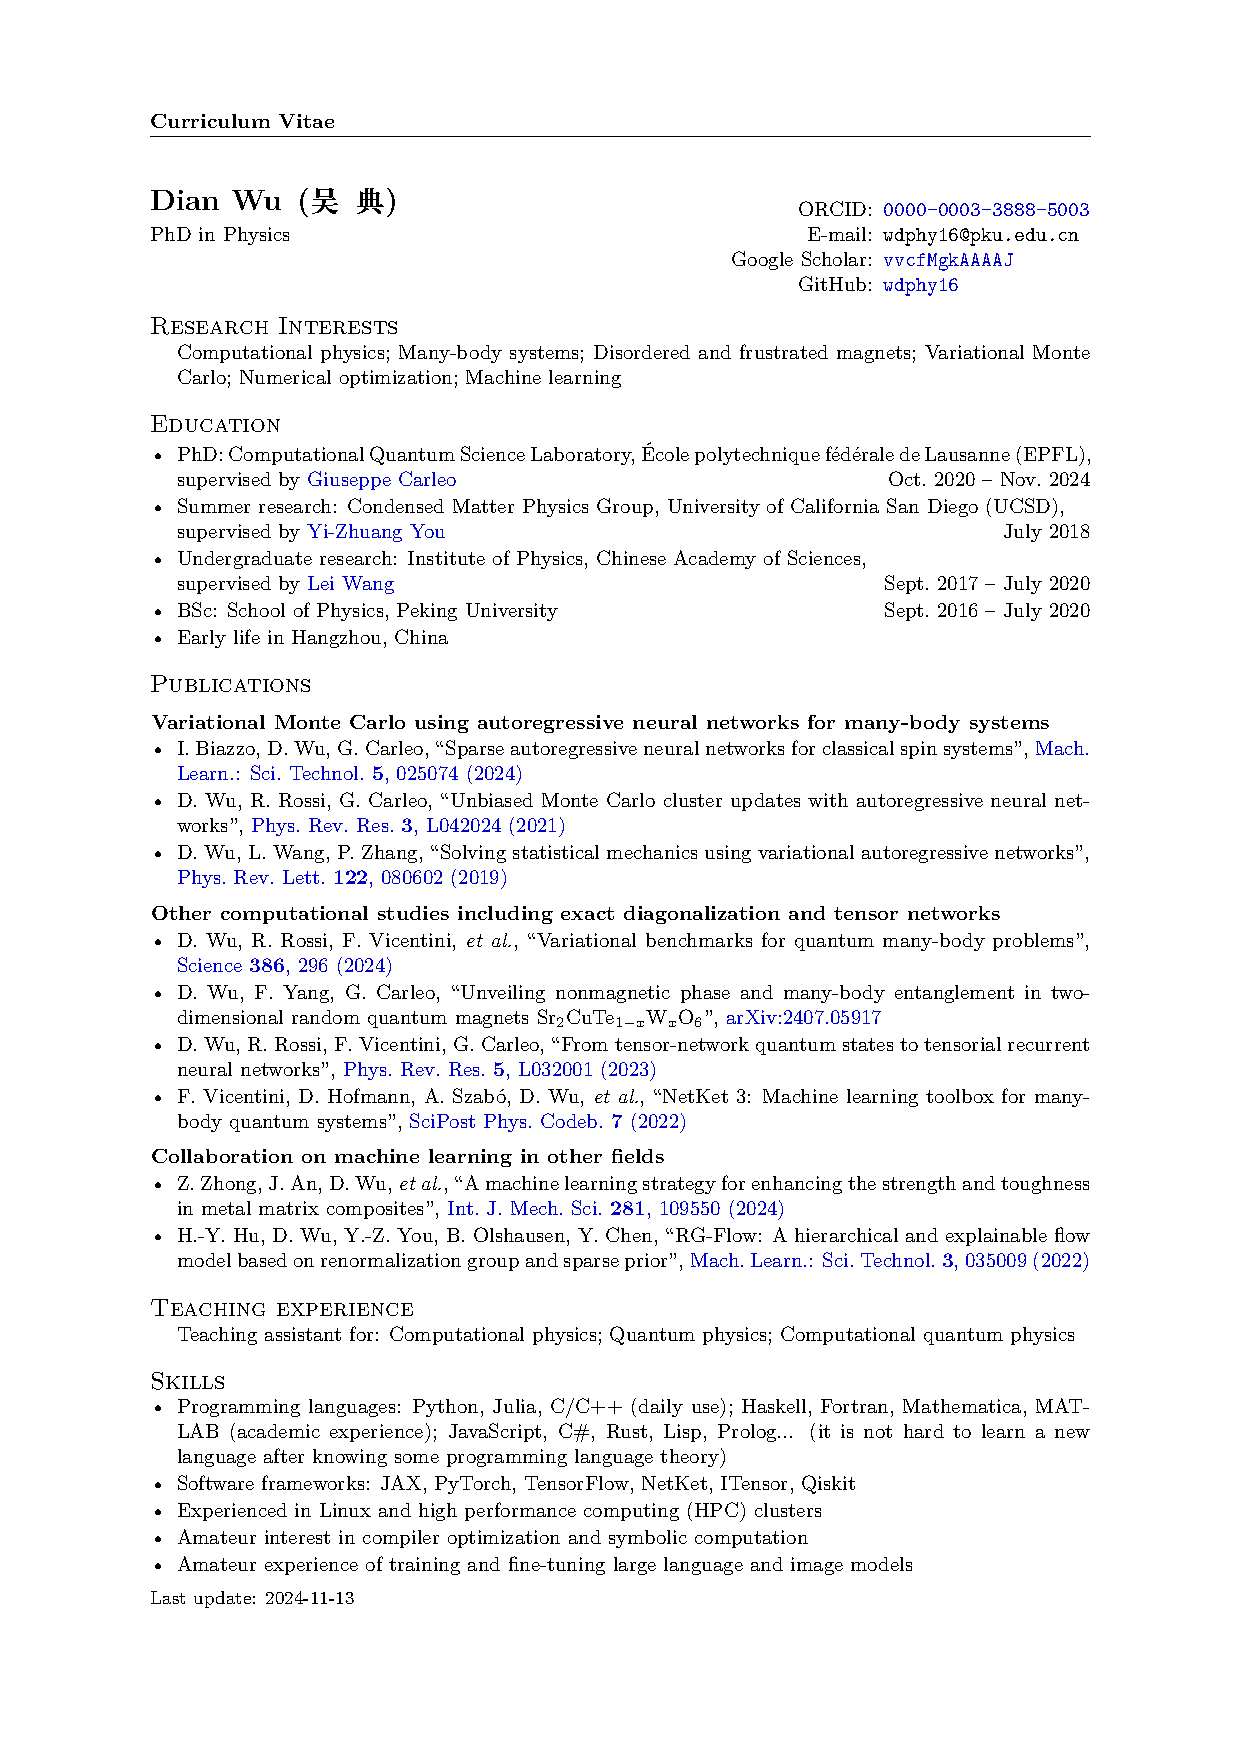
\includepdf{tail/cv_page}
 % TODO
\end{document}
